%%%%%%%%%%%%%%%%%%%%%%%%%%%%%%%%%%%%%%%%%%
%                                        %
% Szablon pracy dyplomowej magisterskiej % 
%                                        %
%%%%%%%%%%%%%%%%%%%%%%%%%%%%%%%%%%%%%%%%%%


\documentclass[a4paper,twoside,12pt]{book}
\usepackage[utf8]{inputenc}                                      
\usepackage[T1]{fontenc}  
\usepackage{amsmath,amsfonts,amssymb,amsthm}
\usepackage[british,polish]{babel} 
\usepackage{indentfirst}
\usepackage{lmodern}
\usepackage{graphicx} 
\usepackage{hyperref}
\usepackage{booktabs}
\usepackage{tikz}
\usepackage{multirow}
\usepackage{pgfplots}
\usepackage{mathtools}
\usepackage{geometry}
\usepackage{colortbl}
\usepackage{adjustbox}
\usepackage[nolists,nomarkers]{endfloat}  % wersja pracy z~rysunkami i~tabelami na końcu
\usepackage{siunitx}
\usepackage[ruled]{algorithm2e}
\usepgfplotslibrary{units}
\usepackage[page]{appendix} % toc,
\renewcommand{\appendixtocname}{Dodatki}
\renewcommand{\appendixpagename}{Dodatki}
\renewcommand{\appendixname}{Dodatek}

\newenvironment{algorytm}[1][]
  {\renewcommand{\algorithmcfname}{Algorytm}% Update algorithm name
   \begin{algorithm}[#1]%
  }{\end{algorithm}}

\usepackage{setspace}
\onehalfspacing


\frenchspacing

\usepackage{listings}
\lstset{
	language={},
	basicstyle=\ttfamily,
	keywordstyle=\lst@ifdisplaystyle\color{blue}\fi,
	commentstyle=\color{gray}
}

%%%%%%%%%

\usepackage{thmtools}                    % theorem customisation
\declaretheorem[style=definition,qed=$\blacktriangle$,numbered=yes,name=Przyk{\l}ad]{example}


%%%% TODO LIST GENERATOR %%%%%%%%%

%\usepackage{tikz}
%\usepackage{manfnt}   % dangerous sign 
\usepackage{color}
\definecolor{brickred}      {cmyk}{0   , 0.89, 0.94, 0.28}

%%%%%%%%%%%%%% END OF TODO LIST GENERATOR %%%%%%%%%%%

%%%%%%%%%%%% ZYWA PAGINA %%%%%%%%%%%%%%%
% brak kapitalizacji zywej paginy
\usepackage{fancyhdr}
\pagestyle{fancy}
\fancyhf{}
\fancyhead[LO]{\nouppercase{\it\rightmark}}
\fancyhead[RE]{\nouppercase{\it\leftmark}}
\fancyhead[LE,RO]{\it\thepage}


\fancypagestyle{tylkoNumeryStron}{%
   \fancyhf{} 
   \fancyhead[LE,RO]{\it\thepage}
}

\fancypagestyle{NumeryStronNazwyRozdzialow}{%
   \fancyhf{} 
   \fancyhead[LO]{\nouppercase{\it\rightmark}}
   \fancyhead[RE]{\nouppercase{\it\leftmark}}
   \fancyhead[LE,RO]{\it\thepage}
}


%%%%%%%%%%%%% OBCE WTRETY  
\newcommand{\obcy}[1]{\emph{#1}}
\renewcommand{\ang}[1]{{\selectlanguage{british}\obcy{#1}}}
%%%%%%%%%%%%%%%%%%%%%%%%%%%%%

% polskie oznaczenia funkcji matematycznych
\renewcommand{\tan}{\operatorname {tg}}
\renewcommand{\log}{\operatorname {lg}}

% jeszcze jakies drobiazgi

\newcounter{stronyPozaNumeracja}

\newcommand{\hcancel}[1]{%
    \tikz[baseline=(tocancel.base)]{
        \node[inner sep=0pt,outer sep=0pt] (tocancel) {#1};
        \draw[red] (tocancel.south west) -- (tocancel.north east);
    }%
}%

\newcommand{\miesiac}{%
  \ifcase\the\month
  \or styczeń% 1
  \or luty% 2
  \or marzec% 3
  \or kwiecień% 4
  \or maj% 5
  \or czerwiec% 6
  \or lipiec% 7
  \or sierpień% 8
  \or wrzesień% 9
  \or październik% 10
  \or listopad% 11
  \or grudzień% 12
  \fi}


%%%%%%%%%%%%%%%%%%%%%%%%%%%%%%%%%%%%%%%%%%%%%%
% Helvetica font macros for the title page:
\newcommand{\headerfont}{\fontfamily{phv}\fontsize{18}{18}\bfseries\scshape\selectfont}
\newcommand{\titlefont}{\fontfamily{phv}\fontsize{18}{18}\selectfont}
\newcommand{\otherfont}{\fontfamily{phv}\fontsize{14}{14}\selectfont}

%%%%%%%%%%%%%%%%%%%%%%%%%%%%%%%%%%%%%%%%%%%%%%
%%%%%%%%%%%%%%%%%%%%%%%%%%%%%%%%%%%%%%%%%%%%%%
%%%%%%%%%%%%%%%%%%%%%%%%%%%%%%%%%%%%%%%%%%%%%%
%%%%%%%%%%%%%%%%%%%%%%%%%%%%%%%%%%%%%%%%%%%%%%
%%%%%%%%%%%%%%%%%%%%%%%%%%%%%%%%%%%%%%%%%%%%%%
%%%%%%%%%%%%%%%%%%%%%%%%%%%%%%%%%%%%%%%%%%%%%%
%%%%%%%%%%%%%%%%%%%%%%%%%%%%%%%%%%%%%%%%%%%%%%


\newcommand{\autor}{Przemysław Gepfert}
\newcommand{\promotor}{dr hab. inż. Krzysztof Simiński}
\newcommand{\konsultant}{dr inż. Imię Nazwisko}
\newcommand{\tytul}{Predykcja zachowań zawodników podczas meczu piłki siatkowej}
\newcommand{\polsl}{Politechnika Śląska}
\newcommand{\wydzial}{Wydział Automatyki, Elektroniki i~Informatyki}


\begin{document}
%\kslistofremarks 

%\pglistofremarks
	
%%%%%%%%%%%%%%%%%%  STRONA TYTULOWA %%%%%%%%%%%%%%%%%%%
\pagestyle{empty}
{
	\newgeometry{top=2.5cm,%
	             bottom=2.5cm,%
	             left=3cm,
	             right=2.5cm}
	\sffamily
	\rule{0cm}{0cm}
	
	\begin{center}
	
\includegraphics[width=0.4\textwidth]{politechnika_sl_logo_bw_poziom_pl.eps}
	\end{center} 
	\vspace{1cm}
	\begin{center}
	\headerfont \polsl
	\end{center}
	\begin{center}
	\headerfont \wydzial
	\end{center}
	\vfill
	\begin{center}
	\titlefont Praca dyplomowa magisterska
	\end{center}
	\vfill
	
	\begin{center}
	\otherfont \tytul\par
	\end{center}
	
	\vfill
	
	\vfill
	 
	\noindent\vbox
	{
		\hbox{\otherfont autor: \autor}
		\vspace{12pt}
		\hbox{\otherfont kierujący pracą: \promotor}
		%\vspace{12pt}
		%\hbox{\otherfont konsultant: \konsultant}
	}
	\vfill 
 
   \begin{center}
   \otherfont Gliwice,  \miesiac\ \the\year
   \end{center}	
	\restoregeometry
}
  

\cleardoublepage
 

\rmfamily
\normalfont

%%%%%%%%%%%%%%%%%%%%% oswiadczenie o~udostępnianiu pracy dyplomowej %%%%%%%%%%%%%%%%%%%
\cleardoublepage

\begin{flushright}
załącznik nr 2 do zarz. nr 97/08/09 
\end{flushright}

\vfill  

\begin{center}
\Large\bfseries Oświadczenie
\end{center}

\vfill

Wyrażam  zgodę / Nie wyrażam zgody*  na  udostępnienie  mojej  pracy  dyplomowej / rozprawy doktorskiej*.

\vfill

Gliwice, dnia \today

\vfill

\rule{0.5\textwidth}{0cm}\dotfill 

\rule{0.5\textwidth}{0cm}
\begin{minipage}{0.45\textwidth}
{\begin{center}(podpis)\end{center}}
\end{minipage} 

\vfill

\rule{0.5\textwidth}{0cm}\dotfill 

\rule{0.5\textwidth}{0cm}
\begin{minipage}{0.45\textwidth}
{\begin{center}\rule{0mm}{5mm}(poświadczenie wiarygodności podpisu przez Dziekanat)\end{center}}
\end{minipage}


\vfill

* podkreślić właściwe

 


%%%%%%%%%%%%%%%%%%%%%% oswiadczenie promotora o~spełnieniu wymagań formalnych %%%%%%%%%%%%%%%%%%%
%\cleardoublepage
%
%\rule{1cm}{0cm}
%
%\vfill  
%
%\begin{center}
%\Large\bfseries Oświadczenie promotora
%\end{center}
%
%\vfill
%
%Oświadczam, że praca „\tytul” spełnia wymagania formalne pracy dyplomowej magisterskiej.
%
%\vfill
%
%
%
%\vfill
%
%Gliwice, dnia \today
%
%\rule{0.5\textwidth}{0cm}\dotfill 
%
%\rule{0.5\textwidth}{0cm}
%\begin{minipage}{0.45\textwidth}
%{\begin{center}(podpis promotora)\end{center}}
%\end{minipage} 
%
%\vfill
%
%%\rule{0.5\textwidth}{0cm}\dotfill 
%%
%%\rule{0.5\textwidth}{0cm}
%%\begin{minipage}{0.45\textwidth}
%%{\begin{center}\rule{0mm}{5mm}(poświadczenie wiarygodności podpisu przez Dziekanat)\end{center}}
%%\end{minipage}
%%
%%
%%\vfill

 

\cleardoublepage


%%%%%%%%%%%%%%%%%% SPIS TRESCI %%%%%%%%%%%%%%%%%%%%%%
\pagenumbering{Roman}
\pagestyle{tylkoNumeryStron}
\tableofcontents

%%%%%%%%%%%%%%%%%%%%%%%%%%%%%%%%%%%%%%%%%%%%%%%%%%%%%
\setcounter{stronyPozaNumeracja}{\value{page}}
\mainmatter
\pagestyle{NumeryStronNazwyRozdzialow}

%%%%%%%%%%%%%% wlasciwa tresc pracy %%%%%%%%%%%%%%%%%

\chapter{Wstęp}

Siatkówka w~XXI wieku stała się dyscypliną, w~której o~zwycięstwie jednej z~dwóch wyrównanych drużyn często decydują najdrobniejsze szczegóły. Przygotowanie motoryczne zawodników oraz ich wyszkolenie techniczne stoi na coraz to wyższym poziomie, przez co każdy z~zespołów coraz to większą rolę przykłada także do analizy taktycznej. Rozrastające się sztaby trenerskie poświęcają wiele godzin i~dni, by jak najlepiej przygotować drużynę od strony taktycznej na nadchodzącego przeciwnika. W~tym celu z~pomocą przychodzą programy komputerowe pozwalające na tworzenie i~analizę statystyk siatkarskich.

Statystyki siatkarskie są to dane opisujące przebieg kolejnych akcji w~meczu. Specjalnie przeszkoleni statystycy siatkarscy zapisują w~programie do statystyk szereg informacji odnośnie każdego odbicia jakie ma miejsce w~trakcie meczu. Zebrane w~ten sposób dane pozwalają na wyszukiwanie różnego rodzaju słabych stron i~zależności powtarzających się w~grze danej drużyny. Analiza opiera się przede wszystkim na generowaniu raportów liczbowych na podstawie danych spełniających wybrane przez statystyka kryteria i~wyszukiwaniu w~nich wyróżniających się wartości, jak na przykład zauważenie, że analizowany zawodnik znajdując się w~konkretnym ustawieniu ponad 60\% piłek wystawia na lewe skrzydło. Nie jest jednak określony kierunek poszukiwań, który pozwoli znaleźć najciekawsze dla trenerów zależności. Dlatego też sztaby trenerskie poświęcają sporą ilość czasu, by znaleźć i~przekazać swoim zawodnikom jak najwięcej informacji na temat najbliższego przeciwnika. W~ostatecznym rozrachunku może okazać się, że zdobyta wiedza pozwoli zdobyć jeden punkt więcej w~secie czy meczu, który przeważy o~zwycięstwie jednej lub drugiej drużyny. 

Zamiast przeszukiwania i~analizowania przez statystyków kolejnych wybranych pozbiorów posiadanych danych tego typu analiza mogłaby zostać przeprowadzona za pomocą technik eksploracji danych, czyli wykorzystania mocy obliczeniowej komputerów do odkrywania wiedzy z~danych. W~ten sposób wielogodzinną pracę sztabów trenerskich zastąpiłyby coraz to szybsze komputery, dając jednocześnie wyniki, które wcale nie musiałyby zostać ostatecznie wykryte przez trenerów, gdyż eksploracja danych pozwala bardzo często znajdować zależności ukryte dla człowieka, właśnie ze względu na ograniczone możliwości czasowe.

W ten sposób powstał pomysł na pracę, której celem jest przetwarzanie i~analiza danych opisujących zagrania poszczególnych zawodników podczas meczów piłki siatkowej. Problem polega na wykorzystaniu metod eksploracji danych z~meczów siatkarskich w~celu znalezienie zależności, trudno zauważalnych dla człowieka, w~grze poszczególnych zawodników, jak i~całej drużyny oraz zbadaniu wpływu wykorzystania zdobytej dzięki temu wiedzy na końcowy wynik meczu. Otrzymane wyniki mają za zadanie pomóc trenerom piłki siatkowej przewidywać najbardziej prawdopodobne zagrania zawodników drużyny przeciwnej oraz wybrać najlepsze możliwe rozwiązania dotyczące zagrań zawodników własnej drużyny, tak by zwiększyć szansę na zdobycie kolejnych punktów w~meczu i~co za tym idzie również zwiększyć szansę na osiągnięcie końcowego sukcesu w~postaci zwycięstwa własnej drużyny w~meczu. Wyniki otrzymanej analizy powinny być wizualizowane w~aplikacji desktopowej, a~także zapisywane w~postaci przedmeczowego raportu, tworzonego do analizy taktycznej gry drużyny przeciwnej.

W rozdziale \ref{roz:analiza-tematu} zawarta została analiza statystyk siatkarskich, wraz z~omówieniem dokładniej pojęcia eksploracji danych i~metod użytych w~badaniach. Rozdział \ref{roz:przedmiot-pracy} przedstawia narzędzia oraz algorytmy wybrane do realizacji projektu. W~rozdziale \ref{roz:badania} przedstawiono przeprowadzone badania naukowe wraz z wyciągniętymi na ich podstawie wnioskami. Rozdział \ref{roz:podsumowanie} jest natomiast podsumowaniem całej pracy, zawierającym także pomysł na dalszy jej rozwój i~wykorzystanie przez kluby.

Cała praca, w~tym przeprowadzone badania, zostały zrealizowane samodzielnie, konsultując kolejne etapy działań i~otrzymywane wyniki z~promotorem pracy oraz profesjonalnym statystykiem siatkarskim, otrzymując dzięki temu wskazówki również pod kątem samego wykorzystania opisywanej pracy w~praktyce. Separatorem liczb dziesiętnych w~całej pracy jest przecinek.


\chapter{Statystyki siatkarskie}
\label{roz:analiza-tematu}

\section{Siatkówka}
\label{roz:siatkowka}

Siatkówka jest grą zespołową, w~której na boisku po dwóch stronach siatki rywalizują drużyny złożone z~sześciu zawodników. Celem obu drużyn jest zdobywanie punktów za wygrane akcje, w~których piłka przebijana jest nad siatką. Akcja rozpoczyna się od zagrywki zza boiska wykonywanej przez zawodnika jednej z~drużyn. Piłka następnie jest przyjmowana przez drużynę przeciwną, która wliczając przyjęcie ma trzy odbicia by przebić piłkę na drugą stronę siatki. Jeden zawodnik nie może jednak odbić piłki dwa razy z~rzędu. Oprócz zagrywki oraz przyjęcia w~trakcie akcji wyróżnia się także takie zagrania jak: rozegranie piłki, atak, blok oraz obrona. Po udanym przyjęciu piłka zostaje rozegrana do jednego z~zawodników wykonujących atak. Drużyna przeciwna stara się zablokować lub obronić atak rywali po czym sama ma możliwość rozegrania i~zaatakowania piłki. Akcja kończy się gdy piłka dotknie boiska po którejś ze stron, lub któryś z~zawodników wykona błędne zagranie, jak na przykład dotknięcie siatki. Punkt jest zdobyty przez drużynę, gdy piłka spadnie na boisko drużyny przeciwnej lub przeciwnik przebije piłkę w~aut, czy też wykona błędne zagranie. Gra toczy się zwykle do trzech wygranych setów rozgrywanych do 25 punktów (poza piątym setem rozgrywanym do 15 punktów). 

Każdą ze stron boiska do siatkówki dzieli się na 6 stref ukazanych na rysunku \ref{fig:strefy}. Strefy 2, 3 oraz 4 znajdują się pod siatką, czyli w~pierwszej linii boiska, natomiast strefy 1, 5 oraz 6 znajdują się w~drugiej linii. Zawodnik będący w~drugiej linii może wykonywać atak tylko zza wyznaczonej na boisku linii trzeciego metra. Przed rozpoczęciem każdego seta trener zespołu ustala wyjściowy skład drużyny, wypisując numery zawodników rozpoczynających seta w~określonej strefie. Po zdobyciu punktu przez drużynę przyjmującą piłkę następuje rotacja zawodników tej drużyny zgodnie z~ruchem wskazówek zegara. W~przypadku zawodników zawodowo uprawiających tą dyscyplinę sportu występuje specjalizacja gry na poszczególnych pozycjach. Wyróżnia się pięć różnych pozycji:
\begin{itemize}
\item rozgrywający,
\item przyjmujący,
\item atakujący,
\item środkowy,
\item libero.
\end{itemize}
Wybór pozycji dla poszczególnych zawodników dokonywany jest przez trenerów zazwyczaj już w~okresie młodzieżowym i~wynika głównie z~warunków fizycznych zawodników (przede wszystkim wzrostu oraz wyskoku), a~także techniki odbić piłki. Każda z~wymienionych pozycji charakteryzują się bowiem innymi zadaniami na boisku, a~mianowicie:
\begin{itemize}
\item rozgrywający odpowiedzialny jest za rozegranie (wystawę) piłki przyjmowanej po zagrywce, a~także obronionej po ataku zawodnika drużyny przeciwnej;
\item przyjmujący odpowiada za przyjmowanie zagrywek oraz wykonanie późniejszego ataku (w większości ustawień z~tak zwanego lewego skrzydła);
\item atakujący ma za zadanie przede wszystkim zdobyć jak najwięcej punktów atakiem (wykonywanym z~prawego skrzydła);
\item środkowy jest odpowiedzialny głównie za blokowanie ataków drużyny przeciwnej, jednak sam również wykonuje atak z~piłek rozegranych na środek siatki;
\item libero, podobnie jak przyjmujący, odpowiada za przyjmowanie zagrywek, jednak nie może wykonywać ataków - zamiast atakowania do głównych zadań zawodnika na pozycji libero należy także obrona piłek atakowanych przez drużynę przeciwną.
\end{itemize}

\begin{figure}[t]
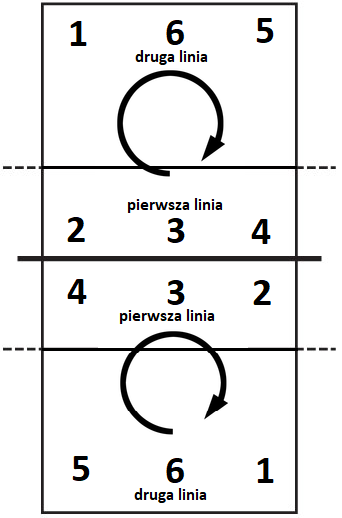
\includegraphics[width=6cm]{strefy}
\centering
\caption{Numery poszczególnych stref na boisku wraz z~kierunkiem rotacji.}
\label{fig:strefy}
\end{figure}

W wyjściowym składzie drużyny znajduje się jeden rozgrywający, dwóch przyjmujących, dwóch środkowych oraz atakujący. Zawodnik libero zmienia się z~zawodnikami grającymi na pozycji środkowego w~momencie gdy po rotacji drużyny znajdą się oni w~drugiej linii. Od numeru strefy w~jakiej znajduje się rozgrywający nazywane jest ustawienie całej drużyny. Przykładowo gdy rozgrywający znajduje się w~strefie czwartej drużyna jest w~czwartym ustawieniu, określanym również jako P4 (od ang. \ang{position 4}). W~każdym z~ustawień drużyna przyjmująca inaczej ustawiona jest do przyjęcia zagrywki (rys.~\ref{fig:ustawienia}). 
\begin{figure}[t]
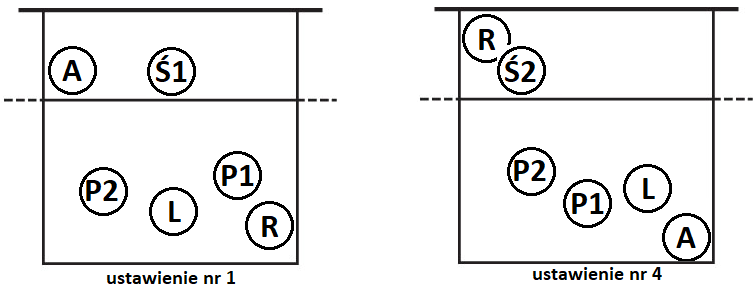
\includegraphics[width=\textwidth]{ustawienia}
\centering
\caption{Przykładowe ustawienia nr 1 oraz nr 4 do przyjęcia zagrywki (R -- rozgrywający, A~-- atakujący, P1 -- pierwszy przyjmujący, P2 -- drugi przyjmujący, Ś1 -- pierwszy środkowy, Ś2 -- drugi środkowy, L -- libero.}
\label{fig:ustawienia}
\end{figure} 

Zawodnicy wykonujący ataki cechują się zwykle wysokim wzrostem i~dużą siłą, która pomaga w~zdobywaniu punktów. Siatkówka jest jednak przede wszystkim dyscypliną techniczną. Szczególnie przyjęcie oraz rozegranie piłki wymaga dużych umiejętności technicznych, by odbita piłka za każdym razem zmierzała w~pożądanym kierunku. Również podczas ataku ze skrzydeł zawodnicy niejednokrotnie zamiast na mocny atak decydują się na rozwiązania techniczne, takie jak obicie bloku czy kiwnięcie piłki, które wykonane w~odpowiednim, zaskakującym dla zawodników drużyny przeciwnej momencie pozwala na równie skuteczne zdobycie punktów. Zaskakiwanie rywali to także główne zadanie rozgrywającego, który rozgrywając piłki do swoich zawodników musi poza dokładnością wystaw starać się zgubić blok drużyny przeciwnej. Czym mniej przewidywalna jest gra rozgrywającego tym cięższe zadanie mają blokujący by zatrzymać ataki rywali. Obie drużyny starają się więc oprócz wykonywania jak najdokładniej pojedynczych zagrań również zaskakiwać wyborami swoich rywali. By móc analizować zarówno jakość odbić poszczególnych zawodników jak i~dokonywane przez nich wybory wymyślono sposób zapisywania przebiegu meczu w~postaci statystyk siatkarskich.

\section{Statystyki siatkarskie}
\label{roz:statystyki-siatkarskie}

Analiza statystyczna obecnie nieodzownie towarzyszy prawie wszystkim profesjonalnym drużynom siatkarskim. Na podstawie statystyk, możliwych do tworzenia zarówno w~trakcie rozgrywanego meczu jak i~po meczu na podstawie nagrań wideo, trenerzy mogą przeanalizować pod wieloma względami grę zarówno własnej drużyny jak i~przeciwnika \cite{bib:volleyballStats}. Analiza gry własnej drużyny wykonywana jest przede wszystkim pod kątem wyszukania które elementy gry wymagają poprawy na treningach, a~także w~celu wyboru optymalnego składu czy też dokonania zmiany w~trakcie meczu. W~trakcie sezonu statystyki wykorzystywane są jednak w~szczególności aby przeanalizować grę najbliższego przeciwnika i~przygotować taktykę na najbliższy mecz. W~tym celu wyszukiwane są słabe
strony w~grze drużyny przeciwnej oraz zależności powtarzające się wielokrotnie w~grze zarówno całej drużyny jak i~jej poszczególnych zawodników.

Analizując grę najbliższego przeciwnika sztaby trenerskie najczęściej najwięcej czasu poświęcają analizie gry rozgrywających. Przewidywanie gry rozgrywających pozwala, jak wcześniej wspomniano, na dużo skuteczniejsze ustawienie bloku, co ma znaczący wpływ na utrudnieniu przeciwnikowi zdobycia punktu atakiem. Odbija się to więc często na skutecznej grze drużyny przewidującej w~elemencie bloku oraz obrony, ale przede wszystkim ma wpływ na wybory atakujących po stronie rozpracowywanego rozgrywającego. Zwykle bowiem zawodnicy atakujący są zmuszeni wybrać całkiem inną formę ataku przy szczelnie ustawionym potrójnym bloku niż przy bloku pojedynczym. Podobnie jednak sytuacja wygląda, jeśli chodzi o~wybory rozgrywających w~zależności od jakości przyjęcia. Dużo trudniej przewidzieć wystawę rozgrywającego przy przyjęciu perfekcyjnym, niż przy piłce pozwalającej rozgrywającemu tylko wystawić piłkę nad siebie. Kolejne zagrania są więc bardzo mocno od siebie zależne, a~to jakie elementy mają największy wpływ na wybory zawodników na poszczególnych pozycjach, jest właśnie podstawą analizy opisywanych w~tej pracy badań.

Ze względu na dużą szybkość gry dokładne zapisywanie przebiegu poszczególnych akcji nie należy do łatwych zadań. W~szczególności w~przypadku dłuższych wymian z~wieloma obronami. Z~tego powodu powstały specjalistyczne programy do tworzenia statystyk. Przez długi czas na rynku programów do statystyk występował monopol firmy Data Project \cite{bib:inzynier}. W~ostatnich latach na popularności zyskuje program polskiej firmy Volleystation. Oba programy są bardzo zbliżone do siebie. Oprócz samego tworzenia statystyk programy te pozwalają na przeglądanie szeregu raportów i~wykresów ułatwiających wyszukiwania różnego rodzaju zależności. Nie zawsze jednak wiadomo w~jakim kierunku przeszukiwać posiadane dane, by znaleźć interesujące dla sztabu trenerskiego informacje. Nauka obsługi samego programu wymaga specjalistycznych szkoleń, które przechodzą przyszli statystycy. Jednym z~głównych elementów takich szkoleń jest nauka sposobu zapisywania kodu akcji.

\subsection{Kodowanie przebiegu akcji}
\label{roz:analiza-kodu}

Zapisy z~meczów tworzone przez statystyków siatkarskich przechowywane są w~plikach
o rozszerzeniu \texttt{dvw} (ang. \ang{Data Volley}). Pojedynczy plik o~tym rozszerzeniu zawiera zapis całego jednego meczu. Na zapis ten składją się następujące informacje:
\begin{itemize}
\item data, sezon i~kategoria rozegranego meczu,
\item zespoły uczestniczące w~meczu,
\item wyniki poszczególnych setów,
\item lista zawodników obu zespołów,
\item zapisy każdej z~rozegranych w~meczu akcji.
\end{itemize}

Ostatni podpunkt stanowi źródło danych wykorzystywanych do analizy w~opisywanej pracy. Zapisy te posiadają informacje o~każdym zarejestrowanym przez statystyka siatkarskiego odbiciu piłki w~meczu. W~celu ujednolicenia zapisów kodu przez statystyków wymyślona została odpowiednia składnia. Zapis informacji o~pojedynczym odbiciu składa się z~20 znaków o~określonych dozwolonych wartościach na każdej z~pozycji. Pozycje poszczególnych znaków odpowiadają odpowiednim informacjom, opisanym w~tabeli \ref{tab:skladnia}.

\begin{table}
\centering
\caption{Informacje odpowiadające poszczególnym pozycjom w~składni zapisów akcji.}
\label{tab:skladnia}
\begin{tabular}{rl}
	\toprule
	pozycja     & informacja \\
	\midrule
	1       &  zespół zawodnika wykonującego zagranie (gospodarz ,,*'', gość ,,a''),  \\
	2-3 &  numer zawodnika (00-99) \\
	4   &  rodzaj zagrania \\
	5  &  typ zagrania \\
	6     &  jakość wykonania zagrania \\
	7-8       &  kombinacja ataku/ruch rozgrywającego \\
	9   &   kierunek zagrania \\
	10   &   strefa początkowa \\
	11  &   strefa końcowa \\
	12  &   dokładna strefa końcowa \\
	13  &   typ umiejętności \\
	14  &   liczba zawodników (głównie wykorzystywana do opisu bloku) \\
	15  &   dodatkowa informacja \\
	16-20  &   miejsce na kod własny statystyka \\
	\bottomrule
\end{tabular}
\end{table}

Dla każdego z~rodzajów zagrań (zagrywka, przyjęcie, atak, blok, obrona, rozegrania, dogranie) inne znaczenie mają znaki dla takich pozycji jak typ zagrania, jakość wykonania zagrania czy typ umiejętności. Przykładowo dla zagrywki oznaczanej poprzez ,,S'' (od ang. \ang{Serve}) typ zagrania ,,H'' (od ang. \ang{High}) oznacza zagrywkę typu float, natomiast dla ataku oznaczanego poprzez ,,A'' (od ang. \ang{Attack}) typ zagrania ,,H'' oznacza atak z~piłki wysokiej. To jakie znaki są dozwolone i~co określają na poszczególnych pozycjach jest elementem szkoleń jakie przechodzą osoby, które chcą zostać statystykami siatkarskimi.
 
Z tych 20 znaków umożliwiających opis danego zagrania tylko pierwsze 6 jest obowiązkowe do wypełnienia przez statystyka. Kolejne 6 znaków zwykle jest także wypełnianych, gdyż zapisane są na nich m.in. informacje o~kierunkach zagrań, które później są dokładnie analizowane. Znaki na pozycjach od 13 do 15 są wypełniane już dużo rzadziej, natomiast tylko niektórzy statystycy używają ostatnich 5~znaków do własnego sposobu zapisu dodatkowych informacji. Ilość zapisywanych przez statystyków informacji związana jest również z~ich biegłością w~obsłudze programu do statystyk. Początkujący statystycy mają czasem problem zanotować nawet podstawowe informacje odnośnie kolejnych odbić w~akcji, szczególnie w~dłuższych akcjach składających się z~kilkunastu odbić. Znaki na pozycjach nieuzupełnionych przez statystyka w~końcowym zapisie przedstawione są w~postaci znaku tyldy (,,\textasciitilde'').

Każdy wiersz zapisu akcji oprócz 20 znaków dotyczących odbicia posiada również dodatkowe informacje dodane przez program do statystyk. Są to m.in. informacje o~wyniku oraz czasie meczu i~numerach zawodników znajdujących się na poszczególnych pozycjach w~ustawieniu zespołu. Przy pięciosetowych meczach liczba wierszy, z~których składa się zapis meczu dochodzi do dwóch tysięcy.

\section{Eksploracja danych}
\label{roz:eksploracja-danych}
W celu uzyskania wiedzy na podstawie zgromadzonych w~bazie danych informacji używane są różne techniki eksploracji danych. Wykorzystywana jest w~nich moc obliczeniowa komputerów, która pozwala wyszukać zależności często ukryte dla człowieka. Wynika to ze względu na ograniczenia czasowe dotyczące przeszukiwania posiadanych danych. Tych natomiast zbieranych jest coraz więcej przez różnego rodzaju czujniki stosowane w~urządzeniach elektronicznych czy też systemy informatyczne wykorzystywane w~firmach do rejestrowania transakcji lub przechowywania informacji o~klientach. To nagromadzanie danych spowodowało rozwój technologii eksploracji danych pozwalającej wykorzystywać zdobytą w~ten sposób wiedzę na przykład do usprawnienia tworzonych systemów i~uzyskiwania w~ten sposób większych przychodów.

Występuje wiele metod eksploracji danych \cite{bib:przegladKlasyfikacji}. Jako najpopularniejsze z~nich wyróżnia się:
\begin{itemize}
\item grupowanie,
\item odkrywanie asocjacji,
\item odkrywanie klasyfikacji,
\item wykrywanie zmian i~odchyleń,
\item analizowanie przebiegów czasowych,.
\end{itemize}

W opisywanej pracy podjęto próbę wykorzystania pierwszych trzech wymienionych metod, w~związku z~czym to one zostały poniżej dokładniej opisane.

\subsection{Grupowanie}
Grupowanie (ang. \ang{data clustering}) \cite{bib:clustering} to metoda wyszukiwania w~ danych skończonych zbiorów klas obiektów, czyli grup nazywanych klastrami, do których należą obiekty posiadające zbliżone cechy lub, w~przypadku możliwości zastosowania podejścia geometrycznego, będące biskie względem zadanej odległości. Prostym przykładem może być dzielenie ubrań według kolorów przed ich wypraniem. Podzielić je można na różną liczbę klastrów odpowiadającym każdemu kolorowi jaki występuje wśród ubrań, lub na przykład jedynie na dwa klastry: ubrania białe oraz kolorowe. Problemem może być już jednak przydzielenie do odpowiedniego klastra białej koszulki z~wielokolorowymi wzorami. Grupowanie często jest zabiegiem bardzo dynamicznym, gdyż w~zależności od tego jakie rekordy zostaną dodane do bazy danych podział na klastry może się całkowicie zmienić. Przykładem może być ponownie podzielenie ubrań na dwa klastry, jednak tym razem według ich różnych cech. Mając w~zbiorze 4 ubrania: białe skarpetki, białą koszulkę, czarne spodnie oraz czarną kurtkę najłatwiej podzielić zbiór ponownie na klastry odpowiadające białemu oraz czarnemu kolorowi, jednak gdy do zbioru dodamy kolejne 4 koszulki w~różnych kolorach podział na klastry może być następujący: koszulki oraz ubrania które nie są koszulkami. W~przypadku danych biznesowych zbieranych przez firmy dynamiczne zmiany mogą dotyczyć charakterystyki klientów korzystających z~usług tej firmy, która zmienia się w~zależności od panującej na rynku sytuacji oraz oferowanych w~danym czasie usług. Otrzymywany wynik działania jest więc przede wszystkim mocno zależny od oczekiwanej postaci jaką chce się otrzymać.

Algorytmy wykorzystywane do grupowania można podzielić na hierarchiczne oraz niehierarchiczne. W~przypadku tej pierwszej grupy dla badanego zbioru tworzona jest hierarchia klastrów -- klaster najwyższego poziomu zawiera w~sobie wszystkie rekordy, natomiast klastry najniższych poziomów grupują jedynie indentyczne rekordy. Po dokonaniu tego typu podziału użytkownik analizując otrzymane wyniki może dowolnie dobrać liczbę klastrów poruszając się w~górę lub dół otrzymanej hierarchii zwizualizowanej zwykle w~postaci dendrogramu. W~przypadku algorytmów niehierarchicznych użytkownik podaje docelową liczbą klastrów, lub minimalną odległość pozwalającą zakwalifikować rekordy do tego samego klastra. Algorytmy takie iteracyjnie dążą do uzyskania jak najlepszego podziału, czyli takiego w~którym rekordy zaliczone do jednej klasy są najbardziej zbliżone do siebie i~jednocześnie  różnią się znacząco od rekordów należących do innych klas.

Na podstawie otrzymanego dzięki grupowania podziału na klastry przeglądanie zawartości bazy danych może okazać się zdecydowanie łatwiejsze, ale przede wszystkim łatwiej jest wychwycić wśród wyodrębnionych grup pewne prawidłowości, pozwalające na wyciągnięcie różnych wniosków. Łatwiej jest również wyizolować na przykład występujące w~zbiorze błędne dane, odstające wyraźnie od reszty.

\subsection{Odkrywanie asocjacji}
Pojęcie odkrywania reguł asocjacyjnych (ang. \ang{association rules}) zostało wprowadzone w~1993 roku przez R. Agrawala, T. Imielinskiego, A. Swami \cite{bib:associationrules}. Odkrywanie asocjacji polega na wyszukiwaniu różnego rodzaju współzależności występujących w~bazie danych. Zależności te są prezentowane właśnie jako reguły asocjacyjne o~postaci ,,jeśli poprzednik, to następnik'', czyli implikacji \(A \implies B\) (A -- poprzednik, B -- następnik). Poprzednikiem jest zbiór występujących warunków, natomiast następnikiem wniosek wyciągany zwykle gdy te warunki zachodzą. Dodatkowo dla każdej reguły otrzymywane są również dodatkowe wartości określające wspracie i~ufność takiej reguły. Wsparcie (ang. \ang{support}) $s$ dla danej reguły asocjacyjnej \(A \implies B\) jest odsetkiem instancji w~bazie danych, zawierającym $A$ i~$B$, czyli:
\begin{equation}
s = P(A \cap B)
\end{equation}

Ufność (ang. \ang{confidence}) $c$  dla danej reguły asocjacyjnej \(A \implies B\) jest procentem instancji w~bazie danych spełniających $A$, które spełniają również $B$:
\begin{equation}
c = P(B \mid A) = \frac{P(A \cap B)}{P(A)}
\end{equation}
Regułę uznaje się za mocną gdy zarówno jej wsparcie, jak i~ufność są większe lub równe określonym wartościom minimalnym.

Metoda odkrywania reguł asocjacyjnych nazywana jest również analizą koszykową, gdyż bardzo często wykorzystywana jest do badania preferencji zakupowych klientów. Wyszukiwane są wówczas zależności produktów, które poszczególni klienci często kupują razem. Przykładem może być reguła typu ,,jeśli klient kupuje jajka oraz proszek do pieczenia, to zwykle kupi również mąkę''. Na podstawie otrzymanych tego typu reguł można na przykład dokonać odpowiednich zmian w~układzie produktów występujących w~sklepie, tak by klient miał je wszystkie pod ręką, lub aby właśnie przeszedł cały sklep, by je znaleźć, ale przy okazji dokonać zakupu innych produktów, które nie były celem jego pójścia do sklepu.

\subsection{Klasyfikacja}
\label{roz:klasyfikacja}
Klasyfikacja jest metodą polegającą na określeniu, do której ze zdefiniowanych klas należy nowa instancja dodana do zbioru \cite{bib:classification}. Podział zbioru na odpowiednie klasy odbywa się w~tym przypadku na podstawie dostarczonych wcześniej danych treningowych, na podstawie których następuje rozpoznawanie wzorców \cite{bib:pattern}. 

By klasyfikacja następowała odpowiednio szybko, na podstawie danych treningowych tworzone są modele. Jednym z~takich modeli są użyte w~tej pracy drzewa decycyzyjne \cite{bib:decisionTree}. Są to grafy składające się z~węzłów reprezentujących podejmowane decyzje, na przykład na podstawie kolejnych atrybutów oraz krawędzie wychodzące od węzłów, odpowiadające możliwym wariantom decyzji, czyli przykładowo wartościom atrybutu. Na podstawie takiego modelu klasyfikacja danej instancji polega na przejściu od korzenia do liścia i~przypisaniu klasy odpowiadającej otrzymanemu liściowi. W~ten sposób wyznaczenie odpowiedniej klasy wymaga w~najgorszym przypadku porównania jednokrotnie wartości wszystkich atrybutów, jednak algorytmy budowy drzew decyzyjnych, poprzez odpowiedni wybór kolejnych węzłów starają się budować drzewa, które zwykle pozwalają na szybkie klasyfikowanie instancji.

Częstym przykładem jest klasyfikacja pacjentów w~przychodni. Na podstawie szeregu objawów jakie u nich występują można zakwalifikować ich do danej choroby, która najprawdopodobniej u nich występuje. Do budowy klasyfikatora użyty jest zbiór pacjentów, którzy mieli szereg różnych objawów i~przeszli określone choroby. Zbiór danych o~tych pacjentach zostaje podzielony na dane treningowe oraz testowe. Na podstawie wyszukanych zależności od poszczególnych objawów występujących u pacjentów w~zbiorze treningowym budowany jest klasyfikator, który jest następnie weryfikowany na podstawie zbioru testowego. 

Opisany przykład dotyczy, podobnie jak w~przypadku przeprowadzonych w~opisywanej pracy badań, klasyfikacji wieloklasowej, czyli problemu klasyfikacji obserwacji do jednej z~kilku występujących. Problem ten jest nieco bardziej złożony, jednak zwykle zostaje redukowany do skończonej liczby problemów klasyfikacji dwuklasowej (binarnej). Redukcja przeprowadzana jest zazwyczaj za pomocą jednej z~dwoch metod zwanych $one-vs.-rest$ oraz $one-vs.-one$ \cite{bib:oneversus}. Pierwsza z~nich polega na utworzeniu klasyfikatora binarnego dla każdej klasy, traktując przykłady do niej należące
jako przykłady pozytywne, a~wszystkie pozostałe jako negatywne. Druga metoda polega na utworzeniu $\frac{N(N-1)}{2}$ klasyfikatorów binarnych porównujących wszystkie klasy parami. W~pracy wykorzystana została pierwsza z~metod.

Ocena klasyfikatora opiera się przede wszystkim na dokładności klasyfikacji (ang. \ang{accuracy}), czyli procencie badanych instancji, które zostały poprawnie sklasyfikowane. W~przypadku klasyfikacji wieloklasowej dokładność klasyfikacji wyrażana jest wzorem:
\begin{equation}
\text{ACC} = \frac{1}{N} \sum_{k=1}^{|G|} \sum_{x: g(x) = k} I \left(g(x) = \hat{g}(x)\right)
\end{equation}
gdzie:
\begin{align*}
	N &- \text{liczba obserwacji}\\
    G &- \text{zbiór klas}\\
    x &- \text{pojedyncza obserwacja}\\
    g(x) &- \text{funkcja zwracająca wartość atrybutu decyzyjnego dla obserwacji}\\
    \hat{g}(x) &- \text{funkcja klasyfikująca daną obserwację}\\
    I &- \text{funkcja jednostkowa zwracająca 1 dla obserwacji poprawnie sklasyfikowanych}
\end{align*} 

W zależności od potrzeby późniejszego wykorzystywania modelu wyliczane mogą być również inne miary porównujące wyniki \cite{bib:evaluation}. Oceniany może być także czas uczenia i~klasyfikacji lub złożoność struktury, np. rozmiar otrzymanego drzewa decyzyjnego.

\subsection{Selekcja atrybutów}

Duża liczba atrybutów opisujących dany obiekt nie zawsze musi dawać więcej informacji na jego temat. Szczególnie gdy część z~nich jest tylko szumem informacyjnym \cite{bib:szum}. W~przypadku problemu dotyczącego klasyfikacji obiektów większa ilość informacji pozwala nieraz na lepsze dopasowanie danych uczących, tworzących model klasyfikatora, co jednak może odbić się na zdecydowanie gorszej klasyfikacji nowych obserwacji. Zjawisko to nazywane jest nadmiernym dopasowaniem (ang. \ang{overfitting}). Bardzo często sytuacja ta występuje właśnie ze względu na wielowymiarowość klasyfikowanych obiektów. By temu zapobiec wykorzystywana jest metoda selekcji atrybutów \cite{bib:feature}.

Selekcja atrybutów polega na wyeliminowaniu z~opisu zbioru danych cech nadmiarowych i~nieistotnych. W~tym celu tworzony jest zwykle ranking atrybutów, pozwalający na wykorzystanie do budowy modelu jedynie najbardziej istotnych atrybutów. Istnieją różne metody selekcji atrybutów \cite{bib:metody-selekcji}, które dzielone są zwykle na trzy kategorie:
\begin{itemize}
\item metody filtrujące,
\item metody opakowujące,
\item metody wbudowane.
\end{itemize}

Metody filtrujące dokonują selekcji atrybutów na podstawie konkretnej miary, najczęściej pojedynczego równania. Metody te są szybkie i~niezależne od wybranego następnie modelu analizy danych, przez co często używane są jako krok przygotowania danych.

Metody opakowujące sprawdzają działanie wybranej metody analizy danych na różnych podzbiorach atrybutów. Wyszukiwany w~nich zostaje podzbiór atrybutów maksymalizujący zdefiniowaną skuteczność działania wybranej metody. Zwykle są to metody bardzo złożone obliczeniowo i~najwolniejsze. 

Metody wbudowane wykonują selekcję atrybutów podczas procesu uczenia. Informacja o~ważności atrybutów może zostać następnie pobrana bezpośrednio z~nauczonego klasyfikatora. Szybkość metod wbudowanych zależy od szybkości nauki klasyfikatora.

W przeprowadzonych w~pracy badaniach selekcję atrybutów wykorzystano w~ramach przygotowania danych, użytych następnie do budowy klasyfikatorów. W~związku z~tym wybrana została metoda filtrująca, wykorzystująca do stworzenia rankingu atrybutów przyrost informacji (wzór \ref{wz:przyrostinf}) w~odniesieniu do poszczególnych klas, podobnie jak w~przypadku wyboru węzłów u drzew decyzyjnych. W~ramach budowy drzew decyzyjnych wykorzystywana jest więc dodatkowo wbudowana selekcja atrybutów. 

Wykorzystanie selekcji atrybutów pozwala ograniczyć rozmiary uzyskiwanych rozwiązań. Dzięki temu rozwiązania są więc prostsze do przeanalizowania, a~także pozbawione atrybutów, które mogły tylko zniekształcać posiadane dane. Samo sprawdzenie, które z~atrybutów mają największe znaczenie dla analizowanych danych, może natomiast okazać się już cenną dla badacza informacją, w~związku z~czym jeden z~opisanych w~pracy eksperymentów dotyczy właśnie sprawdzenie rankingu atrybutów dla każdego z~badanych rodzajów zagrań.   

\subsection{Modele eksploracji danych}
Eksploracja danych polega nie tylko na samym wyborze i~zastosowaniu odpowiednich narzędzi. Jest to cały proces wymagający sekwencyjnego przejścia przez kilka etapów. Ze wględu na liczne zastosowania  eksploracji danych powstało wiele propozycji modeli eksploracyjnych \cite{bib:analizaModeliEksploracji}. 

Jednym z~takich modeli jest CRISP-DM (ang. \ang{Cross-Industry Standard Process for Data Mining}) \cite{bib:crispdm} składający się z~sześciu etapów, którymi są:
\begin{itemize}
\item zrozumienie uwarunkowań biznesowych,
\item zrozumienie danych,
\item przygotowanie danych,
\item modelowanie,
\item ewaluacja,
\item wdrożenie.
\end{itemize}

Tego typu model został użyty w~opisywanej pracy. Na wstępie sformułowany został cel i~wymagania projektu. Następnie zebrane zostały dane, które wymagały oceny przydatności, w~szczególności wyboru atrybutów i~klas decyzyjnych. Po przygotowaniu danych nastąpił wybór technik użytych do tworzenia modeli eksploracji danych, które zostały przetestowane oraz ocenione dla różnych wartości parametrów i~wybieranych podzbiorów danych dotyczących badanych typów zagrań, analizując wybranych zawodników. Na koniec rozpoczęte zostały również prace by wykorzystać stworzone modele w~praktyce.

\chapter{Metody analizy statystyk siatkarskich}
\label{roz:przedmiot-pracy}

\section{Narzędzia}
\label{roz:narzedzia}

Program stworzony do predykcji zachowań zawodników podczas meczu piłki siatkowej został zrealizowany w~postaci aplikacji desktopowej, napisanej w~języku programowania Java, z~wykorzystaniem biblioteki JavaFX, umożliwiającej proste stworzenie widoku aplikacji. Głównym powodem wyboru Javy jako język programowania był szereg bibliotek możliwych do użycia zarówno do eksploracji danych jak i~zarządzania bazą danych. Ostatecznie wykorzystane zostały biblioteki Weka oraz SQLite.

Weka (ang. \ang{Waikato Environment for Knowledge Analysis}) to biblioteka otwartego oprogramowania, zawierająca szereg zaimplementowanych algorytmów do analizy danych i~modelowania predykcyjnego. Stworzona została w~latach 90. XX wieku przez Uniwersytet Wakaito w~Nowej Zelandii, jednak wciąż jest powszechnie wykorzystywana w~wielu badaniach i~aktualizowana o~nowo powstałe algorytmy. Biblioteka ta pozwala przeprowadzić zarówno podstawowe jak i~bardziej zaawansowane operacje eksploracji danych, takie jak: wstępne przetwarzanie danych, grupowanie, klasyfikację, asocjację, a~nawet wizualizację danych i~otrzymywanych wyników. Od wersji trzeciej pakiet Weka został napisany w~pełni w~języku Java, w~związku z~czym samo użycie i~wywołanie poszczególnych algorytmów w~programie napisanym również w~Javie jest niezwykle proste. Oprócz tego Weka poprzez interfejs JDBC (ang. \ang{Java Database Connectivity}) umożliwia łatwy dostęp do połączenia z~bazą danych SQL, dzięki czemu wszelkie dane wykorzystywane do eksploracji mogą być wynikami realizowanych zapytań.

SQLite to biblioteka implementująca system zarządzania relacyjną bazą danych SQL (ang. \ang{Structured Query Language}), dzięki czemu daje ona możliwość używania bazy danych bez konieczności dodatkowej konfiguracji \cite{bib:sqlite, bib:sqliteEmbedding}. Biblioteka ta została wybrana również ze względu na wykorzystanie w~niej tylko jednego pliku, którym podobnie jak plikami z~zapisem statystyk można się łatwo wymieniać, a~także np w~prosty sposób tworząc nowy plik -- nową bazę oddzielić statystyki z~różnych sezonów. To wszystko rekompensuje główną wadę, czyli wolniejszy zapis do bazy. Operacja zapisu do bazy, w~przypadku programu stworzonego na potrzeby opisywanej pracy, jest jednak wykorzystywany tylko przy wczytywaniu plików ze statystykami, natomiast wszelkie późniejsze operacje, czyli przede wszystkim metody eksploracji danych, bazują już tylko na odczycie z~bazy.


\section{Metody i~algorytmy}
\label{roz:algorytmy}

W badaniach zastosowano metody klasyfikacji wieloklasowej oraz okrywania asocjacji danych dotyczących zagrań zawodników. Ostatecznie wybór padł na algorytm budowy drzew decyzyjnych C4.5 oraz algorytm odkrywania reguł asocjacyjnych Apriori.

\subsection{Drzewa decyzyjne}
\label{roz:opis-alg-drzewa}
Algorytm budowania drzew decyzyjnych C4.5 opublikowany w~1993 roku przez Johna Rossa Quinlana \cite{bib:c45} jest rozszerzeniem  wcześniejszego algorytmu ID3 tego samego autora \cite{bib:id3}. Psudokod algorytmu C4.5 przedstawiony został jako algorytm \ref{alg:c45}. Algorytm ten odwiedza rekurencyjnie każdy węzeł decyzyjny wybierając, dopóki jest to możliwe, jak najlepszy podział za pomocą miary przyrostu informacji (ang. \ang{information gain}). Miara ta określa oczekiwane zmniejszenie entropii spowodowane znajomością wartości jednego z~atrybutów. Wyrażona jest wzorem: 
\begin{equation}
\label{wz:przyrostinf}
G(S,A) = H(S) - \sum_{a \in{V_A}} \frac{|S_a|}{|S|} H(S_a)
\end{equation}
gdzie:
\begin{align*}
	G &- \text{przyrost informacji}\\
	S &- \text{zbiór danych}\\
    A &- \text{atrybut o~znanej wartości}\\
    H &- \text{entropia zbioru danych}\\
    V_A &- \text{zbiór możliwych wartości dla atrybutu $A$}\\
    S_a &- \text{podzbiór zbioru $S$, dla których atrybut $A$~ma wartość równą $a$}
\end{align*}

Entropia w~teorii informacji rozumiana jest natomiast jako średnia ilość informacji, przypadająca na pojedynczą wiadomość ze źródła informacji. Jest więc to średnia ważona ilości informacji niesionej przez pojedynczą wiadomość, gdzie wagami są prawdopodobieństwa nadania poszczególnych wiadomości:
\begin{equation}
H = - \sum_{i=1}^{n} p_i \log_r{p_i}
\end{equation} 
gdzie:
\begin{align*}
	p_i &- \text{prawdopodobieństwo nadania $i$-tej wiadomości}\\
	r &- \text{podstawa logarytmu, w~teorii informacji najczęściej równa 2}
\end{align*}

\begin{algorytm}
\label{alg:c45}
\caption{Budowa drzewa decyzyjnego algorytmem C4.5}
\DontPrintSemicolon
  \SetKwInOut{Input}{wejście}
  \SetKwInOut{Output}{wyjście}
  \SetKwProg{DrzewoDecyzyjne}{DrzewoDecyzyjne}{}{}

  \DrzewoDecyzyjne{$(S,U)$}{
  \Input{$S$ -- zbiór danych, $U$ -- zbiór atryburów, $C$ -- atrybut klasyfikujący}
    \Output{Wynikowe drzewo decyzyjne}
  \Begin{
    Utwórz wierzchołek $N$\;
    \If{wszystkie obiekty z~$S$ są tej samej klasy $C_i$}{
        \KwRet{$N$ jako liść o~etykiecie $C_i$}\;
    }
    \If{$U$ jest pusty}{
        \KwRet{$N$ jako liść etykietowany najczęstszą klasą w~$S$}\;
    }
    Wybierz atrybut $A$ z~$U$ o~największym przyroście informacji\;
    Wierzchołkowi $N$ przypisz etykietę $A$\;
    \ForEach{znanej wartości $a_i$ atrybutu $A$}{
      Utwórz krawędź wychodzącą z~$N$ dla warunku $A=a_i$\;
      Niech $S_a$ będzie zbiorem obiektów w~zbiorze $S$, dla których $A=a_i$\; 
      \uIf{$S_a$ jest pusty}{
        jako koniec krawędzi utwórz liść etykietowany nazwą najczęstszej klasy w~$S$\;
      }
      \Else{końcem krawędzi jest wierzchołek zwrócony przez DrzewoDecyzyjne($S_a$, $U$ – {$A$})}
    }
    }
  }
\end{algorytm}

Problemem algorytmu ID3 był spory rozrost otrzymywanych drzew, a~także brak mechanizmów przeciwdziałających zjawisku przetrenowania (ang. \ang{overfitting}). Prowadziło to zwykle do błędów na dość wysokim poziomie w~przypadku rzeczywistych danych. By uniknąć tego zjawiska w~algorytmie C4.5 dodano mechanizm przycinania drzew (ang. \ang{pruning}) \cite{bib:pruning}. Polega on na sprawdzaniu, od poziomu ostatnich przed liśćmi węzłów, szacunkowego błędu klasyfikacji kolejnych poddrzew. Jeśli szacunkowy błąd klasyfikacji dla danego węzła jest wyższy od podanej przy wywołaniu algorytmu maksymalnej wartości, to węzeł drzewa zostaje zastąpiony liściem odpowiadającym najliczniejszej klasy w~sprawdzanym poddrzewie. \cite{bib:errorBasedPruning}.  Dzięki takiemu zabiegowi otrzymywana jest większa generalizacja oceny nowych przypadków. W~przypadku biblioteki Weka implementacja algorytmu C4.5 nazywana jest algorytmem J48 \cite{bib:wekaTree,bib:wekaTree2}.

\subsection{Reguły asocjacyjne}
Drugi użyty algorytm -- Apriori \cite{bib:apriori}, służy natomiast do odkrywania reguł asocjacyjnych. Są to reguły, które kojarzą konkretny wniosek (np. wystawienie piłki na lewe skrzydło) ze zbiorem warunków, jakie nastąpiły (np. przyjęcie do strefy czwartej i~faza seta=,,4'', czyli gra na przewagi).

Działanie algorytmu Apriori zaprezentowane zostało w~postaci pseudokodu jako algorytm \ref{alg:apriori}. Polega ono na wyszukiwaniu w~następujących po sobie iteracjach rodzin coraz dłuższych zbiorów częstych $L_i$. Zbiory częste budowane są na podstawie wyszukiwanych w~procesie zwanym AprioriGen zbiorów kandydujących $C_i$. Proces ten składa się z~dwóch operacji: łączenia i~przycinania. Zbiór kandydatów $i$-elementowych jest generowany przez łączenie zbioru $L_{i-1}$ z~nim samym, a~następnie przycinany poprzez usuwanie zbędnych zbiorów. Ma to na celu zapobieganie powstawania powtarzających się kandydatów oraz redukowanie rozmiaru zbiorów kandydujących, które w~każdym kolejnym kroku odczytywane są z~bazy danych. Jeżeli obliczone wsparcie zbioru kandydującego jest wystarczające to zbiór taki dołączany jest do listy zbiorów częstych i~w kolejnym kroku jest wykorzystywany do generacji zbiorów kandydujących o~rozmiarze o~jeden większym. Wynikiem działania algorytmu jest suma otrzymanych zbiorów częstych.

\begin{algorytm}
\label{alg:apriori}
\caption{Algorytm Apriori}
\DontPrintSemicolon
  \SetKwInOut{Input}{wejście}
  \SetKwInOut{Output}{wyjście}
    \Input{$D$ -- zbiór danych, $min\_wsp$ -- minimalne wsparcie}
    \Output{Rodzina zbiorów częstych}
    \Begin{
    Niech $C_i$ oznacza kolekcję zbiorów kandydujących o~rozmiarze $i$\; 
    Niech $L_i$ oznacza kolekcję zbiorów częstych o~rozmiarze $i$\;
    $C_1=D$\; 
    $L_1$ = rodzina wszystkich 1-elementowych zbiorów częstych\;
    $i = 2$\;
    \While{$(L_{i-1} \neq \emptyset)$} {
    $C_i=AprioriGen(L_{i-1})$\;
    $L_i= \{X \in C_i : wsparcie(X) \geq min\_wsp \}$\;
    $i = i+1$\;
    }
    \KwRet{$L_1 \cup L_2 \cup \cdots \cup L_i$}\;
    }
\end{algorytm}

\begin{algorytm}
\label{alg:aprioriGen}
\caption{Algorytm AprioriGen}
\DontPrintSemicolon
Etap łączenia:\;
insert into $C_i$\\
select p.item[1], p.item[2], ..., p.item[i-1], q.item[i-1]\\
from $L_{i-1}$.p, $L_{i-1}$.q\\
where p.item[1] = q.item[1]\\
  and p.item[2] = q.item[2]\\
  and ...\\
  and p.item[i-2] = q.item[i-2]\\
  and p.item[i-1] < q.item[i-1]\;
\;
Etap przycinania:\;
\ForEach{$c \in C_i$}{
  \ForEach{(i-1)-podzbior $s$ zbioru $c$}{
    \If{s nie wystepuje w~$L_{i-1}$}{
      delete c z~$C_i$\;
    }
  }
}
\KwRet{$C_i$}
\end{algorytm}

Zwykle reguły asocjacyjne dają w~rezultacie wyniki dla różnych klas decycyjnych. W~przypadku stworzonego w~tej pracy programu, ze względu na zainteresowanie jedynie ustalonymi, podanymi wcześniej klasami wynikowymi dla każdego z~rodzajów zagrań oraz możliwością podania klasy wynikowej w~implementacji tego algorytmu w~bibliotece Weka, otrzymywane reguły asocjacyjne są tworzone z~dowolnej liczby atrybutów będących zbiorem warunków jednak tylko dla jednego wybranego jako klasa decyzyjna atrybutu tworzącego wniosek. Ze względu na chęć wyszukiwania w~pracy zależności dotyczących tylko wybranych atrybutów decyzyjnych ostatecznymi wynikami działania algorytmu wykorzystanymi w~badaniach były zbiory reguł, w~których następnikiem jest tylko wybrany atrybut decyzyjny. Są to tak zwane zbiory reguły CAR (ang. \ang{class association rules}), które ze względu na posiadanie określonego atrybutu decyzyjnego mogą być wykorzystane również do budowy klasyfikatorów. Możliwość ta została wykorzystana w~przeprowadzonych badaniach, co pozwoliło porównać wyniki klasyfikacji reguł asocjacyjnych z~wynikami uzyskanymi wykorzystując drzewa decyzyjne. Klasyfikacja na podstawie zbioru otrzymanych reguł została przeprowadzona w~oparciu o~algorytm CBA (ang. \ang{classification based on associations})   \cite{bib:car}.

Algorytm ten składa się z~dwóch etapów. Pierwszy etap polega na wyszukania zbioru reguł CAR w~oparciu o~algorytm Apriori. Drugi etap algorytmu CBA polega na budowie klasyfikatora, składającego się z~listy reguł, które kolejno starają się zaklasyfikować badaną instancję oraz wartości domyślnej, do której zostanie zaklasyfikowana niepokryta przez żadną z~reguł. Budowa ta, przedstawiona jako algorytm \ref{alg:cba}, rozpoczyna się od posortowania otrzymanych wcześniej reguł malejąco według ich ufności, a~przy równej ufności według wsparcia -- również malejąco oraz wyznaczeniu najliczniejszej klasy w~zbiorze, do której klasyfikator domyślnie ma zaliczyć instancje. Następnie dla każdej reguły wyszukiwane są w~zbiorze danych instancje przez taką regułę pokryte, sprawdzając również czy dla chociaż jednej z~instancji wniosek reguły jest równy wartości atrybutu decyzyjnego tej instancji. Jeśli tak to taka reguła dodawana jest na koniec zbioru reprezentującego budowany klasyfikator, a~instancje pokryte przez regułę zostają usunięte ze zbioru danych. Po usunięciu tych instancji wyznaczana jest ponownie wartość domyślna jako najliczniejsza klasa w~pozostałych instancjach, a~dla obecnej wartości klasyfikatora i~wartości domyślnej wyliczana jest liczba błędnie zaklasyfikowanych instancji. Po zbadaniu wszystkich reguł wyszukiwana jest reguła należąca do klasyfikatora, dla której jako pierwszej znaleziona została najmniejsza wartość liczby błędnie zaklasyfikowanych instancji. Wszystkie reguły znajdujące się w~zbiorze klasyfikatora za tą regułą zostają usunięte z~klasyfikatora, a~jako wartość domyślna dodana na koniec klasyfikatora zostaje uznana klasa wyznaczona po dodaniu tej reguły do klasyfikatora.

W przeprowadzonych badaniach wykorzystane zostało tylko 100 pierwszych reguł, na podstawie opisanego wyżej sortowania. Ograniczenie to spowodowane jest otrzymywaniem w~przypadku badań z~niskimi wartościami parametrow confidence oraz support nawet kilkudziesięciu tysięcy reguł. Taka liczba reguł byłaby niemożliwa do przeanalizowania przez statystyka i~mimo że często reguły te pokrywałyby wszystkie bądź większość instancji, to ciężko byłoby uznać taki sposób klasyfikacji za pomocny przy rozpracowywaniu przeciwnika.

\begin{algorytm}
\label{alg:cba}
\caption{Algorytm budowy klasyfikatora CBA}
  \SetKwInOut{Input}{wejście}
  \SetKwInOut{Output}{wyjście}
    \Input{$D$ -- zbiór danych treningowych}
    \Output{Klasyfikator $C$ z~wykorzystaniem reguł asocjacyjnych}
    \Begin{
    Niech $R$ oznacza reguły asocjacyjne (max 100) otrzymane jako wynik działania algorytmu Apriori\;
    Niech $P$ oznacza zbiór instancji pokrytych przez daną regułę\;
    Niech $f$ oznacza flagę określającą czy reguła pokrywa jakąś instancję ze zbioru $D$\;
    Niech $def$ oznacza domyślną klasę klasyfikatora\;
    Posortuj $R$ malejąco według ufności oraz wsparcia\;
    $def$ = najliczniejsza klasa w~$D$\;
    \ForEach{$r \in R$} {
    $P = \emptyset$\;
    $f = false$\;
    \ForEach{$d \in D$} {
    	\If{$r$ pokrywa $d$}{
    		\If{wniosek $r$ = wartość atrybutu decyzyjnego $d$}{
    			$f = true$}
    		dodaj $d$ do $P$
    	}
    }
    \If{$f$}{
    	dodaj $r$ na koniec zbioru $C$\;
    	usuń wszystkie elementy zbioru $P$ z~$D$\;
    	$def$ = najliczniejsza klasa w~$D$\;
    	oblicz liczbę błędów klasyfikacji dla obecnej postaci klasyfikatora\;
    }
    }
    Znajdź pierwszą regułę $r \in C$, dla której klasyfikator uzyskał najmniej błędów i~usuń z~$C$ wszystkie reguły po $r$\;
    Dodaj domyślną klasę wyliczoną po dodaniu $r$ do $C$ na koniec $C$
    \KwRet{$C$}\;
    }
\end{algorytm}

\chapter{Badania eksperymentalne}
\label{roz:badania}

Przedstawione w~pracy badania dotyczą predykcji wyborów dokonywanych przez zawodników piłki siatkowej podczas akcji siatkarskich. Badania przeprowadzono na podstawie danych rzeczywistych z~meczów rozegranych w~sezonie 2019/2020. Przeanalizowane zostały trzy podstawowe zagrania występujące podczas akcji siatkarskich, czyli: przyjęcie, rozegranie oraz atak. Przedstawione wyniki dotyczące przyjęcia oraz ataku zostały ograniczone do porównania tylko, które z~atrybutów mają największe znaczenie dla tych rodzajów zagrań, natomiast dla rozegrania przeanalizowane zostały również wyniki przeprowadzonych klasyfikacji zagrań. Skupienie się na akcji rozegrania wynika z~faktu, że tak jak wspomniano w~rozdziale \ref{roz:statystyki-siatkarskie} zwykle to właśnie na analizę gry rozgrywających sztaby trenerskie poświęcają najwięcej czasu.

\section{Cel}
Celem eksperymentów było znalezienie skutecznego sposobu wyszukiwania zależności w~grze zawodników, który pozwoli na dużo szybszą i~skuteczniejszą analizę przedmeczową, co może przełożyć się na lepszy końcowy wynik gry drużyny posiadającej dodatkową wiedzę na temat swojego przeciwnika. W~tym celu wyszukane zostały atrybuty mające największy wpływ na podejmowane przez zawodników decyzje oraz zbadano skuteczność klasyfikacji zagrań w~zależności od wyboru metody klasyfikacji i~wartości parametrów dobieranych w~badaniach. 

Omawiany problem dotyczy jak wcześniej wspomniano klasyfikacji wieloklasowej, w~której występuje dodatkowo nierównomierna dystrybucja klas, różna dla każdego z~zawodników.


\section{Dane}
\label{roz:dane}

Bazą danych, na podstawie której wykonywane są wszystkie eksperymenty opisane w~tej pracy, jest zbiór wczytanych plików o~rozszerzeniu \texttt{dvw}, przedstawiających zapisy meczów rozegranych w~ramach rozgrywek Krispol 1. Ligi w~sezonie 2019/2020. Wczytane zostało 146 meczów z~udziałem 14 drużyn. Liczba meczów wczytana dla każdej z~drużyn została przedstawiona w~tablicy \ref{tab:liczbaMeczow}. Nierówna liczba meczów rozegranych przez poszczególne drużyny wynika z~operowania na zbiorze meczów, poprawionych przez statystyka drużyny MCKiS Jaworzno oraz meczów, w~których nie występowały znaczące różnice w~zapisach akcji, w~porównaniu do zapisów wyżej wymienionego statystyka. Dodatkowo ze względu na epidemię Covid-19 sezon nie został dokończony \cite{bib:seasonEnd}. 

\begin{table}
\centering
\caption{Liczba meczów w~bazie danych, rozegranych przez poszczególne drużyny.}
\label{tab:liczbaMeczow}
\begin{tabular}{lr}
	\toprule
	zespół                           & liczba meczów \\
	\midrule
	MCKiS Jaworzno                   &            25 \\
	Exact Systems Norwid Częstochowa &            23 \\
	SMS PZPS I Spała                 &            23 \\
	KFC Gwardia Wrocław              &            22 \\
	KPS Siedlce                      &            21 \\
	LUK Politechnika Lublin          &            21 \\
	APP Krispol Września             &            21 \\
	Stal Nysa S.A.                   &            21 \\
	Lechia Tomaszów Mazowiecki       &            20 \\
	ZAKSA Strzelce Opolskie          &            20 \\
	Mickiewicz Kluczbork             &            19 \\
	AZS AGH Kraków                   &            19 \\
	SPS Chrobry Głogów               &            19 \\
	BBTS Bielsko-Biała               &            18 \\
	\midrule
	suma                             &           146 \\
	\bottomrule
\end{tabular}
\end{table}

W tych 14 drużynach wystąpiło łącznie 232 zawodników, którzy wykonali 124~632 zagrań. To właśnie na podstawie wpisów w~tabeli zagrań przeprowadzone zostały wszelkie badania. W~jej skład wchodzą informacje o~każdym odbiciu zawodników w~146 wczytanych meczach. Wpisy te dotyczą każdego typu zagrań występujących w~siatkówce, czyli: zagrywki, przyjęcia, rozegrania, ataku, bloku, obrony oraz dogrania. Liczba zapisanych w~bazie danych zagrań poszczególnych rodzajów została przedstawiona na rysunku \ref{fig:zagrania}. Widoczna jest na nim wspomniana wcześniej nierównomierna dystrybucja klas.

\begin{figure}
\centering
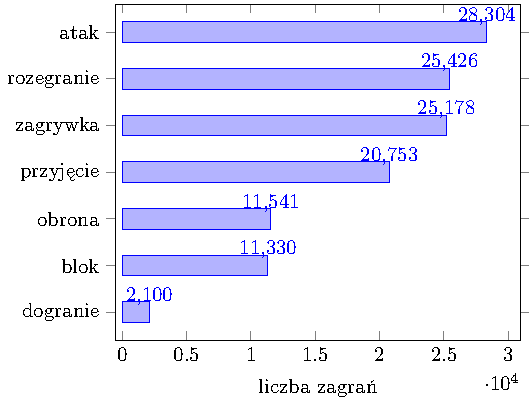
\includegraphics{zagrania}
\caption{Liczba zapisanych w~bazie danych zagrań poszczególnych rodzajów.}
\label{fig:zagrania}
\end{figure}

Również nierównomierna jest liczba zagrań wykonanych przez zawodników występujących na różnych pozycjach oraz w~różnych zespołach. W~tablicy \ref{tab:liczbaZagranRozegranie} przedstawiono dziesięciu zawodników z~największą liczbą rozegrań zapisanych w~bazie danych wraz z~odpowiadającą im liczbą zagrań. Każdy z~tych dziesięciu zawodników grał w~sezonie 2019/2020 w~innej drużynie Krispol 1. Ligi. Świadczy to o~tym, że w~przypadku pozycji rozgrywającego, których w~zespole jest dwóch, występuje podział na zawodnika podstawowego (grającego zdecydowaną większość akcji) i~rezerwowego. Tak jak wspomniano wcześniej to na analizę rozegrania poświęca się najwięcej czasu, w~związku z~czym najdokładniej rozpracowywuje się grę jednego zawodnika z~drużyny - podstawowego rozgrywającego.

\begin{table}
\centering
\caption{Dziesięciu zawodników z~największą liczbą rozegrań zapisanych w~bazie danych wraz z~odpowiadającą im liczbą zagrań.}
\label{tab:liczbaZagranRozegranie}
\begin{tabular}{lrl}
	\toprule
	{inicjały} & {liczba rozegrań} & {zespół}                         \\
	\midrule
	     M. M.       &              1603 & MCKiS Jaworzno                   \\
	     J. N.       &              1535 & KFC Gwardia Wrocław              \\
	     J. D.       &              1496 & SMS PZPS I Spała                 \\
	     B. N.       &              1372 & Lechia Tomaszów Mazowiecki       \\
	     P. A.       &              1292 & Exact Systems Norwid Częstochowa \\
	     P. S.       &              1278 & Stal Nysa S.A.                   \\
	     J. M.       &              1183 & BBTS Bielsko-Biała               \\
	     K. J.       &              1172 & AZS AGH Kraków                   \\
	     K. A.       &              1106 & SPS Chrobry Głogów               \\
	    K. D.       &              1033 & LUK Politechnika Lublin          \\
	\bottomrule
\end{tabular}
\end{table}

W przypadku rozegrania analiza została przeprowadzona dla dwóch atrybutów decyzyjnych: kierunku rozegrania oraz zawodnika, do którego została wystawiona piłka. W~przypadku kierunku rozegrania dane klasyfikowane są do pięciu klas decyzyjnych:
\begin{itemize}
\item F -- wystawy na lewe skrzydło (od ang. \ang{front}),
\item B -- wystawy na prawe skrzydło (od ang. \ang{back}),
\item C -- wystawy na środek siatki w~pierwszej linii (od ang. \ang{centre}),
\item P -- wystawy na środek siatki w~drugiej linii (od ang. \ang{pipe}),
\item S -- ataki rozgrywających z~drugiej piłki (od ang. \ang{setter}).
\end{itemize}

Liczba wystaw należących do każdej z~tych klas jest inna, co wynika nie tylko z~wyborów rozgrywających, ale przede wszystkim specyfiki tej dyscypliny sportu. Przykładowo ataki ze środka siatki w~pierwszej linii są możliwe jedynie zwykle tylko przy pozytywnym przyjęciu piłki lub dograniu piłki do siatki w~kontrze. Zwykle jednak około 50\% przyjęć i~75\% kontrataków wymusza na rozgrywającym wystawę piłki na któreś ze skrzydeł. Zdecydowanie najrzadziej natomiast rozgrywający ma możliwośc zaatakowania z~drugiej piłki. Ten nierówny rozkład kierunków wystaw widoczny jest w~tablicy \ref{tab:rozkladWystaw}.

\begin{table}
\centering
\caption{Rozkład poszczególnych kierunków wszystkich rozegrań piłki zapisanych w~bazie danych z~niepustą wartością atrybutu kierunku rozegrania.}
\label{tab:rozkladWystaw}
\begin{tabular}{lrr}
	\toprule
	kierunek & liczba & odsetek [\%] \\
	\midrule
	F        &   9889 &         40,4 \\
	B        &   7895 &         32,2 \\
	C        &   4633 &         18,9 \\
	P        &   1761 &          7,1 \\
	S        &    295 &          1,2 \\
	\bottomrule
\end{tabular}
\end{table}
Wystawy na lewe skrzydło wraz z~wystawami na prawe skrzydło stanowią ponad 72\% wszystkich wystaw, a~wystawy pipe wraz z~atakami rozgrywających z~drugiej piłki stanowią już zaledwie nieco ponad 8\%. Sumując liczbę rozegrań dla każdego z~kierunków nie otrzyma się liczby rozegrań przedstawionej na rysunku \ref{fig:zagrania}, jednak pominięte zostały wystawy bez wartości atrybutu kierunku rozegrania, na które składają się głównie błędy własne rozgrywających. Takich akcji w~analizowanej bazie danych było 953, czyli ponad 3 razy więcej niż ataków rozgrywających.

Przy analizie, do którego zawodnika została wystawiona piłka, liczba klas decyzyjnych jest równa liczbie zawodników w~danej drużynie, którzy wykonali atak z~przynajmniej jednej wystawy od analizowanego rozgrywającego. Drużyny dysponują zwykle 14-osobowymi składami, w~których znajduje się dwóch zawodników rozgrywających oraz dwóch zawodników libero, w~związku z~czym klas decyzyjnych w~przypadku takiej analizy dla każdego z~rozgrywających jest około 11 (10 zawodników atakujących + klasa decyzyjna ataków własnych analizowanego rozgrywającego). Liczba klas decyzyjnych nie musi być jednak równa 11, gdyż nie wszyscy zawodnicy atakujący dostają szansę gry nawet w~chociaż jednym spotkaniu w~sezonie, a~w~niektórych drużynach pojawiają się w~trakcie sezonu również kolejni nowi zawodnicy. Liczba wystaw do każdego z~zawodników zależna jest od kilku czynników takich jak: liczba wystąpień zawodnika wykonującego ataki w~pierwszym składzie, jego pozycja na boisku, a~także czy dany zawodnik stanowi o~sile ofensywnej drużyny, czy też ma spełniać w~niej inne role, jak na przykład przyjęcie, blok, obrona. 

\begin{table}
\centering
\caption{Rozkład liczby ataków poszczególnych zawodników drużyny MCKiS Jaworzno po wystawach zawodnika z~największą liczbą wystaw w~bazie danych.}
\label{tab:liczbaAtakowJaworzno}
\begin{tabular}{lrl}
\toprule
{inicjały} & {pozycja} & {liczba ataków} \\ 
\midrule
K.D. & przyjmujący & 275 \\
B.K. & atakujący & 218 \\ 
K.S. & środkowy & 211 \\ 
T.P. & przyjmujący & 192 \\ 
J.G. & przyjmujący & 183 \\ 
M.P. & środkowy & 134 \\ 
M.M. & rozgrywający & 59 \\ 
M.P. & środkowy & 26 \\ 
P.Ż. & środkowy & 23 \\
M.B. & przyjmujący & 13 \\ 
\bottomrule
\end{tabular}
\end{table}

Przykładem jest rozkład liczby ataków poszczególnych zawodników po wystawach zawodnika z~największą liczbą wystaw w~bazie danych, przedstawiony w~tablicy \ref{tab:liczbaAtakowJaworzno}. Najwięcej ataków ma zawodnik przyjmujący, który w~niemal każdym spotkaniu występował w~podstawowym składzie i~który zdobył najwięcej punktów w~swojej drużynie przez cały sezon. Na kolejnych pozycjach znajduje się dwóch zawodników grających na pozycji atakującego. Ostatnie 3 miejsca w~tym rozkładzie stanowią zawodnicy rezerwowi, z~czego najmniej ataków ma zawodnik, który najczęściej wchodził na boisku w~celu pomocy w~przyjęciu. 

\begin{table}
\centering
\caption{Dziesięciu zawodników z~największą liczbą ataków zapisanych w~bazie danych, wraz z~odpowiadającą im liczbą zagrań.}
\label{tab:liczbaZagranAtak}
\begin{tabular}{lrrl}
\toprule
{inicjały} & {pozycja} & {liczba ataków} & {zespół} \\
\midrule
D.W. & atakujący & 673 & LUK Politechnika Lublin \\
P.K. & atakujący & 642 & SMS PZPS I Spała \\ 
M.G. & przyjmujący & 574 & SMS PZPS I Spała \\ 
P.R. & przyjmujący & 560 & LUK Politechnika Lublin \\ 
K.D. & przyjmujący & 535 & MCKiS Jaworzno \\
M.P. & atakujący & 527 & ES Norwid Częstochowa \\ 
M.G. & atakujący & 515 & KFC Gwardia Wrocław \\
D.G. & atakujący & 511 & AZS AGH Kraków \\ 
Ł.L. & przyjmujący & 504 & KFC Gwardia Wrocław \\ 
M.B. & przyjmujący & 466 & Lechia Tomaszów Mazowiecki \\
\bottomrule
\end{tabular}
\end{table}

\begin{table}
\centering
\caption{Dziesięciu środkowych z~największą liczbą ataków zapisanych w~bazie danych, wraz z~odpowiadającą im liczbą zagrań.}
\label{tab:liczbaZagranAtakSrodkowi}
\begin{tabular}{lrl}
\toprule
{inicjały} & {liczba ataków} & {zespół} \\
\midrule
K.S. & 287 & MCKiS Jaworzno \\ 
A.O. & 215 & KFC Gwardia Wrocław \\ 
B.S. & 198 & KFC Gwardia Wrocław \\ 
J.M. & 192 & AZS AGH Kraków \\
M.P. & 187 & MCKiS Jaworzno \\ 
M.S. & 186 & Exact Systems Norwid Częstochowa \\ 
M.Z. & 184 & APP Krispol Września \\ 
Ł.U. & 182 & Exact Systems Norwid Częstochowa \\
H.W. & 179 & SPS Chrobry Głogów \\ 
A.H. & 176 & BBTS Bielsko-Biała \\
\bottomrule
\end{tabular}
\end{table}

Podobnie jak w~przypadku rozegrania w~tablicy \ref{tab:liczbaZagranAtak} przedstawiono dziesięciu zawodników z~największą liczbą ataków zapisanych w~bazie danych, wraz z~odpowiadającą im liczbą zagrań. Porównując z~tablicą rozgrywających (tab.~\ref{tab:liczbaZagranRozegranie}) liczba ataków jest ponad dwukrotnie mniejsza. Wynika to z~faktu, że atak w~każdej z~drużyn rozkłada się pomiędzy wspomnianymi około dzisięcioma zawodnikami, a~nie jak w~przypadku rozegrania, gdzie jeden rozgrywający i~ewentualnie jego zmiennik odpowiadają za zdecydowaną większość rozegrań swojej drużyny w~meczu. 

W przypadku najliczniej atakujących zawodników znajdują się zawodnicy z~tych samych drużyn. Są to zawodnicy z~drużyn, w~przypadku których gra ofensywna była rozłożona mniej równomiernie. Cała dziesiątka zawodników z~największą liczbą ataków to natomiast zawodnicy skrzydłowi. Z~tego też powodu osobno przeanalizowani zostali zawodnicy środkowi (tab.~\ref{tab:liczbaZagranAtakSrodkowi}). W~ich przypadku również znajdują się pary zawodników z~tych samych drużyn. Reprezentują oni trzy drużyny, które w~meczach wczytanych do bazy wyprowadziły najwięcej ataków ze środka siatki. Łącznie jednak ataków środkowych zanotowano ponad 4 razy mniej niż ataków skrzydłowych - odpowiednio 5063 i~22593.

Dziesięciu zawodników z~największą liczbą przyjęć zapisanych w~bazie danych zostało przedstawionych w~tablicy \ref{tab:liczbaZagranPrzyjecie}. W~tym przypadku są to zazwyczaj zawodnicy przyjmujący oraz libero, którzy najczęściej byli wybierani jako cel zagrywki drużyny przeciwnej. Mogło to wynikać z~faktu, że jakość przyjęcia tych zawodników była niższa od pozostałych zawodników tej drużyny lub w~przypadku zawodników na pozycji przyjmującego zagrywki były posyłane w~ich stronę, by utrudnić im późniejsze wykonanie ataku. To ostatnie potwierdza również fakt, iż czterech z~pięciu przyjmujących występujących w~tablicy przedstawiającej zawodników z~największą liczbą ataków znajduje się również w~tablicy przedstawiającej zawodników z~największą liczbą przyjęć.

\begin{table}
\centering
\caption{Dziesięciu zawodników z~największą liczbą przyjęć zapisanych w~bazie danych, wraz z~odpowiadającą im liczbą zagrań.}
\label{tab:liczbaZagranPrzyjecie}
\begin{tabular}{lrrl}
\hline
\toprule
{inicjały} & {pozycja} & {liczba przyjęć} & {zespół} \\
\midrule
M.G. & przyjmujący & 580 & SMS PZPS I Spała \\ 
M.K. & libero & 580 & ES Norwid Częstochowa \\ 
K.D. & przyjmujący & 529 & MCKiS Jaworzno  \\ 
Ł.K. & przyjmujący & 526 & ES Norwid Częstochowa \\ 
Ł.L. & przyjmujący & 485 & KFC Gwardia Wrocław \\ 
J.C. & przyjmujący & 470 & SMS PZPS I Spała \\
K.G. & przyjmujący & 468 & KFC Gwardia Wrocław \\ 
M.B. & przyjmujący & 455 & Lechia Tomaszów Mazowiecki \\
K.G. & przyjmujący & 450 & KPS Siedlce \\ 
D.P. & libero & 448 & ZAKSA Strzelce Opolskie \\
\bottomrule 
\end{tabular}
\end{table}

\subsection{Przygotowanie danych}
\label{roz:przygotowanie-danych}

Aplikacja pozwala na wczytywanie danych z~opisanych w~rozdziale \ref{roz:analiza-kodu} plików o~rozszerzeniu \texttt{dvw}. Te następnie są zapisywane do bazy danych składającej się z~pięciu tabel: 
\begin{itemize}
\item meczów,
\item drużyn,
\item zawodników,
\item ustawień,
\item zagrań.
\end{itemize}
W pierwszych trzech tabelach przechowywane są informacje o~wczytanych meczach, drużynach oraz ich zawodnikach. W~tabeli ustawień zapisane są informacje o~id zawodników znajdujących się na każdej z~sześciu pozycji w~obu drużynach w~każdej kolejnej akcji w~meczu. Wszystkie dane dotyczące wykonanych zagrań w~meczu znajdują się natomiast w~tabeli zagrań. To na podstawie danych zawartych w~tej tabeli przeprowadzane są wszystkie późniejsze operacje eksploracji danych. 

Tabela zagrań składa się z~aż 38 atrybutów. Każdy rekord w~tej tabeli, oprócz własnego klucza głównego, posiada klucze obce z~informacjami o~id zawodnika i~meczu, którego dotyczy dane zagranie, tworząc w~ten sposób relacje z~tabelami zawodników oraz meczów. Pozostałe 35 atrybutów to natomiast wszelkie informacje możliwe do uzyskania z~kolejnych wierszy wczytywanych plików. Oprócz informacji otrzymywanych bezpośrednio na podstawie pierwszych 15 znaków zapisu kodu akcji przechowywane są również informacje o~stanie meczu (liczba punktów obu drużyn, numer i~faza seta, czas meczu, ustawienie obu drużyn), a~także informacje uzyskane na podstawie wcześniejszych zagrań takie jak: kierunek poprzedniej wystawy, jakość przyjęcia oraz wystawy mające wpływ na późniejszy atak zawodnika, liczba ataków w~danej akcji, czy też liczba ataków zawodnika w~meczu. 

Lista wszystkich atrybutów w~tabeli zagrań:
\begin{itemize}
\item \texttt{id} -- klucz główny tabeli
\item \texttt{gameID} -- klucz obcy, id w~tabeli meczów
\item \texttt{playerID} -- klucz obcy, id w~tabeli zawodników
\item \texttt{nr} -- numer akcji w~meczu
\item \texttt{setNr} -- numer seta w~meczu
\item \texttt{hPoints} -- liczba punktów zespołu gospodarzy
\item \texttt{vPoints} -- liczba punktów zespołu gości
\item \texttt{setPhase} -- faza seta (5 klas: ,,0'' -- różnica punktowa między drużynami > 6, ,,1'' -- początek seta (do 8 punktów zdobytych przez jedną z~drużyn), ,,2'' -- środek seta (do 20 punktów zdobytych przez jedną z~drużyn), ,,3'' -- końcówka seta (do 24 punktów zdobytych przez jedną z~drużyn), ,,4'' -- gra na przewagi)
\item \texttt{serveSide} -- strona zagrywająca (gospodarze: ,,*'', goście: ,,a'')
\item \texttt{actionSide\footnote{\label{codeSyntax}Opis atrybutów pochodzących bezpośrednio z~zapisu kodu akcji opisanego w~rozdziale \ref{roz:analiza-kodu}}} -- strona wykonująca zagranie
\item \texttt{skill\textsuperscript{\ref{codeSyntax}}} -- rodzaj zagrania
\item \texttt{type\textsuperscript{\ref{codeSyntax}}} -- typ zagrania
\item \texttt{quality\textsuperscript{\ref{codeSyntax}}} -- jakość zagrania
\item \texttt{setterCmb\textsuperscript{\ref{codeSyntax}}} -- ruch rozgrywającego
\item \texttt{attackCmb\textsuperscript{\ref{codeSyntax}}} -- kombinacja ataku
\item \texttt{trg\textsuperscript{\ref{codeSyntax}}} -- kierunek rozegrania
\item \texttt{startZone\textsuperscript{\ref{codeSyntax}}} -- strefa początkowa zagrania
\item \texttt{endZone\textsuperscript{\ref{codeSyntax}}} -- strefa końcowa zagrania
\item \texttt{endZoneExt\textsuperscript{\ref{codeSyntax}}} -- rozszerzona strefa końcowa zagrania
\item \texttt{skillType\textsuperscript{\ref{codeSyntax}}} -- dodatkowa informacja o~typie umiejętności dla danego typu zagrania
\item \texttt{players\textsuperscript{\ref{codeSyntax}}} -- informacja o~liczbie zawodników (przede wszystkim w~bloku)
\item \texttt{special\textsuperscript{\ref{codeSyntax}}} -- dodatkowe pole wykorzystywane przez niektórych statystyków
\item \texttt{time} -- przedział czasu trwającego meczu (4 klasy: ,,$<15$min'', ,,$(15\,$min$, 1\,$h$\rangle$'', ,,$(1\,$h$, 2\,$h$\rangle$'', ,,$>2\,$h'')
\item \texttt{hSetterPosition} -- ustawienie zespołu gospodarzy
\item \texttt{vSetterPosition} -- ustawienie zespołu gości  
\item \texttt{recDefQ} -- jakość przyjęcia/obrony
\item \texttt{setQ} -- jakość rozegrania
\item \texttt{setPosition} -- strefa rozegrania
\item \texttt{setZone} -- strefa, do której rozegrano piłkę
\item \texttt{attackDirection} -- kierunek ataku (w lewo, w~środek, w~prawo)
\item \texttt{lastSetTrg} -- kierunek poprzedniej wystawy
\item \texttt{lastSetZone} -- strefa, do której poprzednio rozegrano piłkę
\item \texttt{recPlayerID} -- id zawodnika przyjmującego zagrywkę
\item \texttt{setToWhichPlayerID} -- id zawodnika, do którego rozegrana została piłka
\item \texttt{attackAttemt} -- który atak w~akcji
\item \texttt{playerAttackAttempt} -- który atak zawodnika w~meczu
\item \texttt{sideOutAttempt} -- która próba zrobienia przez drużynę przejścia
\item \texttt{point} -- która drużyna zdobyła punkt w~akcji
\end{itemize}

Pierwszym pomysłem na zbadanie zależności we wczytanych danych do bazy była próba ich grupowania. W~tym celu przetestowano działanie algorytmów $k$-średnich (ang. \ang{k-means}) oraz samoorganizującej sieci Kohonena \cite{bib:wekaSOM} dla danych dotyczących zagrań całej drużyny oraz pojedynczych zawodników. Testy te jednak ze względu na brak otrzymanych jakichkolwiek interesujących wyników zakończyły się niepowodzeniem. Potwierdziły one jednak fakt, że znajdowanie zależności w~grze poszczególnych zawodników w~meczach siatkarskich nie należy do łatwych zadań.

Po próbie grupowania przeprowadzone zostały testy wykorzystujące algorytmy do odkrywania klasyfikacji oraz asocjacji. Testy te pozwoliły zauważyć, że pewne atrybuty są mocno od siebie zależne. Niektóre z~nich miały nawet relacje tożsamościowe, gdyż przykładowo zawsze gdy wystawa kierowana była do czwartej strefy (zapisanej jako wartość atrybutu strefy końcowej zagrania), czyli do pierwszej linii na lewe skrzydło, atrybut kierunku wystawy miał wartość ,,F'' rozumiany właśnie jako wystawa na lewe skrzydło. Takich zależności było zdecydowanie więcej, przez co należało wybrać atrybuty, które mogą być wspólnie analizowane. 

Ostatecznie w~przeprowadzonych w~pracy badaniach analizie poddano trzy główne zagrania analizowane zwykle przez sztaby trenerskie: rozegranie, atak oraz przyjęcie. Dla każdego z~tych rodzajów zagrań, na podstawie konsultacji ze statystykiem siatkarskim, wybrane zostały podzbiory atrybutów z~tabeli zagrań oraz odpowiednie klasy decyzyjne, pozwalające uzyskać najbardziej interesujące dla sztabów trenerskich wyniki. Do analizy wszystkich trzech rodzajów zagrań wykorzystane zostały atrybuty strefy początkowej oraz strefy końcowej zagrania, które dla każdego rodzaju zagrania oznacza co innego, a~mianowicie:
\begin{itemize}
\item dla rozegrania:
\begin{itemize}
\item strefa początkowa -- strefa przyjęcia/obrony
\item strefa końcowa -- strefa rozegrania
\end{itemize}
\item dla ataku:
\begin{itemize}
\item strefa początkowa -- strefa rozegrania
\item strefa końcowa -- strefa ataku
\end{itemize}
\item dla przyjęcia:
\begin{itemize}
\item strefa początkowa -- strefa zagrywki
\item strefa końcowa -- strefa przyjęcia
\end{itemize}
\end{itemize}
Dla każdego rodzaju zagrania wykorzystywane są także atrybuty dotyczące aktualnego stanu meczu, czyli: 
\begin{itemize}
\item numeru seta,
\item fazy seta,
\item czasu meczu,
\item liczby prób zrobienia przez drużynę przejścia,
\item ustawienia zespołu gospodarzy,
\item ustawienia zespołu gości.
\end{itemize}
Oprócz tego dla poszczególnych rodzajów zagrań wybrane zostały również następujące atrybuty:
\begin{itemize}
\item dla rozegrania:
\begin{itemize}
\item ruch rozgrywającego
\item jakość przyjęcia/obrony
\item kierunek poprzedniej wystawy
\item która próba ataku w~akcji
\item przyjmujący
\end{itemize}
\item dla ataku:
\begin{itemize}
\item rodzaj wystawy
\item rodzaj ataku
\item kombinacja ataku
\item jakość wystawy
\item która próba ataku w~akcji
\item która próba ataku zawodnika w~meczu
\item liczba zawodników w~bloku
\end{itemize}
\item dla przyjęcia:
\begin{itemize}
\item rodzaj zagrywki
\end{itemize}
\end{itemize}
Stworzony program umożliwia wybór wszystkich możliwych, lub tylko wybranych przez użytkownika atrybutów do analizy danego rodzaju zagrania. Wybranymi możliwymi atrybutami decyzyjnymi zostały natomiast:
\begin{itemize}
\item dla rozegrania:
\begin{itemize}
\item kierunek wystawy
\item do jakiego zawodnika wystawa
\item do jakiej strefy wystawa
\end{itemize}
\item dla ataku:
\begin{itemize}
\item kierunek ataku
\item strona boiska w~jaką nastąpił atak (lewa, prawa, w~środek)
\end{itemize}
\item dla przyjęcia:
\begin{itemize}
\item jakość przyjęcia
\end{itemize}
\end{itemize}

Każde z~zagrań nie jest analizowane jednak dla całości danych wczytanych do bazy, a~jedynie danych dotyczących zagrań pojedynczych zawodników. Dla rozgrywających możliwe jest badanie jedynie ich rozegrania, dla atakujących oraz środkowych ich ataków, dla libero jedynie ich przyjęcia, natomiast dla przyjmujących badane są zarówno ich przyjęcia jak i~ataki. Analiowane dane mogą pochodzić z~dowolnej, wybranej przez użytkownika listy meczów.

\subsection{Analiza wartości oczekiwanych dla rozegrania}
Otrzymane wyniki dokładności klasyfikacji, zarówno dla drzew decyzyjnych jak i~reguł asocjacyjnych, zostały porównane dodatkowo w~pracy z~wartościami oczekiwanymi. Wartość oczekiwana dla zmiennych dyskretnych wyrażana jest wzorem:
\begin{equation}
\label{wz:warocz}
E(X) = \sum_{i=1}^{n} x_i p_i
\end{equation}
gdzie:
\begin{align*}
	X	&- \text{zmienna losowa o~rozkładzie dyskretnym}\\
	n	&- \text{liczba wartości przyjmowanych przez X}\\
	x_i	&- \text{$i$-ta wartość przyjmowana przez X}\\
	p_i &- \text{prawdopodobieństwo wystąpienia w~X $i$-tej wartości}
\end{align*}
Wartości te określają spodziewany wynik doświadczenia losowego, czyli w~tym przypadku próby klasyfikacji badanych zagrań zgodnie z~prawdopodobieństem występowania poszczególnych klas decyzyjnych. W~związku z~tym liczbą wartości przyjmowanych przez zmienną losową będzie liczba występujących klas, natomiast zarówno wartości przyjmowane przez zmienną losową jak i~estymacja prawdopodobieństwa ich występowania określać będzie stosunek obserwacji z~danej klasy do wszystkich obserwacji.

W tablicy \ref{tab:prawdopodobienstwoRozegranie} przedstawiono wyliczone wartości oczekiwane dla dziesięciu zawodników z~największą liczbą rozegrań, przy analizie kierunku rozegrania. Zauważyć można, że mimo występowania pięciu klas decyzyjnych, uzyskiwane wyniki wynoszą około 30\%. W~przypadku w~miarę równego rozkładu każdej z~klas decyzyjnych wynik ten powinien wynieść około 20\%. Wyniki te jednak są tym wyższe, im mniej zróżnicowana jest gra rozgrywającego. Również ze względu na małą liczbę danych z~atakami rozgrywających z~drugiej piłki oraz wystaw na środek siatki w~drugiej linii dużo trudniej jest znaleźć odpowiednie warunki pozwalające przewidzieć i~zaklasyfikować te zagrania do właściwych klas.

\begin{table}
\centering
\caption{Wartości oczekiwane dokładności klasyfikacji dla dziesięciu zawodników z~największą liczbą rozegrań zapisanych w~bazie danych, przy analizie kierunku rozegrania.}
\label{tab:prawdopodobienstwoRozegranie}
\begin{tabular}{rc}
\toprule
inicjały & wartość oczekiwana \\ \midrule
M.M. & 27,324 \\ 
J.N. & 28,622 \\ 
J.D. & 35,672 \\ 
B.N. & 33,196 \\ 
P.A. & 28,457 \\ 
P.S. & 26,513 \\ 
J.M. & 28,863 \\ 
K.J. & 29,163 \\ 
K.A. & 28,764 \\ 
K.D. & 32,314\\ 
\midrule
\textbf{średnia} & \textbf{29,889} \\ 
 \bottomrule
\end{tabular}
\end{table}

Im gra ofensywna zespołu oparta jest na większej liczbie zawodników, tym niższa jest wartość oczekiwana dokładności klasyfikacji, przy analizie do jakiego zawodnika nastąpi rozegranie (tab.~\ref{tab:prawdopodobienstwoRozegranieZawodnicy}). W~przypadku rozgrywających, dla których wynik ten jest wyższy niż 20\% za atak odpowiedzialnych było głownie 2-3 zawodników. W~przypadku zespołu SMS PZPS I Spała, gdzie podstawowym rozgrywającym był J.D. dwóch zawodników wykonało 50,6\% wszystkich ataków w~drużynie, a~po doliczeniu ataków trzeciego zawodnika najczęściej atakującego łącznie wykonali oni aż 68,2\% wszystkich ataków. Podobnie w~przypadku zespołu AZS AGH Kraków, gdzie podstawowym rozgrywającym był K.J., dwóch zawodników najczęściej atakujących wykonało 54,5\% wszystkich ataków wykonanych przez cały sezon w~tej drużynie. Trzeci najczęściej atakujący zawodnik tej drużyny wykonał już jednak tylko 13,1\% ataków, w~związku z~czym łącznie to trzech zawodników drużyny SMS PZPS I Spała wykonało wyższy odsetek wszystkich ataków w~swojej drużynie. Dla porównania w~przypadku zaprezentowanego w~tablicy \ref{tab:liczbaAtakowJaworzno} rozkładu liczby ataków zawodników drużyny MCKiS Jaworzno po wystawach rozgrywającego M.M. dwóch najczęściej atakujących zawodników po jego wystawach wykonało 32,5\% ataków, a~po dodaniu ataków trzeciego najczęściej atakującego zawodnika wykonali oni łącznie w~trójkę mniej niż 50\% ataków po jego wystawach, dokładnie 46,4\%. Przekłada się to na wynik wartości oczekiwanej dokładności klasyfikacji, która dla zawodnika M.M. wynosi zaledwie 12,3. Wyniki te dla wszystkich rozgrywających są jednak blisko dwukrotnie niższe niż w~przypadku analizy kierunku rozegrania. 

W eksperymentach przedstawionych w~rozdziałach \ref{roz:klasyfikacja-drzewa} oraz \ref{roz:klasyfikacja-reguly} zbadane zostało czy wyższe wyniki wartości oczekiwanych dla poszczególnych zawodników przy analizie kierunku rozegrania przekładają się również na wyższe wyniki w~przypadku tych zawodników przy klasyfikacji z~wykorzystaniem drzew decyzyjnych oraz reguł asocjacyjnych.

\begin{table}
\centering
\caption{Wartości oczekiwane dokładności klasyfikacji dla dziesięciu zawodników z~największą liczbą rozegrań zapisanych w~bazie danych, przy analizie do jakiego zawodnika następuje rozegranie.}
\label{tab:prawdopodobienstwoRozegranieZawodnicy}
\begin{tabular}{rc}
\toprule
{inicjały} & {wartość oczekiwana} \\
\midrule
M.M. & 12,825 \\ 
J.N. & 17,190 \\ 
J.D. & 20,950 \\ 
B.N. & 14,907 \\ 
P.A. & 15,425 \\ 
P.S. & 15,689 \\
J.M. & 15,636 \\
K.J. & 20,001 \\
K.A. & 12,391 \\ 
K.D. & 19,939 \\ 
\midrule
\textbf{średnia} & \textbf{16,495} \\ 
\bottomrule
\end{tabular}
\end{table}

\section{Miary}

Miarą użytą w~celu porównania otrzymanych wyników klasyfikacji zagrań jest opisana w~rozdziale \ref{roz:klasyfikacja} dokładność klasyfikacji.
We wszystkich zaprezentowanych w~pracy wynikach badań dokładność klasyfikacji została przedstawiona w~postaci wartości procentowych.

Ze względu na występującą nierównomierną dystrybucję klas dla kilku ciekawszych wyników otrzymanych dla klasyfikacji z~wykorzystaniem drzew decyzyjnych porównano również wyniki miary $F_1$, będącej średnią harmoniczną precyzji i~czułości:
\begin{equation}
F_1 = 2 \cdot \frac{pr \cdot re}{pr + re}
\end{equation}
\begin{equation}
pr = \frac{t_p}{t_p + f_p}
\end{equation}
\begin{equation}
re = \frac{t_p}{t_p + f_n}
\end{equation}

gdzie:
\begin{align*}
	pr	&- \text{precyzja}\\
	re	&- \text{czułość}\\
	t_p &- \text{liczba obserwacji dobrze przypisanych do analizowanej klasy}\\
    f_p &- \text{liczba obserwacji błędnie przypisanych do analizowanej klasy}\\
    f_n &- \text{liczba obserwacji analizowanej klasy przypisanych błędnie do innej klasy}
\end{align*} 
Miara ta pozwala pozwala zaobserwować na przykład, czy stworzony model, dający najlepsze wyniki jeśli chodzi o~dokładność klasyfikacji, dobrze radzi sobie z~klasyfikacją obserwacji dla mniej licznych klas. Wyniki tej miary osiągają wartości w~przedziale od 0 do 1. Im wyższa uzyskana wartość dla danej klasy tym lepiej klasyfikator radzi sobie z~klasyfikacją obserwacji należących do tej klasy.


\section{Metodyka badań}
\label{roz:metodyka}

Przeprowadzone badania objęły analizę istotności poszczególnych atrybutów dla każdego z~trzech rodzajów zagrań: przyjęcia, rozegrania oraz ataku, a~także analizę wyników klasyfikacji przeprowadzoną tylko dla akcji rozegrania. W~tym celu wykorzystano opisane w~rozdziale \ref{roz:algorytmy} metody eksploracji danych: klasyfikację z~użyciem drzew decyzyjnych (algorytm C4.5) oraz klasyfikację reguł asocjacyjnych (algorytm CBA). Przeprowadzona analiza objęła wyniki dla pojedynczych zawodników oraz uzyskanych średnich dla 10 zawodników z~największą liczbą zagrań.

Zbadane zostały również wyniki uzyskane w~zależności od wartości parametrów wyszukiwania reguł asocjacyjnych oraz budowy drzew decyzyjnych\footnote{\label{parametry} Parametry te zarówno dla drzew decyzyjnych jak i~reguł asocjacyjnych zostały nazwane w~programie jako \ang{support} (minimalne wsparcie reguł, minimalna liczba instancji w~liściach drzew) oraz \ang{confidence} (minimalna ufność reguł, poziom ufności CF)}. W~przypadku reguł asocjacyjnych są to parametry minimalnego wsparcia i~minimalnej ufności reguł, natomiast w~przypadku drzew decyzyjnych minimalnej liczby instancji w~liściach oraz poziom ufności CF (ang. \ang{confidence factor}), używanego do przycinania drzewa \cite{bib:confidenceFactor}. Wartość parametru poziomu ufności jest rozumiana jako maksymalny szacunkowy błąd klasyfikacji, obliczany dla danego węzła drzewa. Im mniejsza wartość parametru tym ostrzejsze przycięcie drzewa.

Oprócz tego porównano wyniki uzyskane zarówno z~jak i~bez włączonej selekcji atrybutów, a~także w~zależności od liczby analizowanych meczów oraz przeciwników. W~przypadku włączonej selekcji atrybutów podawana jest minimalna wartość miary przyrostu informacji. Po zastosowaniu selekcji atrybutów dane, na podstawie których przeprowadzane są badania zostają obcięte tylko do atrybutów, których miara przyrostu informacji jest wyższa od podanej w~wywołaniu minimalnej wartości.

W celu wykonania badań dla różnych zawodników oraz różnych ustawień parametrów w~aplikacji zaimplementowano możliwość wywołania w~pętli badań dla wybranych zawodników oraz automatyczną inkrementacją parametrów przeszukiwań. Dla drzew decyzyjnych parametr minimalnej liczby instancji w~liściach inkrementowany był w~przedziale od 2 do 25 co 1, natomiast parametr poziomu ufności od 0,01 do 0,5 co 0,01. Dla reguł asocjacyjnych parametr minimalnego wsparcia reguł inkrementowany był w~przedziale od 5 do 25 co 5, a~parametr minimalnej ufności reguł od 0,5 do 1 co 0,1. Chcąc przeprowadzić badania dla reguł asocjacyjnych z~takim samym krokiem inkrementacji jak dla drzew decyzyjnych, łączny czas badań bez selekcji atrybutów dla zaledwie dwóch zawodników wyniósł ponad 12 i~pół godziny, gdzie dla porównania czas badań dla 10 zawodników bez selekcji atrybutów z~wykorzystaniem drzew decyzyjnych wyniósł nieco ponad 7 minut. Wyniki uzyskane w~ten sposób zostały omówione w~eksperymencie sprawdzającym zależność wyników klasyfikacji od wartości parametrów (\ref{roz:eks-parametry}), jednak po przeanalizowaniu ich i~dojściu do wniosku, że nie dają zysku (w postaci znalezienia ciekawych zależności) proporcjonalnego do ilości poświęconego na tego typu badania czasu, do wyliczenia wartości średnich postanowiono zastosować większy niż w~przypadku drzew decyzyjnych krok inkrementacji parametrów użytych w~badaniach. 

Zbiory otrzymywanych wyników zostały automatycznie zapisywane przez program do plików o~rozszerzeniu ,,csv''. Wyniki te zostały następnie zaimportowane do arkuszy kalkulacyjnych, na podstawie których sporządzono zamieszczone w~pracy tabele oraz wykresy. 

\section{Ranking istotności atrybutów}
Celem tego eksperymentu było znalezenie atrybutów mających największe znaczenie na wynik klasy decyzyjnej, dla każdego z~trzech analizowanych rodzajów zagrań. W~tym celu, za pomocą miary przyrostu informacji (wzór \ref{wz:przyrostinf}), wyliczone zostały wartości oceny atrybutów wyselekcjonowanych do analizy każdego z~analizowanych rodzajów zagrań. Dla każdego z~rodzajów zagrań analiza została przeprowadzona dla wyszukanych wcześniej dziesięciu zawodników z~największą liczbą zagrań tego typu. Na podstawie tych dziesięciu wyników wyliczone zostały również średnie tworzące rankingi atrybutów dla każdego z~rodzajów zagrań. Przeanalizowane zostały wyniki uzyskane zarówno dla średnich jak i~pojedynczych zawodników, porównując również oceny wartości tych samych atrybutów w~zależności od wybranego atrybutu decyzyjnego. W~przypadku rozegrania oraz ataku oprócz przeprowadzonej analizy dla wszystkich akcji sprawdzono również wartości atrybutów przy analizie samych akcji po przyjęciu i~samych akcji w~kontrataku. Dla rozegrania analizując akcje po przyjęciu pojawia się dodatkowy atrybut ,,Przyjmujący'', oznaczający zawodnika, który przyjmował piłkę. W~przypadku atrybutów ,,Jakość przyjęcia/obrony'' oraz ,,Strefa przyjęcia/obrony'' dla akcji po przyjęciu dotyczą one odpowiednio jakości i~strefy przyjęcia, natomiast dla kontrataków jakość i~strefy obrony. 

\subsection{Analiza rozegrania}
Przy analizie kierunku rozegrania (tab.~\ref{tab:atrybutyRKierunek}) najwyższe wartości osiągają atrybuty ,,Strefa rozegrania'', ,,Ruchy rozgrywającego'' oraz ,,Jakość przyjęcia/obrony''. Kolejny atrybut ,,Ustawienie (1-6)'' ma już średnią wartość oceny poniżej 0,05. Pozostałe natomiast mają średnia wartości niższe niż 0,02. Obecnie analiza statystyków odnośnie kierunku rozegrania opiera się właśnie na sprawdzeniu tych czterech pierwszych cech. Z~tych czterech cech najwięcej informacji przekazywanych zawodnikom jest jednak odnośnie tego w~jakim kierunku posyłane są piłki w~zależności od ustawienia zespołu. W~przypadku analizy kierunku rozegrania atrybuty ,,Strefa rozegrania'' i~,,Ruchy rozgrywającego'' mają jednak dwukrotnie wyższą średnią wartość oceny.

\begin{table}
\centering
\caption{Ocena istotności poszczególnych atrybutów przy analizie kierunku rozegrania.}
\label{tab:atrybutyRKierunek}
\begin{adjustbox}{angle=90}
\begin{tabular}{|l|c|c|c|c|c|c|c|c|c|c|c|}
\hline
\multirow{2}{*}{\textbf{nazwa atrybutu}} &
\multicolumn{10}{c|}{\textbf{inicjały rozgrywających z~największą liczbą wystaw}} & 
\multirow{2}{*}{\textbf{średnia}}\\
\cline{2-11} & \textbf{M.M.} & \textbf{J.N.} & \textbf{J.D.} & \textbf{B.N.} & \textbf{P.A.} & \textbf{P.S.} & \textbf{J.M.} & \textbf{K.J.} & \textbf{K.A.} & \textbf{K.D.} &\\
\hline
 Strefa rozegrania & \cellcolor{green}0,130 & \cellcolor{green}0,051 & \cellcolor{green}0,113 & 0,052 & 0,106 & 0,066 & \cellcolor{green}0,291 & 0,066 & 0,067 & \cellcolor{green}0,135 & \textbf{0,108} \\ \hline
 Ruchy rozgrywającego & 0,098 & 0,050 & 0,079 & \cellcolor{green}0,087 & \cellcolor{green}0,145 & \cellcolor{green}0,089 & 0,116 & 0,116 & \cellcolor{green}0,102 & 0,072 & \textbf{0,095} \\ \hline
 Jakość przyjęcia/obrony & 0,071 & 0,045 & 0,106 & 0,019 & 0,097 & 0,072 & 0,056 & \cellcolor{green}0,117 & 0,063 & 0,049 & \textbf{0,070} \\ \hline
 Ustawienie (1-6) & 0,087 & 0,045 & 0,036 & 0,048 & 0,036 & 0,036 & 0,050 & 0,050 & 0,051 & 0,037 & \textbf{0,048} \\ \hline
 Ustawienie przeciwnika (1-6) & 0,034 & 0,017 & 0,013 & 0,013 & 0,017 & 0,016 & 0,023 & 0,015 & 0,019 & 0,020 & \textbf{0,019} \\ \hline
 Strefa przyjęcia/obrony & 0,008 & 0,018 & 0,024 & 0,021 & 0,009 & 0,018 & 0,018 & 0,018 & 0,031 & 0,018 & \textbf{0,018} \\ \hline
 Który atak w~akcji & 0,014 & 0,013 & 0,015 & 0,020 & 0,010 & 0,018 & 0,019 & 0,012 & 0,006 & 0,030 & \textbf{0,016} \\ \hline
 Faza seta & 0,015 & 0,009 & 0,012 & 0,012 & 0,017 & 0,010 & 0,010 & 0,009 & 0,016 & 0,010 & \textbf{0,012} \\ \hline
 Kierunek poprzedniej wystawy & 0,008 & 0,008 & 0,011 & 0,005 & 0,008 & 0,008 & 0,017 & 0,009 & 0,014 & 0,018 & \textbf{0,011} \\ \hline
 Numer seta & 0,011 & 0,005 & 0,009 & 0,007 & 0,014 & 0,008 & 0,009 & 0,013 & 0,006 & 0,021 & \textbf{0,010} \\ \hline
 Czas meczu & 0,008 & 0,004 & 0,007 & 0,003 & 0,011 & 0,008 & 0,011 & 0,013 & 0,005 & 0,014 & \textbf{0,008} \\ \hline
 Która próba przejścia & 0,008 & 0,002 & 0,002 & 0,005 & 0,006 & 0,007 & 0,006 & 0,009 & 0,003 & 0,007 & \textbf{0,006} \\ \hline
\end{tabular}
\end{adjustbox}
\end{table}

Nie dla każdego z~zawodników jednak ten sam atrybut jest najistotniejszy. Przykładowo dla zawodników o~inicjałach P.S. oraz K.J. atrybut ,,Strefa rozegrania'', który uzyskał najwyższą średnią oceny dla dziesięciu zawodników, jest dopiero trzecim w~kolejności istotności atrybutem. Dla zawodnika K.J. najwyższą wartość oceny uzyskał, dopiero trzeci według średniej oceny, atrybut ,,Jakość przyjęcia/obrony''. Już na podstawie pierwszych wyników można więc wywnioskować, że istotność atrybutów dla każdego z~zawodników może być różna.  

Atrybut ,,Ustawienie (1-6)'', który miał dopiero czwartą średnią ocenę przy analizie kierunku rozegrania ma za to zdecydowanie najwyższą średnią wartość oceny w~przypadku analizy do jakiego zawodnika zostanie wystawiona piłka. Zarówno w~przedstawionych tablicach z~wynikami akcji po przyjęciu (tab.~\ref{tab:atrybutyRZawodnikPrzyjęcie}) oraz kontratakach (tab.~\ref{tab:atrybutyRZawodnikKontra}) średnia wartość oceny atrybutu ,,Ustawienie (1-6)'' wynosi ponad 0,3. Ponad sześciokrotnie wyższa wartość tego atrybutu przy analizie do jakiego zawodnika zostanie wystawiona piłka wynika z~faktu, że w~poszczególnych ustawieniach zwykle ci sami zawodnicy są rozpisani na tych samych pozycjach. W~każdym z~ustawień piłka wystawiana jest zwykle do zawodników znajdujących się w~tym ustawieniu w~pierwszej linii lub atakującego, który otrzymuje też sporo wystaw będąc w~drugiej linii. Sporadycznie wystawiane są jeszcze piłki na pipe'a. W~przypadku przyjmujących większość, a~w~przypadku środkowych w~zasadzie wszystkie rozegrane do nich piłki będą w~trzech z~sześciu ustawień, w~których to znajdują się oni w~pierwszej linii. W~związku z~tym dla każdego z~ustawień, przy analizie do jakiego zawodnika zostanie wystawiona piłka, klasami decyzyjnymi, które stanowią większość wszystkich analizowanych wystaw będą inne grupy zawodników otrzymujących piłki do ataku.

\begin{table}
\centering
\caption{Ocena istotności poszczególnych atrybutów przy analizie do jakiego zawodnika zostanie wystawiona piłka w~akcji po przyjęciu.}
\label{tab:atrybutyRZawodnikPrzyjęcie}
\begin{adjustbox}{angle=90}
\begin{tabular}{|l|c|c|c|c|c|c|c|c|c|c|c|}
\hline
\multirow{2}{*}{\textbf{nazwa atrybutu}} &
\multicolumn{10}{c|}{\textbf{inicjały rozgrywających z~największą liczbą wystaw}} & 
\multirow{2}{*}{\textbf{średnia}}\\
\cline{2-11} & \textbf{M.M.} & \textbf{J.N.} & \textbf{J.D.} & \textbf{B.N.} & \textbf{P.A.} & \textbf{P.S.} & \textbf{J.M.} & \textbf{K.J.} & \textbf{K.A.} & \textbf{K.D.} &\\
\hline
Ustawienie (1-6) & \cellcolor{green}0,385 & \cellcolor{green}0,379 & \cellcolor{green}0,340 & \cellcolor{green}0,492 & \cellcolor{green}0,186 & \cellcolor{green}0,305 & \cellcolor{green}0,380 & \cellcolor{green}0,372 & 0,215 & 0,193 & \textbf{0,325} \\ \hline
Przyjmujący & 0,082 & 0,125 & 0,150 & 0,174 & 0,100 & 0,170 & 0,070 & 0,120 & \cellcolor{green}0,222 & \cellcolor{green}0,243 & \textbf{0,146} \\ \hline
Ruchy rozgrywającego & 0,107 & 0,065 & 0,142 & 0,116 & 0,155 & 0,105 & 0,124 & 0,136 & 0,119 & 0,089 & \textbf{0,116} \\ \hline
Strefa rozegrania & 0,122 & 0,075 & 0,148 & 0,078 & 0,096 & 0,083 & 0,181 & 0,082 & 0,073 & 0,115 & \textbf{0,105} \\ \hline
Jakość przyjęcia/obrony & 0,093 & 0,066 & 0,164 & 0,056 & 0,133 & 0,131 & 0,079 & 0,127 & 0,087 & 0,089 & \textbf{0,103} \\ \hline
Ustawienie przeciwnika (1-6) & 0,152 & 0,100 & 0,114 & 0,113 & 0,057 & 0,071 & 0,096 & 0,102 & 0,100 & 0,099 & \textbf{0,100} \\ \hline
Strefa przyjęcia/obrony & 0,037 & 0,047 & 0,059 & 0,065 & 0,059 & 0,089 & 0,058 & 0,045 & 0,065 & 0,065 & \textbf{0,059} \\ \hline
Faza seta & 0,020 & 0,031 & 0,076 & 0,059 & 0,041 & 0,035 & 0,040 & 0,043 & 0,053 & 0,077 & \textbf{0,048} \\ \hline
Numer seta & 0,035 & 0,043 & 0,052 & 0,041 & 0,053 & 0,030 & 0,042 & 0,028 & 0,044 & 0,084 & \textbf{0,045} \\ \hline
Kierunek poprzedniej wystawy & 0,035 & 0,030 & 0,040 & 0,035 & 0,041 & 0,044 & 0,049 & 0,038 & 0,049 & 0,057 & \textbf{0,042} \\ \hline
Czas meczu & 0,023 & 0,027 & 0,031 & 0,031 & 0,029 & 0,041 & 0,023 & 0,023 & 0,037 & 0,045 & \textbf{0,031} \\ \hline
Która próba przejścia & 0,023 & 0,007 & 0,026 & 0,019 & 0,020 & 0,016 & 0,014 & 0,032 & 0,018 & 0,022 & \textbf{0,020} \\ \hline
\end{tabular}
\end{adjustbox}
\end{table}

\begin{table}
\centering
\caption{Ocena istotności poszczególnych atrybutów przy analizie do jakiego zawodnika zostanie wystawiona piłka w~kontrataku.}
\label{tab:atrybutyRZawodnikKontra}
\begin{adjustbox}{angle=90}
\begin{tabular}{|l|c|c|c|c|c|c|c|c|c|c|c|}
\hline
\multirow{2}{*}{\textbf{nazwa atrybutu}} &
\multicolumn{10}{c|}{\textbf{inicjały rozgrywających z~największą liczbą wystaw}} & 
\multirow{2}{*}{\textbf{średnia}}\\
\cline{2-11} & \textbf{M.M.} & \textbf{J.N.} & \textbf{J.D.} & \textbf{B.N.} & \textbf{P.A.} & \textbf{P.S.} & \textbf{J.M.} & \textbf{K.J.} & \textbf{K.A.} & \textbf{K.D.} &\\
\hline
Ustawienie (1-6) & \cellcolor{green}0,344 & \cellcolor{green}0,338 & \cellcolor{green}0,401 & \cellcolor{green}0,559 & 0,283 & \cellcolor{green}0,286 & 0,373 & \cellcolor{green}0,412 & \cellcolor{green}0,341 & \cellcolor{green}0,257 & \textbf{0,359} \\ \hline
Ruchy rozgrywającego & 0,086 & 0,172 & 0,065 & 0,271 & \cellcolor{green}0,315 & 0,123 & 0,297 & 0,239 & 0,290 & 0,089 & \textbf{0,195} \\ \hline
Strefa rozegrania & 0,247 & 0,128 & 0,068 & 0,169 & 0,177 & 0,176 & \cellcolor{green}0,409 & 0,099 & 0,142 & 0,142 & \textbf{0,176} \\ \hline
 Ustawienie przeciwnika (1-6) & 0,185 & 0,159 & 0,157 & 0,251 & 0,109 & 0,141 & 0,123 & 0,164 & 0,245 & 0,139 & \textbf{0,167} \\ \hline
Jakość przyjęcia/obrony & 0,061 & 0,126 & 0,111 & 0,139 & 0,124 & 0,116 & 0,129 & 0,155 & 0,238 & 0,085 & \textbf{0,128} \\ \hline
Numer seta & 0,081 & 0,109 & 0,110 & 0,149 & 0,131 & 0,118 & 0,089 & 0,117 & 0,135 & 0,140 & \textbf{0,118} \\ \hline
Faza seta & 0,123 & 0,092 & 0,119 & 0,145 & 0,133 & 0,095 & 0,076 & 0,095 & 0,121 & 0,084 & \textbf{0,108} \\ \hline
Kierunek poprzedniej wystawy & 0,110 & 0,076 & 0,073 & 0,097 & 0,091 & 0,093 & 0,088 & 0,102 & 0,103 & 0,115 & \textbf{0,095} \\ \hline
Czas meczu & 0,060 & 0,078 & 0,080 & 0,087 & 0,082 & 0,070 & 0,075 & 0,077 & 0,100 & 0,090 & \textbf{0,080} \\ \hline
Która próba przejścia & 0,067 & 0,047 & 0,039 & 0,088 & 0,064 & 0,049 & 0,035 & 0,069 & 0,111 & 0,053 & \textbf{0,062} \\ \hline
Strefa przyjęcia/obrony & 0,010 & 0,051 & 0,067 & 0,151 & 0,028 & 0,063 & 0,024 & 0,076 & 0,113 & 0,012 & \textbf{0,059} \\ \hline
\end{tabular}
\end{adjustbox}
\end{table}

W przypadku akcji po przyjęciu atrybutem o~drugiej najwyższej średniej wartości oceny jest ,,Przyjmujący'', czyli atrybut niewystępujący przy analizie kontrataków. Kolejność średnich wartości oceny kolejnych atrybutów jest podobna. Wyjątkiem jest atrybut ,,Strefa przyjęcia/obrony''.

Na podstawie tab.~\ref{tab:atrybutyRZawodnikKontra} mogłoby się wydawać, że atrybut ,,Strefa przyjęcia/obrony'' ma w~przypadku kontrataków dużo mniejsze znaczenie, niż w~przypadku akcji po przyjęciu, gdyż znajduje się on na ostatnim miejscu w~posortowanej malejąco, według średniej wartości oceny atrybutów, tablicy. Wartość tego atrybutu w~obu przypadkach jest jednak co ciekawe identyczna. Wszystkie atrybuty w~przypadku analizy do jakiego zawodnika zostanie wystawiona piłka w~kontrataku mają bowiem średnie wartości oceny wyższe niż 0,05, gdzie w~przypadku akcji po przyjęciu tylko 7 z~12 atrybutów ma średnią wartość wyższą, a~przy analizie kierunku rozegrania zaledwie 3 z~12 atrybutów. Ze względu na identyczną wartość tego atrybutu w~akcjach po przyjęciu oraz kontratakach można wywnioskować, że bez różnicy czy jest to pierwsza akcja, czy kontratak, liczy się przede wszystkim skąd zmierza piłka do rozgrywającego.


\subsection{Analiza ataku}

W przypadku kierunku ataku zarówno analizując wszystkie ataki wykonane przez skrzydłowych (tab.~\ref{tab:atrybutyAtak}) jak i~wszystkie ataki wykonane przez środkowych (tab.~\ref{tab:atrybutyAtakŚrodkowi}) najwyższą wartość oceny osiąga atrybut ,,Kombinacja ataku''. Atrybut ten jest tak naprawdę połączeniem informacji uzyskiwanych za pomocą dwóch innych atrybutów: ,,Strefy ataku'' oraz ,,Rodzaju wystawy'' (np. typu \ang{high} (podwyższona) lub \ang{quick} (szybka)). Te dwa składowe atrybuty mają trzecią oraz piątą średnią wartość oceny, gdy ,,Kombinacja ataku'' informująca jednocześnie o~wartościach przyjmowanych przez oba te atrybuty dla 8 z~10 zawodników jest najistotniejszym atrybutem. Jedynie dla zawodnika M.G. ,,Kombinacja ataku'' i~,,Rodzaju wystawy'' mają identyczne wartości oceny. Ciekawa jest również dysproporcja co do istotności drugiego według średniej atrybutu ,,Rodzaj ataku''. Dla zawodnika K.D. wartość oceny 0,381 jest najwyższa ze wszystkich atrybutów dla wszystkich analizowanych skrzydłowych, natomiast dla zawodnika P.K atrybut ten ma wartość zaledwie 0,03 i~jest dla niego czwartym od końca najmniej istotnym atrybutem.

\begin{table}
\centering
\caption{Ocena istotności poszczególnych atrybutów przy analizie kierunku ataków wykonywanych przez skrzydłowych.}
\label{tab:atrybutyAtak}
\begin{adjustbox}{angle=90}
\begin{tabular}{|l|c|c|c|c|c|c|c|c|c|c|c|}
\hline
\multirow{2}{*}{\textbf{nazwa atrybutu}} &
\multicolumn{10}{c|}{\textbf{inicjały skrzydłowych z~największą liczbą ataków}} & 
\multirow{2}{*}{\textbf{średnia}}\\
\cline{2-11} & \textbf{D.W.} & \textbf{P.K.} & \textbf{M.G.} & \textbf{P.R.} & \textbf{K.D.} & \textbf{M.P.} & \textbf{M.G.} & \textbf{D.G.} & \textbf{Ł.L.} & \textbf{M.B.} &\\
\hline
Kombinacja ataku & 0,106 & \cellcolor{green}0,121 & \cellcolor{green}0,117 & \cellcolor{green}0,233 & 0,192 & \cellcolor{green}0,113 & \cellcolor{green}0,258 & \cellcolor{green}0,121 & \cellcolor{green}0,290 & \cellcolor{green}0,170 & \textbf{0,172} \\ \hline
Rodzaj ataku & \cellcolor{green}0,155 & 0,030 & 0,096 & 0,126 & \cellcolor{green}0,381 & 0,053 & 0,140 & 0,061 & 0,205 & 0,129 & \textbf{0,138} \\ \hline
Strefa ataku & 0,070 & 0,063 & 0,034 & 0,175 & 0,110 & 0,083 & 0,163 & 0,076 & 0,142 & 0,109 & \textbf{0,102} \\ \hline
Ustawienie (1-6) & 0,068 & 0,076 & 0,029 & 0,137 & 0,091 & 0,071 & 0,164 & 0,090 & 0,102 & 0,108 & \textbf{0,094} \\ \hline
Rodzaj wystawy & 0,034 & 0,094 & \cellcolor{green}0,117 & 0,090 & 0,056 & 0,047 & 0,078 & 0,090 & 0,129 & 0,084 & \textbf{0,082} \\ \hline
Ustawienie przeciwnika (1-6) & 0,051 & 0,042 & 0,054 & 0,066 & 0,082 & 0,044 & 0,103 & 0,068 & 0,066 & 0,088 & \textbf{0,066} \\ \hline
Faza seta & 0,031 & 0,039 & 0,063 & 0,046 & 0,080 & 0,056 & 0,059 & 0,050 & 0,059 & 0,065 & \textbf{0,055} \\ \hline
Numer seta & 0,043 & 0,045 & 0,053 & 0,046 & 0,044 & 0,047 & 0,047 & 0,036 & 0,075 & 0,049 & \textbf{0,048} \\ \hline
Jakość wystawy & 0,029 & 0,041 & 0,039 & 0,035 & 0,048 & 0,083 & 0,033 & 0,036 & 0,030 & 0,063 & \textbf{0,044} \\ \hline
Czas meczu & 0,024 & 0,036 & 0,036 & 0,040 & 0,023 & 0,030 & 0,046 & 0,022 & 0,053 & 0,040 & \textbf{0,035} \\ \hline
Który atak zawodnika w~meczu & 0,032 & 0,018 & 0,022 & 0,028 & 0,025 & 0,047 & 0,026 & 0,027 & 0,055 & 0,033 & \textbf{0,031} \\ \hline
Ilu zawodników w~bloku & 0,025 & 0,028 & 0,029 & 0,018 & 0,016 & 0,016 & 0,054 & 0,026 & 0,040 & 0,047 & \textbf{0,030} \\ \hline
Która próba przejścia & 0,022 & 0,020 & 0,029 & 0,021 & 0,020 & 0,018 & 0,026 & 0,025 & 0,015 & 0,031 & \textbf{0,023} \\ \hline
Który atak w~akcji & 0,015 & 0,022 & 0,015 & 0,027 & 0,011 & 0,025 & 0,019 & 0,019 & 0,041 & 0,024 & \textbf{0,022} \\ \hline
\end{tabular}
\end{adjustbox}
\end{table}

Wyniki wartości ocen uzyskane dla środkowych są dla wielu atrybutów ponad dwukrotnie wyższe niż dla skrzydłowych. Nie jest tak jednak dla każdego z~atrybutów. Przykładowo bowem dla atrybutu ,,Rodzaj wystawy'' istotność w~przypadku środkowych zdecydowanie maleje. Wynika to z~faktu, iż ataki ze środka siatki prawie zawsze wykonywane są po wystawach typu \ang{quick}. Dużo większe znaczenie ma za to co ciekawe atrybut ,,Ustawienie przeciwnika (1-6)''. Świadczy to o~dużej zależności decyzji odnośnie kierunku ataku od tego w~jakich strefach znajdują się zawodnicy reprezentujący poszczególne pozycje w~drużynie przeciwnej. Może to wynikać na przykład ze zwykle niższego bloku rozgrywających niż atakujących oraz zdecydowanie gorszej obrony środkowych niż zawodników libero. 

\begin{table}
\centering
\caption{Ocena istotności poszczególnych atrybutów przy analizie kierunku ataków wykonanych przez środkowych.}
\label{tab:atrybutyAtakŚrodkowi}
\begin{adjustbox}{angle=90}
\begin{tabular}{|l|c|c|c|c|c|c|c|c|c|c|c|}
\hline
\multirow{2}{*}{\textbf{nazwa atrybutu}} &
\multicolumn{10}{c|}{\textbf{inicjały środkowych z~największą liczbą ataków}} & 
\multirow{2}{*}{\textbf{średnia}}\\
\cline{2-11} & \textbf{K.S.} & \textbf{A.O.} & \textbf{B.S.} & \textbf{J.M.} & \textbf{M.P.} & \textbf{M.S.} & \textbf{M.Z.} & \textbf{Ł.U.} & \textbf{H.W.} & \textbf{A.H.} & \\
\hline
Kombinacja ataku & 0,163 & \cellcolor{green}0,240 & \cellcolor{green}0,284 & \cellcolor{green}0,299 & 0,157 & \cellcolor{green}0,361 & \cellcolor{green}0,384 & \cellcolor{green}0,321 & \cellcolor{green}0,264 & \cellcolor{green}0,318 & \textbf{0,279} \\ \hline
 Ustawienie przeciwnika (1-6) & 0,128 & 0,176 & 0,147 & 0,108 & 0,194 & 0,148 & 0,185 & 0,175 & 0,226 & 0,138 & \textbf{0,163} \\ \hline
Rodzaj ataku & \cellcolor{green}0,259 & 0,221 & 0,131 & 0,038 & \cellcolor{green}0,243 & 0,087 & 0,176 & 0,064 & 0,110 & 0,253 & \textbf{0,158} \\ \hline
Ustawienie (1-6) & 0,090 & 0,107 & 0,200 & 0,128 & 0,101 & 0,210 & 0,163 & 0,186 & 0,260 & 0,110 & \textbf{0,156} \\ \hline
Faza seta & 0,104 & 0,182 & 0,131 & 0,102 & 0,046 & 0,151 & 0,148 & 0,126 & 0,142 & 0,112 & \textbf{0,124} \\ \hline
Numer seta & 0,106 & 0,131 & 0,146 & 0,067 & 0,103 & 0,106 & 0,094 & 0,131 & 0,144 & 0,187 & \textbf{0,121} \\ \hline
Jakość wystawy & 0,059 & 0,065 & 0,118 & 0,220 & 0,072 & 0,121 & 0,149 & 0,068 & 0,109 & 0,115 & \textbf{0,110} \\ \hline
Strefa ataku & 0,070 & 0,039 & 0,148 & 0,028 & 0,057 & 0,124 & 0,186 & 0,172 & 0,040 & 0,114 & \textbf{0,098} \\ \hline
Który atak zawodnika w~meczu & 0,044 & 0,107 & 0,117 & 0,085 & 0,121 & 0,076 & 0,056 & 0,112 & 0,114 & 0,109 & \textbf{0,094} \\ \hline
Ilu zawodników w~bloku & 0,040 & 0,128 & 0,147 & 0,075 & 0,019 & 0,101 & 0,136 & 0,069 & 0,026 & 0,107 & \textbf{0,085} \\ \hline
Czas meczu & 0,054 & 0,107 & 0,114 & 0,081 & 0,069 & 0,043 & 0,056 & 0,084 & 0,102 & 0,105 & \textbf{0,081} \\ \hline
Który atak w~akcji & 0,044 & 0,066 & 0,076 & 0,065 & 0,059 & 0,075 & 0,061 & 0,065 & 0,099 & 0,051 & \textbf{0,066} \\ \hline
Która próba przejścia & 0,033 & 0,075 & 0,082 & 0,035 & 0,075 & 0,062 & 0,061 & 0,079 & 0,054 & 0,080 & \textbf{0,064} \\ \hline
Rodzaj wystawy & 0,029 & 0,052 & 0,010 & 0,022 & 0,077 & 0,054 & 0,037 & 0,058 & 0,041 & 0,080 & \textbf{0,046} \\ \hline
\end{tabular}
\end{adjustbox}
\end{table}

Gdy przeanalizujemy tylko ataki środkowych wykonane w~kontratakach (tab.~\ref{tab:atrybutyAtakŚrodkowiKontry}) atrybut ,Ustawienie przeciwnika (1-6)'' jest zdecydowanie najistotniejszy. Średnia wartość oceny tego atrybutu to w~tym przypadku aż 0,652. Dla zawodników o~inicjałach J.M. oraz M.Z. atrybut ten ma wartość oceny powyżej 0,9, zatem w~ich przypadku kierunek ataku niemal w~pełni można przewidzieć na podstawie tego w~jakim ustawieniu znajduje się przeciwnik.  Niemal wszystkie atrybuty uzyskały nastomiast wartość oceny wyższą niż w~przypadku atrybutu o~najwyższej istotności przy analizie wszystkich akcji u skrzydłowych. Nawet atrybut ,,Rodzaj wystawy'' w~przypadku kontrataków nie jest najmniej istotnym atrybutem, gdyż w~kontrataku zdecydowanie częściej może wystąpić atak z~piłki sytuacyjnej lub przechodzącej.

\begin{table}
\centering
\caption{Ocena istotności poszczególnych atrybutów przy analizie kierunku ataków wykonanych przez środkowych w~kontratakach.}
\label{tab:atrybutyAtakŚrodkowiKontry}
\begin{adjustbox}{angle=90}
\begin{tabular}{|l|c|c|c|c|c|c|c|c|c|c|c|}
\hline
\multirow{2}{*}{\textbf{nazwa atrybutu}} &
\multicolumn{10}{c|}{\textbf{inicjały środkowych z~największą liczbą ataków}} & 
\multirow{2}{*}{\textbf{średnia}}\\
\cline{2-11} & \textbf{K.S.} & \textbf{A.O.} & \textbf{B.S.} & \textbf{J.M.} & \textbf{M.P.} & \textbf{M.S.} & \textbf{M.Z.} & \textbf{Ł.U.} & \textbf{H.W.} & \textbf{A.H.} & \\
\hline
 Ustawienie przeciwnika (1-6) & 0,346 & \cellcolor{green}0,708 & 0,378 & \cellcolor{green}0,902 & 0,789 & 0,673 & \cellcolor{green}0,947 & \cellcolor{green}0,650 & \cellcolor{green}0,717 & 0,405 & \textbf{0,652} \\ \hline
 Kombinacja ataku & 0,224 & 0,557 & \cellcolor{green}0,538 & 0,620 & 0,432 & 0,459 & 0,942 & 0,585 & 0,513 & \cellcolor{green}0,683 & \textbf{0,555} \\ \hline
 Numer seta & 0,314 & 0,535 & 0,316 & 0,583 & \cellcolor{green}0,899 & 0,622 & 0,678 & 0,407 & 0,349 & 0,602 & \textbf{0,530} \\ \hline
 Faza seta & 0,325 & 0,588 & 0,333 & 0,567 & 0,330 & 0,622 & 0,914 & 0,411 & 0,500 & 0,489 & \textbf{0,508} \\ \hline
 Który atak zawodnika w~meczu & 0,206 & 0,609 & 0,349 & 0,682 & 0,811 & 0,500 & 0,612 & 0,393 & 0,431 & 0,445 & \textbf{0,504} \\ \hline
 Ustawienie (1-6) & 0,315 & 0,518 & 0,389 & 0,348 & 0,314 & \cellcolor{green}0,698 & 0,721 & 0,613 & 0,636 & 0,486 & \textbf{0,504} \\ \hline
 Czas meczu & 0,252 & 0,443 & 0,374 & 0,365 & 0,702 & 0,293 & 0,524 & 0,276 & 0,314 & 0,433 & \textbf{0,398} \\ \hline
 Rodzaj ataku & \cellcolor{green}0,385 & 0,375 & 0,168 & 0,147 & 0,591 & 0,441 & 0,355 & 0,081 & 0,190 & 0,466 & \textbf{0,320} \\ \hline
 Ilu zawodników w~bloku & 0,037 & 0,498 & 0,195 & 0,195 & 0,028 & 0,385 & 0,718 & 0,270 & 0,071 & 0,434 & \textbf{0,283} \\ \hline
 Która próba przejścia & 0,133 & 0,285 & 0,189 & 0,331 & 0,261 & 0,248 & 0,445 & 0,331 & 0,221 & 0,168 & \textbf{0,261} \\ \hline
 Rodzaj wystawy & 0,072 & 0,267 & 0,041 & 0,106 & 0,365 & 0,169 & 0,274 & 0,077 & 0,207 & 0,336 & \textbf{0,191} \\ \hline
 Strefa ataku & 0,080 & 0,315 & 0,252 & 0,057 & 0,180 & 0,220 & 0,207 & 0,263 & 0,096 & 0,067 & \textbf{0,174} \\ \hline
 Jakość wystawy & 0,073 & 0,112 & 0,080 & 0,324 & 0,066 & 0,100 & 0,318 & 0,110 & 0,216 & 0,147 & \textbf{0,155} \\ \hline
\end{tabular}
\end{adjustbox}
\end{table}

\subsection{Analiza przyjęcia}

Jeśli chodzi o~analizę istotności atrybutów dla przyjęcia (tab.~\ref{tab:atrybutyPrzyjęcie}) każdy z~dziewięciu analizowanych atrybutów ma bardzo niską średnią ocenę, poniżej 0,05. Najwyższą wartość uzyskał ponownie jednak atrybut ,,Ustawienie przeciwnika (1-6)''. Jakość przyjęcia, która w~tym przypadku jest atrybutem decyzyjnym, zależy przede wszystkim od umiejętności technicznych zawodników. Wydawać by się mogło, że w~związku z~tym największe znaczenie może mieć atrybut ,,Rodzaj zagrywki'', gdyż część zawodników gorzej radzi sobie z~przyjęciem zagrywki typu \ang{float}, a~druga część zagrywki z~wyskoku. Analizując wartości oceny tego atrybutu dla poszczególnych zawodników widać, że rzeczywiście dla kilku zawodników jak np. o~inicjałach  Ł.L. i~K.G. atrybut ten ma nieco wyższą istotność (0,062), jednak dla zawodnika o~inicjałach K.D. wartość ta jest bliska zeru (0,006), przez co średnia wartość tego atrybutu jest jedną z~niższych.

\begin{table}
\centering
\caption{Ocena istotności poszczególnych atrybutów przy analizie jakości przyjęcia.}
\label{tab:atrybutyPrzyjęcie}
\begin{adjustbox}{angle=90}
\begin{tabular}{|l|c|c|c|c|c|c|c|c|c|c|c|}
\hline
\multirow{2}{*}{\textbf{nazwa atrybutu}} &
\multicolumn{10}{c|}{\textbf{inicjały zawodników z~największą liczbą ataków}} & 
\multirow{2}{*}{\textbf{średnia}}\\
\cline{2-11} & \textbf{M.G.} & \textbf{M.K.} & \textbf{K.D.} & \textbf{Ł.K.} & \textbf{Ł.L.} & \textbf{J.C.} & \textbf{K.G.} & \textbf{M.B.} & \textbf{K.G.} & \textbf{D.P.} & \\
\hline
 Ustawienie przeciwnika (1-6) & \cellcolor{green}0,079 & \cellcolor{green}0,060 & 0,024 & 0,028 & 0,029 & 0,055 & 0,055 & 0,047 & 0,049 & \cellcolor{green}0,055 & \textbf{0,048} \\ \hline
 Ustawienie (1-6) & 0,046 & 0,042 & 0,031 & 0,036 & 0,043 & 0,051 & 0,044 & \cellcolor{green}0,051 & \cellcolor{green}0,059 & 0,049 & \textbf{0,045} \\ \hline
 Strefa przyjęcia/obrony & 0,030 & 0,030 & 0,036 & \cellcolor{green}0,047 & 0,059 & 0,054 & 0,036 & 0,046 & 0,055 & 0,045 & \textbf{0,044} \\ \hline
 Faza seta & 0,029 & 0,020 & \cellcolor{green}0,039 & 0,038 & 0,045 & 0,032 & 0,046 & 0,014 & 0,055 & 0,032 & \textbf{0,035} \\ \hline
 Strefa zagrywki & 0,037 & 0,028 & 0,025 & 0,025 & 0,022 & \cellcolor{green}0,056 & 0,026 & 0,020 & 0,052 & \cellcolor{green}0,055 & \textbf{0,035} \\ \hline
 Rodzaj zagrywki & 0,044 & 0,034 & 0,006 & 0,038 & \cellcolor{green}0,062 & 0,026 & \cellcolor{green}0,062 & 0,018 & 0,036 & 0,004 & \textbf{0,033} \\ \hline
 Numer seta & 0,031 & 0,025 & 0,026 & 0,032 & 0,036 & 0,050 & 0,038 & 0,018 & 0,021 & 0,022 & \textbf{0,030} \\ \hline
 Czas meczu & 0,027 & 0,018 & 0,020 & 0,031 & 0,017 & 0,025 & 0,024 & 0,010 & 0,026 & 0,027 & \textbf{0,022} \\ \hline
 Która próba przejścia & 0,015 & 0,005 & 0,019 & 0,017 & 0,009 & 0,017 & 0,030 & 0,006 & 0,024 & 0,005 & \textbf{0,015} \\ \hline
\end{tabular}
\end{adjustbox}
\end{table}

\subsection{Podsumowanie}

Rankingi oceny wartości atrybutów, stworzone do późniejszej selekcji atrybutów, dają same w~sobie ciekawe wyniki do analizy. Przy analizie zagrań, w~których można znaleźć ponad 10 czynników mogących mieć wpływ na ich wykonanie, trudno jest stwierdzić, od którego z~czynników najwięcej zależy. Stworzenie takiego rankingu nie tylko daje te informacje, ale również może pomóc statystykom w~analizie gry danych zawodników, skupiając się na szukaniu zależności od konkretnych atrybutów.

Ze względu na uzyskane wysokie wyniki zależności wartości atrybutów decyzyjnych od ustawienia drużyny przeciwnej wydaje się, że zespoły powinny przykuć większą uwagę na odpowiednim wyborze ustawienia początkowego w~secie, aby dopasować je jak najkorzystniej do ustawienia przeciwnika.

Analizując otrzymane wyniki średnich ocen wartości poszczególnych atrybutów uzyskanych za pomocą miary przyrostu informacji, jako wartość progową, decydującą o~wyborze danych atrybutów przy budowie drzew oraz reguł asocjacyjnych z~włączoną selekcją atrybutów, wybrano wartość 0,05. Tylko atrybuty o~wartości oceny wyższej niż 0,05 zostały wykorzystane przy budowie klasyfikatorów z~włączą selekcją atrybutów. Wartość ta została dobrana tak by tylko atrybuty o~dość wysokiej wartości oceny były wykorzystywane przy budowie klasyfikatorów, a~także żeby dla każdego z~zawodników, przy analizie na podstawie danych z~całego sezonu, wybrany został przynajmniej jeden atrybut. Atrybuty te dla każdego z~zawodników zostały bowiem wyselekcjonowane osobno, na podstawie wyników oceny atrybutów tylko analizowanych w~danym badaniu danych, a~nie na podstawie otrzymanych średnich ocen wartości atrybutów dla wszystkich 10 zawodników. W~ten sposób przykładowo przy analizie kierunku rozegrania, na podstawie wszystkich akcji z~całego sezonu, dla zawodnika M.M. zostały wybrane 4 atrybuty, natomiast dla zawodnika J.N. został wybrany zaledwie jeden atrybut. Ograniczenie do budowy klasyfikatorów tylko na podstawie atrybutów z~najwyższymi ocenami wartości pozwoliło  otrzymać ciekawe, często wyższe wyniki, które zostały omówione w~kolejnych eksperymentach.


\section{Klasyfikacja kierunku rozegrania z~wykorzystaniem drzew decyzyjnych}
\label{roz:klasyfikacja-drzewa}

Eksperyment ten miał na celu przeanalizowanie wyników klasyfikacji kierunku rozegrania z~wykorzystaniem drzew decyzyjnych. Początkowo przedstawione zostało kilka modeli klasyfikacyjnych uzyskiwanych tą metodą. Następnie zbadana została zależność uzyskanych wyników dokładności klasyfikacji od podziału na dane treningowe oraz testowe. Sprawdzono trzy różne sposoby: podział całości obserwacji na dane treningowe oraz testowe w~stosunku 80\%/20\%, zastosowanie 5-krotnej walidacji krzyżowej oraz zastosowanie 10-krotnej walidacji krzyżowej. Na koniec porównane zostały również wyniki uzyskane przy załączonej selekcji atrybutów.

\subsection{Wizualizacja budowanych drzew}
\label{roz:wizDrzewa}
W przeprowadzonych w~tym eksperymencie badaniach do klasyfikacji wykorzystywany jest model drzew decyzyjnych, który w~stworzonym na potrzeby badań programie jest wizualizowany użytkownikowi w~postaci zaprezentowanej na rysunkach \ref{fig:drzewo1}, \ref{fig:drzewo2}. Wartości liczbowe umieszczone w~liściach tych drzew informują o~całkowitej liczbie instancji w~zbiorze treningowym, które odpowiadają ścieżce reprezentowanej przez dany liść (pierwsza liczba) oraz liczbie instancji, które zostały błędnie sklasyfikowane do klasy podanej w~liściu (druga liczba). Jeśli w~analizowanych danych brakuje wartości dla poszczególnych atrybutów algorytm dzieli takie instancje proporcjonalnie do występowujących instancji bez braków danych, przez co w~wynikowych drzewach zauważyć można wartości dziesiętne.

\begin{figure}
\centering
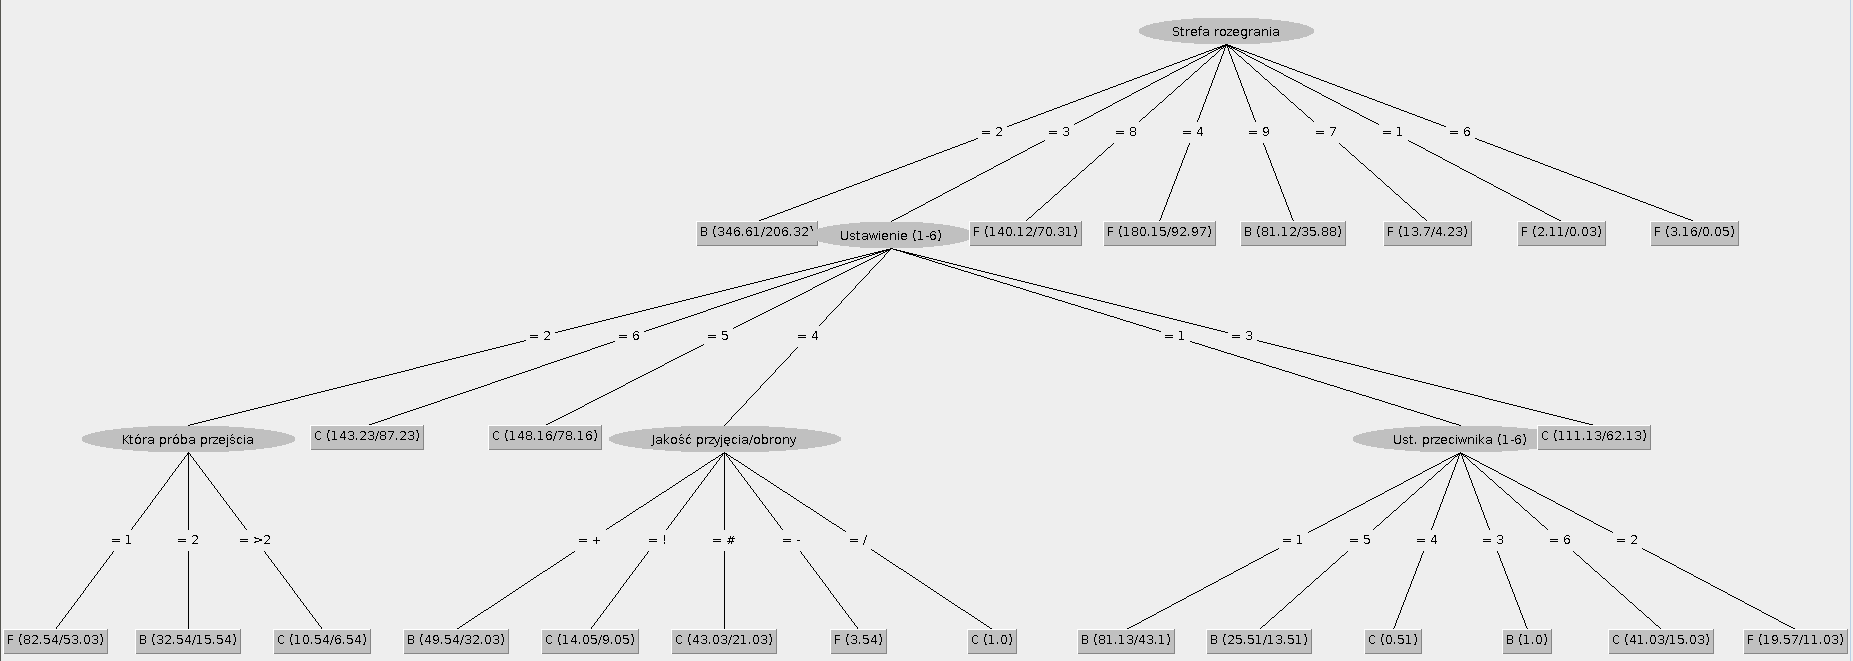
\includegraphics[width=\columnwidth]{drzewoMM2085}
\caption{Drzewo decyzyjne otrzymane jako model klasyfikacyjny przy analizie kierunku rozegrania zawodnika z~największą liczbą wystaw w~bazie danych, dla parametrów minimalnej liczby instancji w~liściach oraz poziomu ufności równych 20 i~0,15.}
\label{fig:drzewo1}
\end{figure}

\begin{figure}
\centering
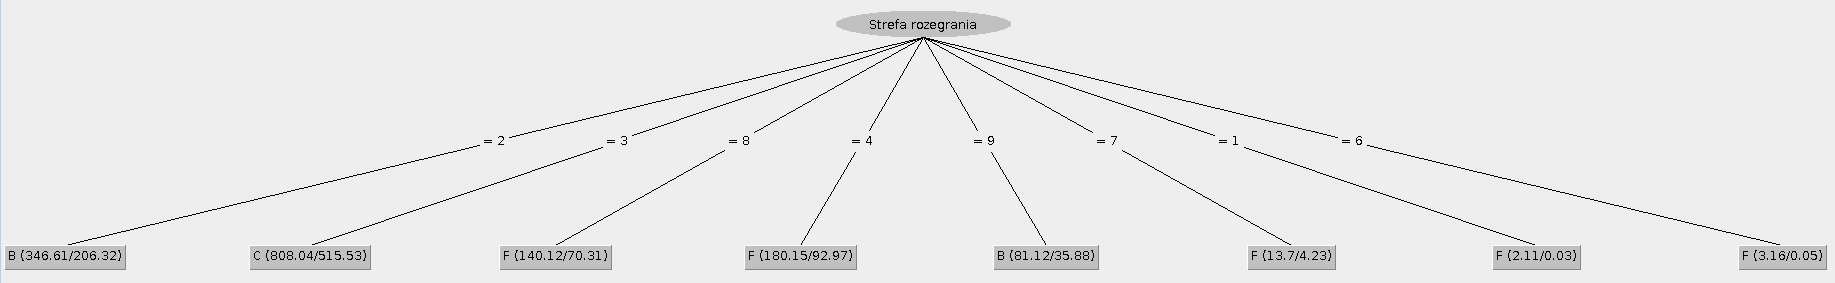
\includegraphics[width=\columnwidth]{drzewoMM2099}
\caption{Drzewo decyzyjne otrzymane jako model klasyfikacyjny przy analizie kierunku rozegrania zawodnika z~największą liczbą wystaw w~bazie danych, dla parametrów minimalnej liczby instancji w~liściach oraz poziomu ufności równych 20 i~0,01.}
\label{fig:drzewo2}
\end{figure}

Oba te drzewa zbudowane zostały do analizy kierunku rozegrania tego samego zawodnika, jednak z~różnymi wartościami parametrów. Dla pierwszego drzewa parametr poziomu ufności jest równy 0,15, natomiast dla drugiego drzewa 0,01. Prełożyło się to na rozmiar obu drzew. Pierwsze znich jest o~rozmiarze 29 (składa się z~24 liści i~5 atrybutów decyzyjnych), a~do podziału wykorystuje 5 różnych atrybutów, natomiast drugie drzewo do podziału wykorzystuje jedynie atrybut o~największej istotności dla tego zawodnika, a~jego rozmiar jest równy 9. Wraz z~uzyskaną wizualizacją drzewa użytkownik otrzymuje również w~konsoli wynik dokładności klasyfikacji oraz wyliczonych miar dla poszczególnych klas (m.in. przedstawionej wcześniej miary $F_1$, precyzji oraz czułości). W~tym przypadku dokładność klasyfikacji dla pierwszego drzewa wyniosła 43,30\%, natomiast dla drugiego drzewa była niższa i~wyniosła 41,84\%.

Na rysunku \ref{fig:drzewo3} przedstawione zostało drzewo dla tego samego zawodnika i~tych samych ustawień parametrów co drzewo z~rysunku \ref{fig:drzewo1}, jednak z~załączoną dodatkowo selekcją atrybutów. Mimo wykorzystanych do budowy tego drzewa tylko czterech wyselekcjonowanych atrybutów drzewo to jest o~wiele większe. Jego rozmiar wynosi 45. Wraz ze wzrostem rozmiaru drzewa stają się mniej czytelne. W~przedstawionej wizualizacji niektóre z~węzłów nachodzą na siebie, jednak w~programie istnieje możliwość przybliżenia danych obszarów drzewa oraz automatycznego skalowania by drzewo było czytelne, jak to zostało przedstawione na rysunku \ref{fig:drzewo4}. Wynik dokładności klasyfikacji dla tego drzewa wyniósł 42,79\%. Na podstawie wyników uzyskanych dla tych trzech drzew widać, że większy rozmiar drzewa nie przykłada się wyższą dokładność.

\begin{figure}
\centering
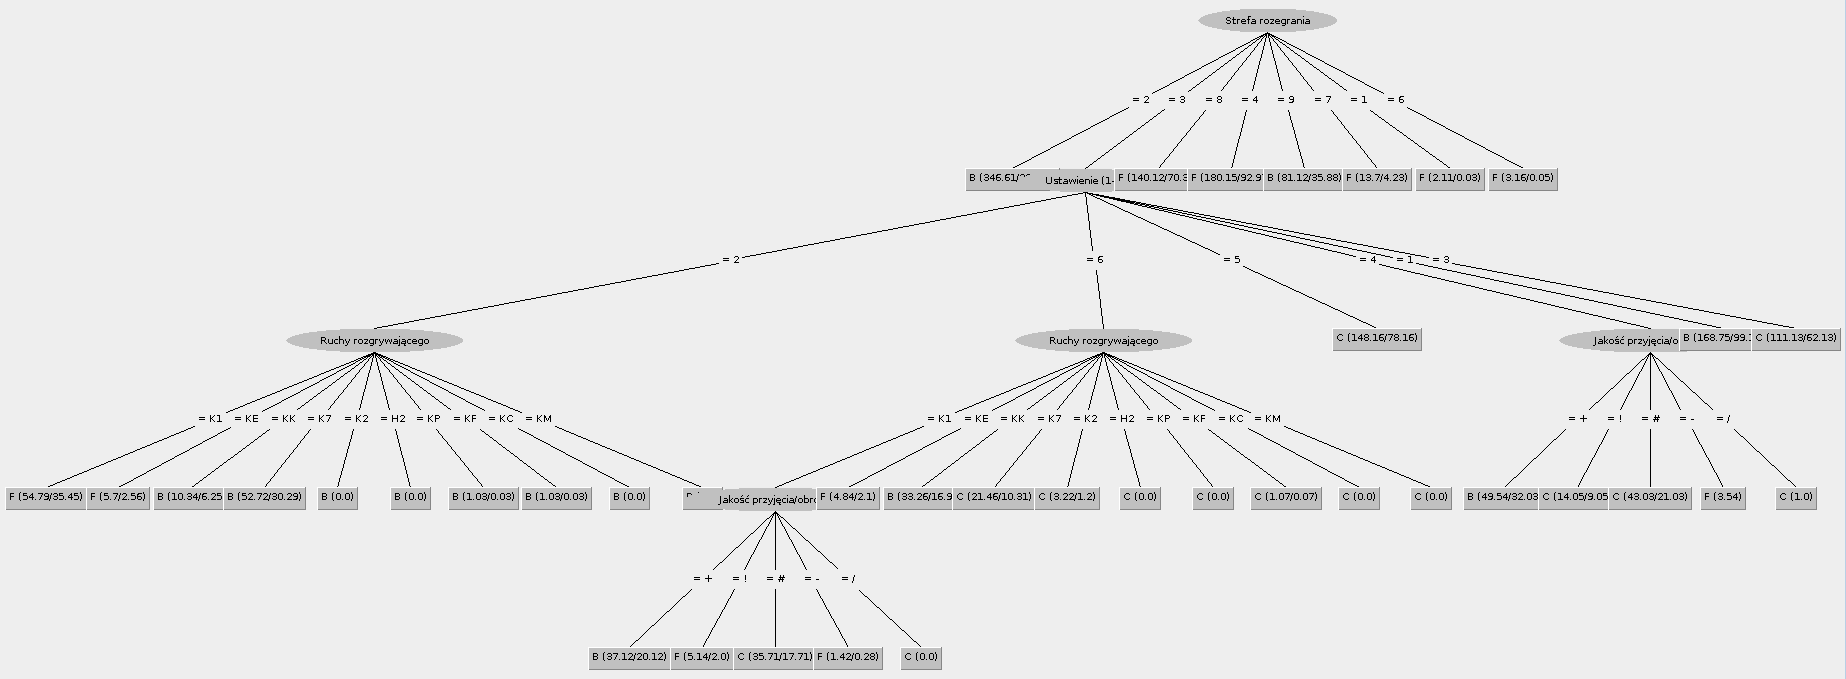
\includegraphics[width=\columnwidth]{drzewoMM2085S}
\caption{Drzewo decyzyjne otrzymane jako model klasyfikacyjny przy analizie kierunku rozegrania zawodnika z~największą liczbą wystaw w~bazie danych, dla parametrów minimalnej liczby instancji w~liściach oraz poziomu ufności równych 20 i~0,15, przy załączonej dodatkowo selekcji atrybutów.}
\label{fig:drzewo3}
\end{figure}

\begin{figure}
\centering
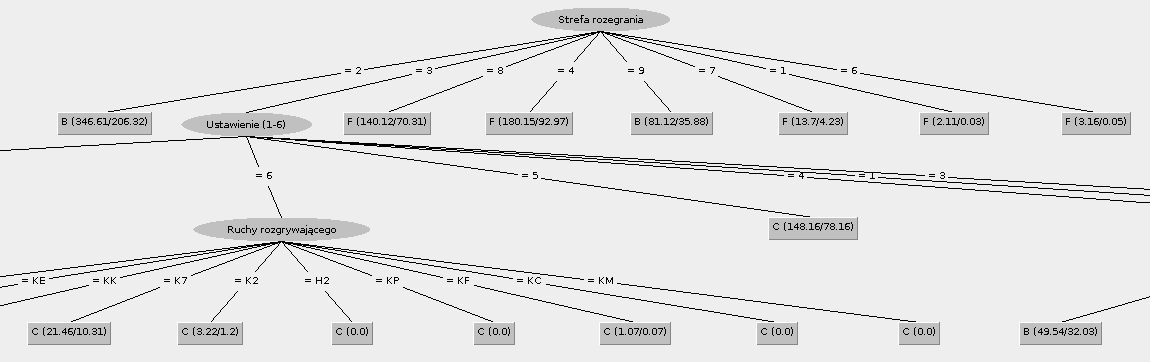
\includegraphics[width=\columnwidth]{drzewoMM2085SP}
\caption{Przybliżony fragment drzewa z~rysunku \ref{fig:drzewo3}.}
\label{fig:drzewo4}
\end{figure}

\subsection{Podział na dane treningowe i~testowe}
\label{roz:podzial-danych}

Wyniki średnich oraz maksymalnych uzyskanych wartości dokładności klasyfikacji dla każdego z~trzech sprawdzonych sposobów podziału na dane treningowe oraz testowe przedstawiono w~tablicach \ref{tab:drzewaKierunekSredniaFolds}, \ref{tab:drzewaKierunekMaxFolds}. Zarówno średnie jak i~maksymalne wartości dokładności klasyfikacji, zmierzone dla drzew decyzyjnych z~10-krotną walidacją krzyżową, są średnio o~ponad 0,2 punktu procentowego większe od wartości uzyskanych dla 5-krotnej walidacji krzyżowej. 

\begin{table}
\centering
\caption{Średnie wartości dokładności klasyfikacji dla drzew decyzyjnych, przy analizie kierunku rozegrania 10 rozgrywających z~największą liczbą wystaw w~bazie danych, w~zależności od sposobu podziału na dane treningowe i~testowe.}
\label{tab:drzewaKierunekSredniaFolds}
\begin{tabular}{rccc}
\toprule
 &            & \multicolumn{2}{c}{$k$-krotna}\\
 & train/test & \multicolumn{2}{c}{walidacja krzyżowa}\\
 \cmidrule{3-4}
inicjały & 80/20 & $k=5$ & $k=10$ \\
\midrule
M.M. & 37,879 & 42,191 & 42,599 \\ 
J.N. & 36,184 & 36,716 & 37,121 \\ 
J.D. & 53,327 & 53,365 & 53,598 \\ 
B.N. & 46,975 & 42,838 & 42,609 \\ 
P.A. & 43,653 & 41,520 & 42,536 \\ 
P.S. & 31,106 & 36,317 & 37,196 \\ 
J.M. & 65,124 & 55,729 & 55,406 \\ 
K.J. & 37,018 & 42,695 & 42,211 \\ 
K.A. & 39,171 & 36,586 & 36,191 \\ 
K.D. & 45,193 & 47,839 & 48,365\\ 
\midrule 
{średnia} & {43,563} & {43,580} & {43,783} \\
\bottomrule
\end{tabular}
\end{table}

\begin{table}
\centering
\caption{Najwyższe wartości dokładności klasyfikacji dla drzew decyzyjnych, przy analizie kierunku rozegrania 10 rozgrywających z~największą liczbą wystaw w~bazie danych, w~zależności od sposobu podziału na dane treningowe i~testowe.}
\label{tab:drzewaKierunekMaxFolds}
\begin{tabular}{rccc}
\toprule
 &            & \multicolumn{2}{c}{$k$-krotna}\\
 & train/test & \multicolumn{2}{c}{walidacja krzyżowa}\\
 \cmidrule{3-4}
inicjały & 80/20 & $k=5$ & $k=10$ \\
\midrule
M.M. & 45,397 & 44,000 & 45,206 \\ 
J.N. & 40,864 & 39,269 & 39,136 \\
J.D. & 56,419 & 55,142 & 55,548 \\
B.N. & 50,741 & 44,428 & 44,354 \\
P.A. & 48,438 & 43,809 & 44,514 \\
P.S. & 39,841 & 39,169 & 40,128 \\
J.M. & 67,811 & 57,560 & 57,646 \\
K.J. & 39,914 & 45,525 & 44,406 \\
K.A. & 42,202 & 38,165 & 37,890 \\
K.D. & 50,495 & 49,205 & 50,000 \\
\midrule 
{średnia} & {48,212} & {45,627} & {45,883} \\
\bottomrule
\end{tabular}
\end{table}

Różnice te są jednak niewielkie w~porównaniu z~wynikami uzyskanymi w~przypadku zwykłego podziału danych w~stosunku 80/20\%. Średnia uzyskana na podstawie wyników wartości średnich wszystkich zawodników jest najniższa, jednak bardzo zbliżona do wartości uzyskiwanych dla walidacji krzyżowej, natomiast średnia wartości maksymalnych jest o~ponad 4 punkty procentowe wyższa. By zbadać istotność tej różnicy przeprowadzony został test statystyczny dla różnicy średnich. Uzyskane wyniki dotyczą tych samych zawodników, w~związku z~czym są to próby zależne, do porównania których (zakładając, że rozkład uzyskanych dokładności klasyfikacji jest normalny) wykorzystać można statystykę testową:
\[t=\frac{\overline{z}}{s_z}\sqrt{n-1}\]

gdzie:
\begin{align*}
	\overline{z} &- \text{średnia różnic między próbami}\\
    s_z &- \text{odchylenie standardowe od uzyskanej średniej różnic}\\
    n &- \text{liczba obserwacji}
\end{align*}
mającą rozkład $t$-Studenta o~$n-1$ stopniach swobody.

Zbadamy hipotezę, że na poziomie istotności $\alpha=0{,}05$ średnia dla maksymalnych wartości uzyskanych za pomocą klasyfikacji z~wykorzystaniem drzew decyzyjnych, przy analizie kierunku rozegrania 10 rozgrywających z~największą liczbą wystaw w~bazie danych, dla podziału danych treningowych i~testowych w~stosunku 80\%/20\% ($\mu_1$) jest równa analogicznej średniej uzyskanej wykorzystując do podziału danych 10-krotną walidację krzyżową ($\mu_2$):
\begin{equation}
H_{0}:\mu_1=\mu_2
\end{equation}
przeciw hipotezie alternatywnej:
\begin{equation}
H_{1}:\mu_1>\mu_2
\end{equation}
\begin{equation}
\overline{z} = \frac{\sum_{i=1}^{n}z_{i}}{n}=2{,}33
\end{equation}
\begin{equation}
s_{z}^{2}=\frac{\sum_{i=1}^{n}(z_{i}-\overline{z})^{2}}{n}=14{,}81
\end{equation}
\begin{equation}
t=\frac{\overline{z}}{s_z}\sqrt{n-1}=1{,}816
\end{equation}
Dla poziomu istotności $\alpha=0{,}05$, $t_{kryt}=t_{0{,}95;9}=1{,}833$ obszar krytyczny to przedział $\langle 1{,}833;+\infty)$. Obliczona statystyka testowa nie należy do obszaru krytycznego zatem nie ma podstaw do odrzucenia hipotezy zerowej. 

Mimo, że test statystyczny nie wykazał istotnej różnicy w~uzyskanych średnich, to analizując wyniki uzyskane w~przypadku klasyfikacji z~podziałem na dane treningowe i~testowe w~stosunku 80/20\% zauważyć można, że różnice dla pojedynczych zawodników, w~stosunku do wyników uzyskiwanych z~wykorzystaną walidacją krzyżową, wahają się od $-5$ punktów procentowych do aż +10 punktów procentowych. Potwierdzeniem tego jest wysoka wartość uzyskana dla sumy wariancji ($s_{z}^{2}=14{,}81$), wyliczonej podczas przeprowadzonego testu statystycznego. To, jaki podzbiór danych będzie uczył, a~jaki testował budowane drzewa decyzyjne, ma więc w~przypadku wykorzystywanych w~tej pracy danych spore znaczenie. Z~tego względu, by ocena dokładności modelu była jak najmniej losowa, w~dalej przeprowadzonych badaniach uzyskane wyniki wykorzystają tylko metodę 10-krotnej walidacji krzyżowej.

\subsection{Wykorzystanie selekcji atrybutów}

\begin{table}
\centering
\caption{Porównanie średnich wartości dokładności klasyfikacji dla drzew decyzyjnych, przy analizie kierunku rozegrania, bez oraz z~włączoną selekcją atrybutów.}
\label{tab:drzewaKierunekSredniaSelekcja}
\begin{tabular}{lrrr}
\toprule
{inicjały} & \multicolumn{1}{c}{\shortstack{\\bez selekcji\\atrybutów}} & \multicolumn{1}{c}{\shortstack{\\z selekcją\\atrybutów}} & \multicolumn{1}{c}{\shortstack{\\liczba\\wyselekcjonowanych\\atrybutów}} \\ 
\midrule
M.M. & 42,599 & 42,646 & 4 \\ 
J.N. & 37,121 & 37,450 & 1 \\ 
J.D. & 53,598 & 54,585 & 3 \\
B.N. & 42,609 & 43,031 & 2 \\ 
P.A. & 42,536 & 42,793 & 3 \\ 
P.S. & 37,196 & 37,951 & 3 \\
J.M. & 55,406 & 56,834 & 4 \\ 
K.J. & 42,211 & 42,089 & 3 \\ 
K.A. & 36,191 & 36,647 & 4 \\
K.D. & 48,365 & 48,469 & 2 \\ 
\midrule
\textbf{średnia} & \textbf{43,783} & \textbf{44,249} & \textbf{2,900} \\ 
\bottomrule
\end{tabular}
\end{table}

\begin{table}
\centering
\caption{Porównanie maksymalnych wartości dokładności klasyfikacji dla drzew decyzyjnych, przy analizie kierunku rozegrania, bez oraz z~włączoną selekcją atrybutów.}
\label{tab:drzewaKierunekMaksSelekcja}
\begin{tabular}{lrrr}
\toprule
{inicjały} & \multicolumn{1}{c}{\shortstack{bez selekcji\\atrybutów}} & \multicolumn{1}{c}{\shortstack{z selekcją\\atrybutów}} & \multicolumn{1}{c}{\shortstack{liczba\\wyselekcjonowanych\\atrybutów}} \\ 
\midrule
M.M. & 45,206 & 44,889 & 4 \\ 
J.N. & 39,136 & 38,007 & 1 \\ 
J.D. & 55,548 & 55,683 & 3 \\
B.N. & 44,354 & 44,799 & 2 \\ 
P.A. & 44,514 & 43,809 & 3 \\ 
P.S. & 40,128 & 40,128 & 3 \\
J.M. & 57,646 & 59,021 & 4 \\ 
K.J. & 44,406 & 44,234 & 3 \\ 
K.A. & 37,890 & 39,266 & 4 \\
K.D. & 50,000 & 49,503 & 2 \\ 
\midrule
\textbf{średnia} & \textbf{45,883} & \textbf{45,934} & \textbf{2,900} \\ 
\bottomrule
\end{tabular}
\end{table}

W tablicach \ref{tab:drzewaKierunekSredniaSelekcja} oraz \ref{tab:drzewaKierunekMaksSelekcja} przedstawiono odpowiednio średnie i~maksymalne wartości dokładności klasyfikacji otrzymane dla drzew decyzyjnych, przy analizie kierunku rozegrania, bez oraz z~włączoną selekcją atrybutów. Co ciekawe zarówno średnia uzyskana z~wyników wszystkich 10 zawodników ich średnich wartości jak i~średnia z~maksymalnych wartości jest wyższa w~przypadku budowy drzew z~wyselekcjonowanymi atrybutami. Jak opisane zostało w~rozdziale \ref{roz:algorytmy} budowa drzew decyzyjnych opiera się na wyborze atrybutów na podstawie wykorzystywanej przy selekcji atrybutów ocenie przyrostu informacji. Wierzchołkiem drzewa jest atrybut o~najwyższym przyroście informacji lub w~przypadku, gdy podane parametry budowy i~przycinania drzewa uniemożliwiły podzielenie danych według tego atrybutu, pojedynczy liść o~wartości najczęściej występującej klasy decyzyjnej. Wybór atrybutów na kolejnych poziomach drzew nie opiera się jednak na rankingu zaprezentowanym w~przypadku wyników selekcji atrybutów, gdyż obliczany przyrost informacji na kolejnych poziomach drzewa dotyczy nie całości danych, a~jedynie danych zaliczających się do badanego poddrzewa. Jak najbardziej może więc wystąpić sytuacja, że atrybut o~niskim przyroście informacji dla całej liczby analizowanych danych może mieć najwyższy przyrost informacji dla danych obejmujących dany węzeł. Wykorzystując selekcję atrybutów, przed zbudowaniem drzewa, niektóre atrybuty, które mogły być wybrane do budowy drzewa zostaną pominięte. W~związku z~tym zmniejsza się często rozmiar drzew (jednak nie zawsze co potwierdzają drzewa z~rysunków \ref{fig:drzewo1} i~\ref{fig:drzewo3}), a~także czas ich budowy, ze względu na mniejszą liczbę atrybutów do sprawdzenia. Jak widać jednak modele drzew decyzyjnych, zbudowane tylko w~oparciu o~tych kilka wyselekcjonowanych atrybutów, mogą dzięki temu, że generalizują większą liczbę przypadków, dawać w~efekcie lepsze wyniki klasyfikacji. Różnice te jednak są niewielkie i~nie dla wszystkich zawodników zastosowanie selekcji atrybutów pozwala uzyskać wyższe wyniki dokładności klasyfikacji.

\begin{figure}
\centering
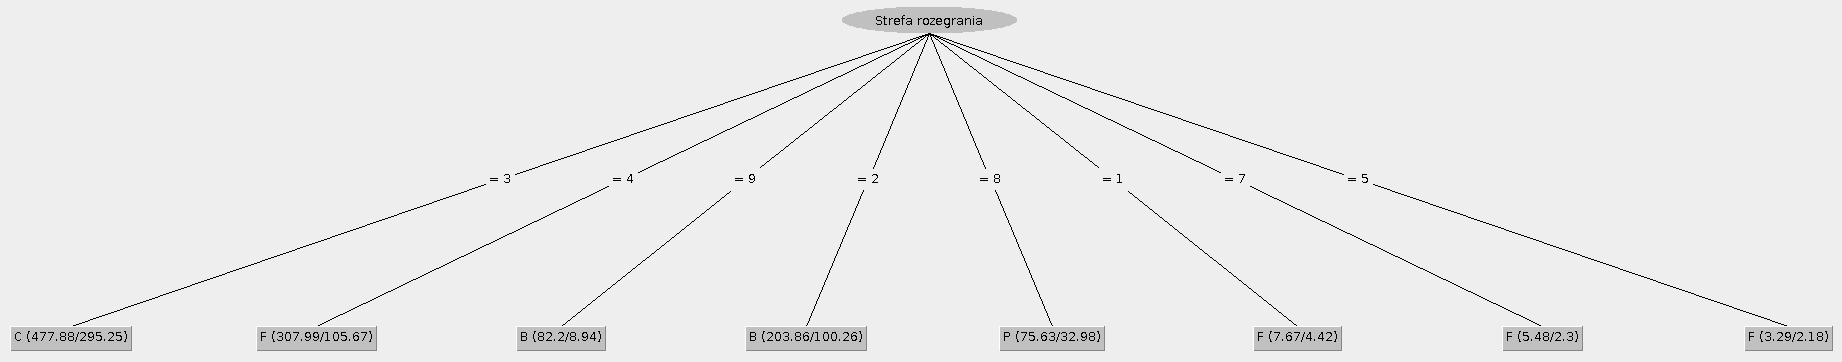
\includegraphics[width=\columnwidth]{drzewoMale}
\caption{Drzewo decyzyjne otrzymane jako model klasyfikacyjny przy analizie kierunku rozegrania zawodnika z~najwyższą średnią dokładnością klasyfikacji, dla parametrów minimalnej liczby instancji w~liściach oraz poziomu ufności równych 25 i~0,01 oraz włączoną selekcją atrybutów.}
\label{fig:drzewo5}
\end{figure}

\begin{figure}
\centering
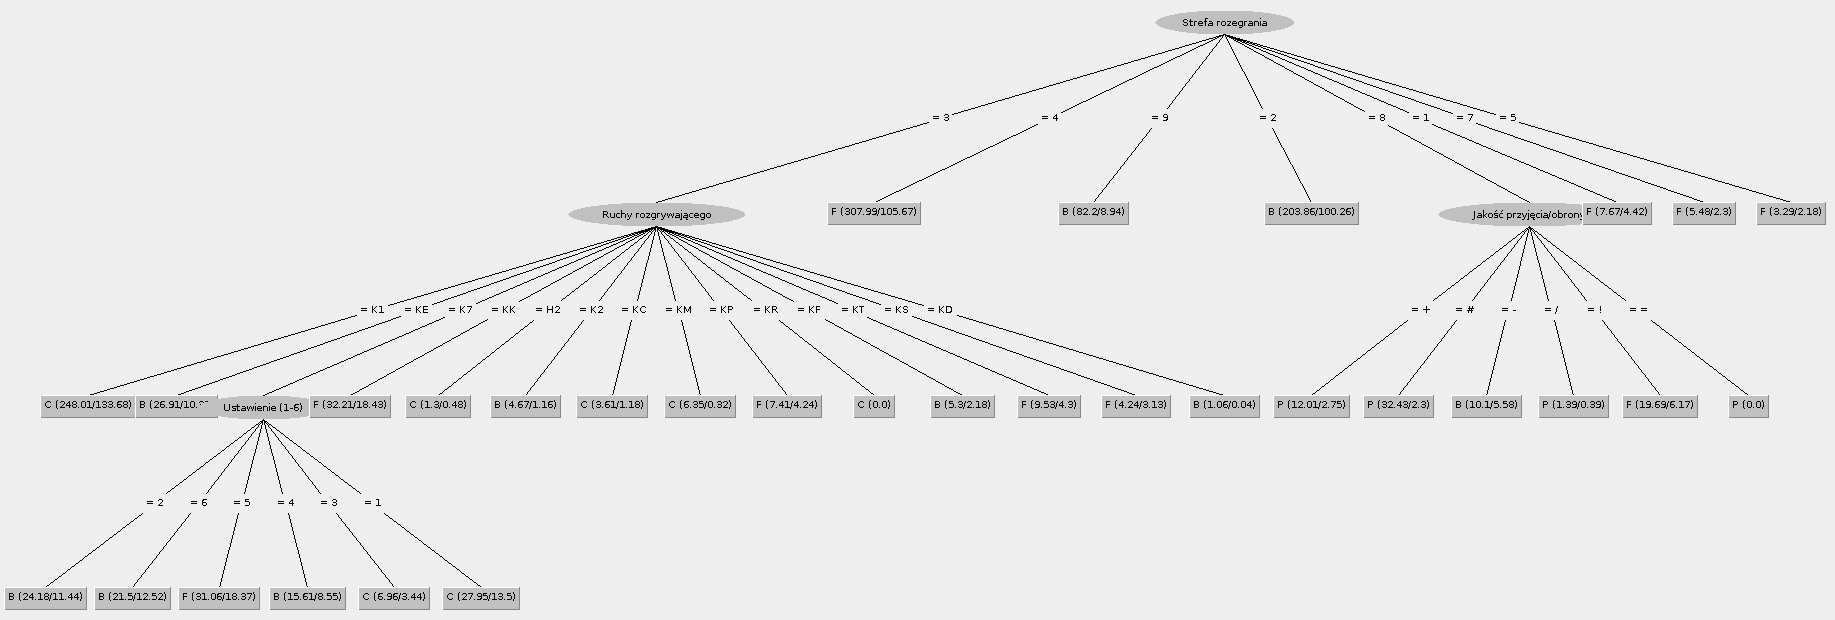
\includegraphics[width=\columnwidth]{drzewoDuze}
\caption{Drzewo decyzyjne otrzymane jako model klasyfikacyjny przy analizie kierunku rozegrania zawodnika z~najwyższą średnią dokładnością klasyfikacji, dla parametrów minimalnej liczby instancji w~liściach oraz poziomu ufności równych 18 i~0,03.}
\label{fig:drzewo6}
\end{figure}

Co ciekawe można znaleźć wiele drzew, otrzymanych dla tych samych zawodników, w~których pomimo znacznych różnic dotyczących rozmiarów drzew wynik dokładności klasyfikacji jest identyczny. Przykładem mogą być drzewa uzyskane dla zawodnika z~najwyższą średnią dokładnością, przedstawione na rysunkach \ref{fig:drzewo5} i~\ref{fig:drzewo6}. W~mniejszym z~drzew wykorzystano zarówno selekcję atrybutów jak i~podano wartości parametrów powodujące obcięcie drzewa tylko do jednego atrybutu. Mimo to oba drzewa osiągnęły dokładność klasyfikacji równą 53,436\%. W~tabeli \ref{tab:drzewaF1} porównane zostały również wyniki miary $F_1$ uzyskane w~przypadku tych drzew dla poszczególnych klas. Obydwa klasyfikatory radzą sobie bardzo podobnie dla najliczniejszych klas: B i~F (dla klasy F uzyskany wynik jest nawet identyczny), natomiast dla mniej licznych klas C i~P występują wyraźne różnice. Mniejsze z~drzew lepiej radzi sobie z~klasyfikacją obserwacji klasy C niż P, a~klasyfikator zbudowany na podstawie większego drzewa radzi sobie z~klasyfikacją tych dwóch klas niemal tak samo -- lepiej niż klasyfikator zbudowany na podstawie mniejszego drzewa z~klasą P, jednak kosztem gorszej klasyfikacji obserwacji należących do klasy C. Klasa P -- wystawy pipe, przez to, że zwykle występują dużo rzadziej, często  nie występują nawet dla mniejszych klasyfikatorów, jak w~przypadku drzewa z~rys.~\ref{fig:drzewo2}. Rozmiar drzew może mieć więc większe znaczenie w~przypadku, gdy chcemy otrzymać klasyfikator, który da jak najlepszy wynik dla najmniej licznych klas.

\begin{table}
\centering
\caption{Porównanie miar $F_1$, wyliczonych dla poszczególnych klas na podstawie drzew decyzyjnych z~rysunku \ref{fig:drzewo5} oraz \ref{fig:drzewo6}.}
\label{tab:drzewaF1}
\begin{tabular}{ccc}
\toprule
{klasa} & \multicolumn{1}{c}{\shortstack{miara $F_1$\\dla drzewa z~rys \ref{fig:drzewo5}}} & \multicolumn{1}{c}{\shortstack{miara $F_1$\\dla drzewa z~rys \ref{fig:drzewo6}}} \\ 
\midrule
B & 0,550 & 0,542 \\ 
F & 0,582 & 0,582 \\ 
C & 0,570 & 0,492 \\
P & 0,408 & 0,497 \\
\bottomrule
\end{tabular}
\end{table}

\subsection{Porównanie z~wartościami oczekiwanymi}

W tabeli \ref{tab:drzewaAOczekiwania} porównane zostały wartości oczekiwane dokładności klasyfikacji z~maksymalnymi wartościami dokładności uzyskanymi metodą klasyfikacji z~wykorzystaniem drzew decyzyjnyh, dla dziesięciu zawodników z~największą liczbą rozegrań zapisanych w~bazie danych, przy analizie kierunku rozegrania. Uzyskane maksymalne wartości polepszają wynik dokładności średnio o~54,73\% w~stosunku do wartości oczekiwanych. Najwyższy wzrost dokładności klasyfikacji w~stosunku do wartości oczekiwanej otrzymany został dla zawodnika o~inicjałach J.M. i~wyniósł aż 104,49\%. Na podstawie wyników w~tabeli nie są widoczne zależności wzrostu dokładności klasyfikacji w~stosunku do wartości oczekiwanej od wyników wartości oczekiwanych. Zawodnik J.M. miał na przykład dopiero piątą w~kolejności najwyższą wartość oczekiwaną wśród zbadanych 10 zawodników. Najniższy wzrost dokładności klasyfikacji, który wyniósł 34,95\%, zaobserwowany został natomiast dla zawodnika B.N., który wartość oczekiwaną miał drugą najwyższą. 

\begin{table}
\centering
\caption{Porównanie wartości oczekiwanych dokładności klasyfikacji z~maksymalnymi wartościami dokładności uzyskanymi metodą klasyfikacji z~wykorzystaniem drzew decyzyjnyh, dla dziesięciu zawodników z~największą liczbą rozegrań zapisanych w~bazie danych, przy analizie kierunku rozegrania.}
\label{tab:drzewaAOczekiwania}
\begin{tabular}{rcccc}
\toprule
inicjały & \multicolumn{1}{c}{\shortstack{wartość\\oczekiwana}} & \multicolumn{1}{c}{\shortstack{maksymalna\\dokładność}} & różnica w~p.p. & \% wzrostu\\ 
\midrule
M.M. & 27,324 & 45,206 & 17,882 & 65,44\\
J.N. & 28,622 & 39,136 & 10,514 & 36,73\\ 
J.D. & 35,672 & 55,683 & 30,011 & 84,13\\
B.N. & 33,196 & 44,799 & 11,603 & 34,95\\ 
P.A. & 28,457 & 44,514 & 16,057 & 56,43\\ 
P.S. & 26,513 & 40,128 & 13,615 & 51,35\\
J.M. & 28,863 & 59,021 & 30,158 & 104,49\\ 
K.J. & 29,163 & 44,406 & 15,243 & 52,27\\ 
K.A. & 28,764 & 39,266 & 10,502 & 36,51\\ 
K.D. & 32,314 & 50,000 & 17,686 & 54,73\\
\midrule
\textbf{średnia} & \textbf{29,889} & \textbf{46,216} & \textbf{17,327} & \textbf{57,70} \\ 
\bottomrule
\end{tabular}
\end{table}

Kluczowym problemem uniemożliwiającym uzyskaniu dzięki klasyfikacji wykorzystywanych w~tych badaniach danych lepszych wyników jest fakt podejmowania przez zawodników decyzji dotyczących analizowanych zagrań w~sposób niedeterministyczny. Mimo występowania nawet dokładnie tych samych wartości atrybutów analizowanych podczas klasyfikacji, jak na przykład dwukrotnej wystawy piłki z~dokładnie tego samego miejsca na boisku, w~tym samym ustawieniu, po przyjęciu tego samego zawodnika i~w tej samej fazie seta w~obu tych zagraniach, przy jednym z~tych zagrań rozgrywający może zdecydować się posłać piłkę na lewe skrzydło, a~za drugim razem na skrzydło prawe. Wynika to z~faktu, że zadaniem rozgrywających jest właśnie gra, ktora będzie jak najmniej przewidywalna dla przeciwnika.


\section{Klasyfikacja kierunku rozegrania z~wykorzystaniem reguł asocjacyjnych}
\label{roz:klasyfikacja-reguly}
Podobnie jak w~przypadku drzew decyzyjnych również w~tym eksperymencie na początku przedstawione zostały przykładowe wyniki, uzyskywane tym razem dzięki metodzie odkrywania reguł asocjacyjnych. Następnie porównane zostały uzyskane wyniki dokładności klasyfikacji bez włączonej selekcji atrybutów oraz z~włączoną selekcją atrybutów. Uzyskane średnie wyniki zostały porównane z~analogicznymi wynikami uzyskanymy metodą klasyfikacji z~wykorzystaniem drzew decyzyjnych. W~przeprowadzonych w~tym eksperymencie badaniach do podziału na dane treningowe oraz testowe wykorzystana została jedynie metoda 10-krotnej walidacji krzyżowej.

\subsection{Wizualizacja odkrywanych reguł asocjacyjnych}
\label{roz:wizReguly}
Wyszukiwane reguły asocjacyjne są wizualizowane użytkownikowi w~postaci listy reguł, spełniających warunki podawanych parametrów, wraz z~rozmiarami uzyskanych zbiorów kandydujących. Przykładem jest lista reguł przedstawiona na rysuku \ref{fig:reguly}. Przy każdej z~reguł podane są informacje o~liczbie instancji spełniających warunki poprzednika oraz wsparciu danej reguły, a~także, będącej wynikiem stosunku tych dwóch liczb, ufności reguły. Lista otrzymanych reguł jest od razu posortowana malejąco według ich ufności, a~przy równej ufności według wsparcia -- również malejąco. 

\begin{figure}
\centering
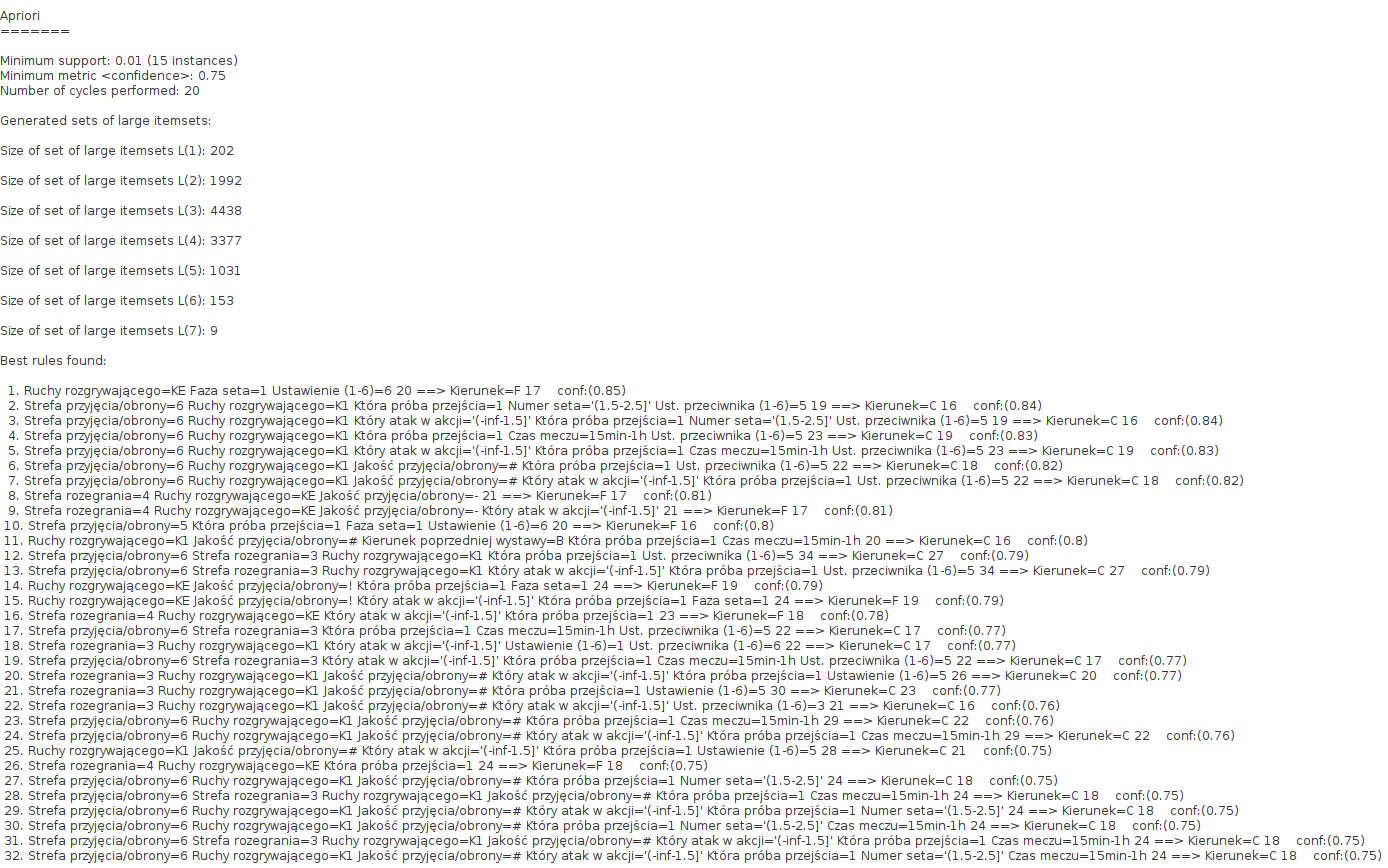
\includegraphics[width=\columnwidth]{reguly}
\caption{Lista reguł otrzymana przy analizie kierunku rozegrania zawodnika z~największą liczbą wystaw w~bazie danych, dla parametrów minimalnej ufności oraz minimalnego wsparcia równych odpowiednio 0,75 i~15.}
\label{fig:reguly}
\end{figure}

Klasyfikacja z~wykorzystaniem reguł opiera się natomiast na modelu zbudowanym z~reguł wyselekcjonowanych w~drugim etapie algorytmu CBA. Na rysunku \ref{fig:reguly-model} przedstawiony został model klasyfikatora zbudowany na podstawie reguł z~rysunku \ref{fig:reguly}. Jak widać w~modelu tym została wykorzystana dokładnie połowa reguł spełniających warunki podanych parametrów. Liczby znajdujące się przy wartościach atrybutów poprzednika reguły określają jedynie numer atrybutu i~numer wartości tego atrybutu przyjęty przez program. Pod listą wyselekcjonowanych reguł znajduje się również informacja o~wybranej końcowej klasie domyślnej dla instancji niepokrytych przez reguły. W~konsoli natomiast, tak samo jak w~przypadku drzew decyzyjnych, wypisane zostają wyniki miar uzyskanych na podstawie klasyfikacji danych testowych.

\begin{figure}
\centering
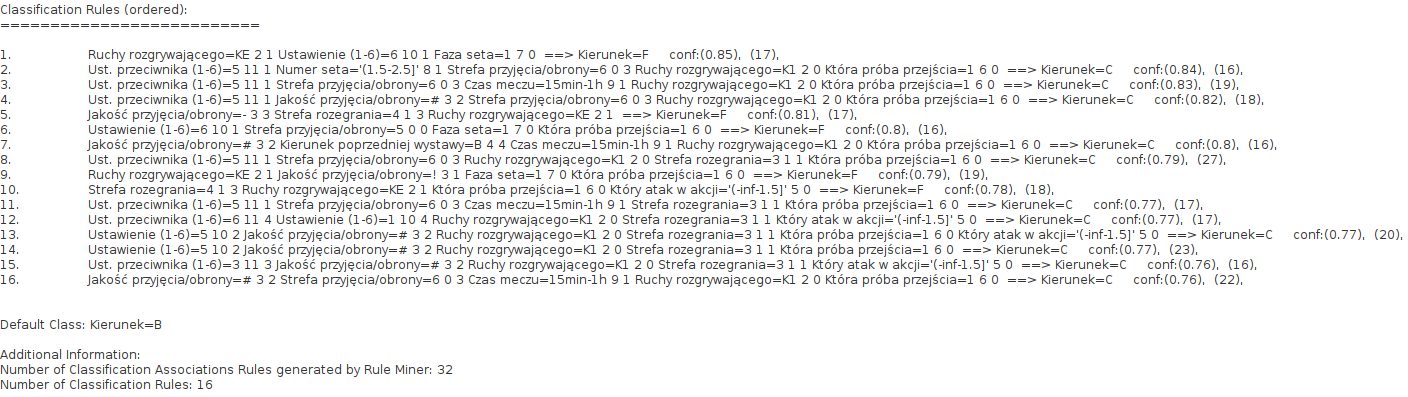
\includegraphics[width=\columnwidth]{reguly-model}
\caption{Model klasyfikacyjny otrzymany na podstawie listy reguł z~rysunku \ref{fig:reguly}}
\label{fig:reguly-model}
\end{figure}

Przy załączonej dodatkowo selekcji atrybutów dla tego samego zawodnika i~tych samych ustawień parametrów otrzymamy jedynie jedną regułę, która występuje również w~liście reguł otrzymanych przy wyłączonej selekcji atrybutów (rys.~\ref{fig:reguly-selekcja}). Wynik dokładności klasyfikacji na podstawie tej pojedynczej reguły oraz klasy domyślnej wyniósł 33,397\%, gdzie dla porównania dokładność klasyfikacji na podstawie reguł otrzymanych bez załączonej selekcji atrybutów wyniósła 36,635\%. 

\begin{figure}
\centering
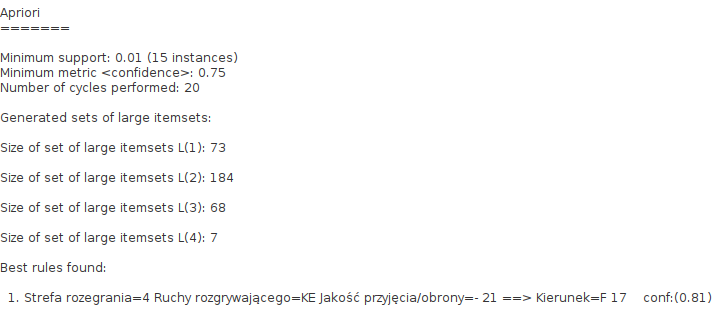
\includegraphics[width=\columnwidth]{reguly-selekcja}
\caption{Lista reguł otrzymana przy analizie kierunku rozegrania zawodnika z~największą liczbą wystaw w~bazie danych, dla parametrów minimalnej ufności oraz minimalnego wsparcia równych odpowiednio 0,75 i~15, z~włączoną selekcją atrybutów.}
\label{fig:reguly-selekcja}
\end{figure}

\subsection{Uzyskane wyniki klasyfikacji}

Ze względu na zwiększenie, w~porównaniu z~metodą drzew decyzyjnych, kroku modyfikacji parametrów, łączny czas badań dla 10 rozgrywających bez selekcji atrybutów został skrócony do 1465,17~sekund, czyli niecałych 25~minut. W~tym czasie zostało przeprowadzonych 30 badań dla każdego z~10 zawodników, więc czas jednego badania wyniósł średnio poniżej 5 sekund. Czas ten jest jednak znacznie dłuższy w~przypadku tworzenia reguł dla niskich wartości parametrów wsparcia i~ufności, niż dla wysokich wartości tych parametrów. Przykładowo dla ustawienia minimalnego wsparcia równego 5 i~minimalnej ufności równej 0,5 czas badania przy analizie kierunku rozegrania zawodnika z~największą liczbą rozegrań wynosi 67,94~sekund. Dla takich ustawień bez ograniczenia do 100 reguł otrzymano by ich aż 35491.

Przy włączonej dodatkowo selekcji atrybutów czas badań dla 10 zawodników zmniejszył się do 175,89~sekund. Zmniejsza się jednak również liczba otrzymywanych reguł. Dla ustawienia wsparcia równego 5 i~ufności równej 0,5, przy analizie kierunku rozegrania zawodnika z~największą liczbą rozegrań, bez ograniczenia do 100 reguł otrzymano już tylko 179 reguł. Ze względu na wykorzystanie selekcji atrybutów, która wskazała 4 atrybuty z~najwyższą wartością oceny, otrzymane 100 reguł z~selekcją atrybutów pokryło blisko 3 razy więcej rekordów niż bez selekcji. Wynika to z~tego, że reguły te posiadały maksymalnie 4 predykaty, w~związku z~czym mogły być bardziej ogólne. Wpływa to zarówno na wynik klasyfikacji, gdyż mniejsza liczba instancji zostanie zaklasyfikowana na podstawie wartości domyślnej zamiast wniosku reguły, a~także na czas badania, ponieważ wyszukiwane zbiory kandydujące mogą być maksymalnie 4 elementowe. Takich w~tym przypadku znaleziono 70, a~bez selekcji atrybutów zbiorów 4-elementowych znaleziono 38027, 5-elementowych 31791 itd. aż do znalezionego jednego zbioru nawet 10-elementowego.

Czasy samego odkrywania reguł asocjacyjnych bez i~z~ograniczeniem do 100 reguł są bardzo podobne. Wynika to z~faktu, że w~algorytmie Apriori wyszukiwane są zbiory częste, a~dopiero później sprawdzana jest ich ufność, na podstawie której reguły te zostają posortowane. Ograniczenie do wykorzystania jedynie 100 reguł asocjacyjnych ma znaczenie natomiast w~samej budowie klasyfikatora na podstawie reguł, gdyż dla każdej kolejnej reguły zgodnie z~algorytmem CBA usuwane są instancje pokryte oraz wyliczana jest dodatkowo liczba błędnie sklasyfikowanych instancji, a~na koniec z~klasyfikatora usuwane są reguły, które nie polepszają uzyskanego wyniki. Samo badanie klasyfikacji bez ograniczenia liczby reguł dla ustawienia wsparcia równego 5 i~ufności równej 0,5, przy analizie kierunku rozegrania zawodnika z~największą liczbą rozegrań trwa ponad 15 minut.

W przypadku zwiększenia wartości parametrów przeszukiwań trzeba mieć jednak na uwadze, że selekcja atrybutów znacznie zmniejsza liczbę znajdowanych reguł. Dla tego samego zawodnika co we wcześniejszych analizach, jednak przy ustawieniu wsparcia równego 15, a~ufności na poziomie 0,7, bez włączonej selekcji atrybutów dostaniemy 69 reguł pokrywających 326 instancji, a~z~włączoną selekcją tylko dwie reguły pokrywające 23 instancje.

\begin{table}
\centering
\caption{Porównanie średnich wartości dokładności klasyfikacji uzyskanych za pomocą klasyfikacji z~użyciem reguł asocjacyjnych, przy analizie kierunku rozegrania, bez włączonej selekcji atrybutów oraz z~nią.}
\label{tab:regulyKierunekSredniaSelekcja}
\begin{tabular}{lrrr}
\toprule
{inicjały} & \multicolumn{1}{c}{\shortstack{bez selekcji\\atrybutów }} & \multicolumn{1}{c}{\shortstack{z selekcją\\atrybutów}} & \multicolumn{1}{c}{\shortstack{liczba\\wyselekcjonowanych\\atrybutów}} \\ 
\midrule
M.M.  & 38,887 & 38,830 & 4\\ 
J.N.  & 34,702 & 34,884 & 1\\ 
J.D.  & 48,866 & 47,323 & 3\\ 
B.N.  & 41,570 & 42,922 & 2\\
P.A.  & 36,212 & 39,472 & 3\\ 
P.S.  & 38,017 & 36,509 & 3\\
J.M.  & 42,892 & 37,706 & 4\\ 
K.J.  & 39,013 & 39,624 & 3\\ 
K.A.  & 36,547 & 38,297 & 4\\ 
K.D.  & 44,652 & 41,952 & 2\\ 
\midrule
\textbf{średnia} & \textbf{40,136} & \textbf{39,752} & \textbf{2,900} \\
\bottomrule
\end{tabular}
\end{table}

\begin{table}
\centering
\caption{Porównanie maksymalnych wartości dokładności klasyfikacji uzyskanych za pomocą klasyfikacji z~użyciem reguł asocjacyjnych, przy analizie kierunku rozegrania, bez włączonej selekcji atrybutów oraz z~nią.}
\label{tab:regulyKierunekMaksSelekcja}
\begin{tabular}{lrrr}
\toprule
{inicjały} & \multicolumn{1}{c}{\shortstack{bez selekcji\\atrybutów }} & \multicolumn{1}{c}{\shortstack{z selekcją\\atrybutów}} & \multicolumn{1}{c}{\shortstack{liczba\\wyselekcjonowanych\\atrybutów}} \\ 
\midrule
M.M.  & 40,063 & 40,508 & 4 \\ 
J.N.  & 36,013 & 34,884 & 1 \\ 
J.D.  & 50,338 & 49,053 & 3 \\ 
B.N.  & 42,125 & 44,725 & 2 \\ 
P.A.  & 37,461 & 44,279 & 3 \\
P.S.  & 39,408 & 37,490 & 3 \\ 
J.M.  & 43,385 & 41,151 & 4 \\ 
K.J.  & 40,964 & 40,361 & 3 \\ 
K.A.  & 38,899 & 39,450 & 4 \\ 
K.D.  & 45,427 & 42,942 & 2 \\ 
\midrule
\textbf{średnia} & \textbf{41,408} & \textbf{41,484} & \textbf{2,900} \\ 
\bottomrule
\end{tabular}
\end{table}

W tablicach \ref{tab:regulyKierunekSredniaSelekcja} i~\ref{tab:regulyKierunekMaksSelekcja} przedstawiono średnie oraz maksymalne wyniki dokładności klasyfikacji uzyskane za pomocą klasyfikacji z~użyciem reguł asocjacyjnych, przy analizie kierunku rozegrania, bez oraz z~włączoną selekcją atrybutów. W~tym przypadku, w~odróżnieniu od klasyfikacji za pomocą drzew decyzyjnych, średnia uzyskana dla średnich wyników bez włączonej selekcji atrybutów jest wyższa, niż z~włączoną selekcją atrybutów. Dla kilku zawodników istnieje jednak spora rozbieżność między maksymalnymi wynikami uzyskanymi przy włączonej oraz wyłączonej selekcji atrybutów. W~przypadku zawodnika o~inicjałach P.A. wartość maksymalna dokładności klasyfikacji uzyskana z~włączoną selekcją atrybutów jest o~blisko 7 punktów procentowych wyższa od maksymalnej dokładności uzyskanej bez selekcji atrybutów. Liczba wyselekcjonowanych atrybutów nie przekłada się na różnice pomiędzy wynikami dokładności klasyfikacji bez selekcji. Przykładowo dla trzech zawodników, dla których wyselekcjonowane zostały aż 4 atrybuty, dwóch z~nich uzyskało wyższe o~około pół punktu procentowego maksymalne wartości dokładności klasyfikacji, natomiast trzeci z~nich uzyskał wartość maksymalną o~ponad 2 punkty procentowe niższą. Podobnie w~przypadku trzech zawodników, dla których wyselekcjonowane zostały mniej niż 3 atrybuty. Dwóch z~nich uzyskało wartości maksymalne niższe przy włączonej selekcji atrybutów o~około 1,5 oraz 2,5 punktu procentowego, natomiast trzeci z~nich przy włączonej selekcji atrybutów uzyskał maksymalną dokładność klasyfikacji o~ponad 2,5 punktu procentowego wyższą niż bez selekcji atrybutów.

\subsection{Porównanie z~wartościami oczekiwanymi oraz wynikami dla drzew decyzyjnych}

W tabeli \ref{tab:regulyAOczekiwania}, podobnie jak dla klasyfikacji z~wykorzystaniem drzew decyzyjnych, porównane zostały maksymalne wartości dokładności uzyskane metodą klasyfikacji z~wykorzystaniem reguł decyzyjnych, dla dziesięciu zawodników z~największą liczbą rozegrań zapisanych w~bazie danych, przy analizie kierunku rozegrania. Uzyskane maksymalne wartoście polepszają w~tym przypadku wynik dokładności średnio o~38,90\% w~stosunku do wartości oczekiwanych. Najwyższy wzrtost dokładności klasyfikacji w~stosunku do wartości oczekiwanej otrzymany został, tak samo jak w~przypadku drzew decyzyjnych, dla zawodnika o~inicjałach J.M. i~wyniósł 50,31\%. Jest to jednak ponad dwukrotnie mniejszy wzrost niż w~przypadku drzew decyzyjnych.

\begin{table}
\centering
\caption{Porównanie wartości oczekiwanych dokładności klasyfikacji z~maksymalnymi wartościami dokładności uzyskanymi metodą klasyfikacji z~wykorzystaniem reguł asocjacyjnych, dla dziesięciu zawodników z~największą liczbą rozegrań zapisanych w~bazie danych, przy analizie kierunku rozegrania.}
\label{tab:regulyAOczekiwania}
\begin{tabular}{rcccc}
\toprule
inicjały & \multicolumn{1}{c}{\shortstack{wartość\\oczekiwana}} & \multicolumn{1}{c}{\shortstack{maksymalna\\dokładność}} & różnica w~p.p. & \% wzrostu\\ 
\midrule
M.M. & 27,324 & 40,508 & 13,184 & 48,25\\
J.N. & 28,622 & 36,013 & 7,391 & 25,82\\ 
J.D. & 35,672 & 50,338 & 14,666 & 41,11\\
B.N. & 33,196 & 42,125 & 8,929 & 26,90\\ 
P.A. & 28,457 & 37,461 & 9,004 & 31,64\\ 
P.S. & 26,513 & 39,408 & 12,895 & 48,64\\
J.M. & 28,863 & 43,385 & 14,522 & 50,31\\ 
K.J. & 29,163 & 40,964 & 11,801 & 40,47\\ 
K.A. & 28,764 & 38,899 & 10,135 & 35,24\\ 
K.D. & 32,314 & 45,427 & 13,113 & 40,58\\
\midrule
\textbf{średnia} & \textbf{29,889} & \textbf{41,453} & \textbf{11,564} & \textbf{38,90} \\
\bottomrule
\end{tabular}
\end{table}

Średnie uzyskane wyniki są niższe od analogicznie uzyskanych dla drzew decyzyjnych (tab.~\ref{tab:drzewaKierunekSredniaSelekcja}, \ref{tab:drzewaKierunekMaksSelekcja}) o~około 4 punkty procentowe. Dla jednego z~zawodników wyniki uzyskane za sprawą klasyfikacji z~użyciem reguł asocjacyjnych są jednak wyższe niż przy użyciu drzew decyzyjnych. W~tabeli \ref{tab:drzewoRegulyF1} porównane zostały natomiast miary $F_1$ uzyskane dla obu metod w~przypadku analizy kierunku rozegrania zawodnika J.M. i~ustawień parametrów analogicznych dla obu tych metod. Na podstawie tej tabeli widać, że klasyfikator wykorzystujący reguły asocjacyjne radzi sobie na podobnym poziomie jedynie z~klasyfikacją klasy $F$, która jest klasą domyślną dla tego klasyfikatora. W~związku z~tym czułość dla tej klasy wyniosła 0,995, jednak prezycja już tylko 0,376. Dla klas $B$ oraz $P$ sytuacja jest natomiast odwrotna: prezycja wyniosła dla nich odpowiednio 0,944 i~1, natomiast czułość jedynie 0,140 i~0,01. Żadna z~instancji nie została natomiast zaklasyfikowana do klasy $C$. Widać więc, że w~przypadku dużej liczby instancji niepokrytych przez reguły, klasyfikacja z~wykorzystaniem reguł asocjacyjnych daje dużo gorsze wyniki dla wszystkich klas poza klasą domyślną.

\begin{table}
\centering
\caption{Porównanie miar $F_1$, wyliczonych dla klasyfikacji z~wykorzystaniem drzew decyzyjnych oraz reguł asocjacyjnych, przy analizie kierunku rozegrania zawodnika J.M., dla parametrów w~przypadku drzew minimalnej liczby instancji i~liściach oraz poziomu ufności równych 18 i~0,03 natomiast w~przypadku reguł asocjacyjnych parametrów minimalnego wsparcia oraz minimalnej ufności równych 18 i~97\%}
\label{tab:drzewoRegulyF1}
\begin{tabular}{ccc}
\toprule
{klasa} & \multicolumn{1}{c}{\shortstack{miara $F_1$ dla\\drzew decyzyjncyh}} & \multicolumn{1}{c}{\shortstack{miara $F_1$ dla\\reguł asocjacyjnych}} \\ 
\midrule
B & 0,542 & 0,245 \\ 
F & 0,582 & 0,546 \\ 
C & 0,492 & - \\
P & 0,497 & 0,020 \\
\bottomrule
\end{tabular}
\end{table}

Na podstawie przedstawionego w~tym rozdziale porównania można stwierdzić, że wykorzystana w~badaniach klasyfikacja z~wykorzystaniem reguł asocjacyjnych daje na ogół gorsze wyniki niż klasyfikacja wykorzystująca drzew decyzyjnych, jednak jest również wartościową metodą klasyfikowania tego typu danych. Zaletą reguł asocjacyjnych, w~przypadku szukania zależności w~grze danego zawodnika, jest natomiast przede wszystkim możliwość skupienia się i~zapamiętania tylko kilku otrzymanych reguł posiadających najwyższe wartości wsparcia oraz ufności, które mogą pozwolić przewidzieć sporą liczbę zagrań.

\section{Zależność wyników klasyfikacji od wartości parametrów przeszukiwań}
\label{roz:eks-parametry}

W tym eksperymencie przeanalizowane zostały zależności uzyskiwanych wyników dokładności klasyfikacji od wartości parametrów używanych przy budowie drzew decyzyjnych oraz wyszukiwania reguł asocjacyjnych. W~tym celu ponownie wykorzystano wyniki klasyfikacji kierunku rozegrania uzyskane dla rozgrywających z~największą liczbą rozegrań. Do analizy zależności uzyskiwanych wyników od parametrów używanych przy budowie drzew wykorystano wyniki uzyskane dla 10 zawodników z~największą liczbą rozegrań w~bazie danych, natomiast w~przypadku zależności od parametrów używanych przy wyszukiwaniu reguł asocjacyjnych, ze względu na czas wykonywanych badań, wykorzystane zostały wyniki uzyskane tylko dla dwóch zawodników. Celem tych badań była próba znalezienia optymalnych wartości parametrów, czyli takich dla których uzyskiwane wyniki dokładności klasyfikacji będą najwyższe. 

\subsection{Drzewa decyzyjne}
\subsubsection{Parametr minimalnej liczby instancji}

Na rysunku \ref{fig:support-r-kierunek} przedstawiającym wyniki zależności średniej wartości dokładności klasyfikacji od parametru minimalnej liczby instancji, przy analizie kierunku rozegrania, zauważyć można, że najwyższa średnia wartość dokładności osiągana jest dla parametru równego 15, a~najmniejsza dla najmniejszych badanych wartości parametru, czyli od 2 do 4. Analizując ten wykres można by stwierdzić, że w~ten sposób znaleziono wartość minimalnej liczby instancji, dla której przy analizie kierunku rozegrania metodą drzew decyzyjnych otrzymywane wartości accuracy są najwyższe. Gdy jednak przyjrzymy się wynikom dla dwójki rozgrywających o~najwyższej (rys.~ \ref{fig:support-r-kierunek-best}) i~najniższej (rys.~\ref{fig:support-r-kierunek-worst}) średniej wartości accuracy z~dziesiątki badanych, że dla każdego z~nich rozkład wyników zależnych od wartości supportu jest zupełnie inny. Uśredniony wynik dla wszystkich dziesięciu zawodników pozwala natomiast wskazać zakres wartości supportu, w~którym warto rozpocząć przeszukiwania, tak by otrzymać drzewo decyzyjne o~najwyższej wartości accuracy. Dla każdego zawodnika optymalny dobór tego parametru może być jednak inny. 

\begin{figure}
\centering
\begin{tikzpicture}
\begin{axis}[
    y tick label style={xlabel=min. liczba instancji, ylabel=dokładność, y unit=\%, 
        /pgf/number format/.cd, use comma, 
            fixed,   % po zakomentowaniu os rzednych jest indeksowana wykladniczo
            fixed zerofill, % 1.0 zamiast 1
            precision=1,
        /tikz/.cd
    },
    x tick label style={
        /pgf/number format/.cd, use comma, 
            fixed,
            %fixed zerofill,
            %precision=2,
        /tikz/.cd
    }
]
\addplot table [x=support, y=srednia, col sep=semicolon, /pgf/number format/read comma as period, ignore chars={"}] {wyniki/support-rozegranie-kierunki.csv};
\end{axis}
\end{tikzpicture}
\caption{Wykres zależności średniej wartości dokładności klasyfikacji od wartości parametru minimalnej liczby instancji, dla dziesięciu rozgrywających z~największą liczbą wystaw, przy analizie kierunku rozegrania za pomocą drzew decyzyjnych.}
\label{fig:support-r-kierunek}
\end{figure}

\begin{figure}
\centering
\begin{tikzpicture}
\begin{axis}[xlabel=min. liczba instancji, ylabel=dokładność, y unit=\%, 
    y tick label style={
        /pgf/number format/.cd,
            fixed,   % po zakomentowaniu os rzednych jest indeksowana wykladniczo
            fixed zerofill, % 1.0 zamiast 1
            precision=1,
        /tikz/.cd
    }
]
\addplot table [x=support, y=best, col sep=semicolon, /pgf/number format/read comma as period, ignore chars={"}] {wyniki/support-rozegranie-kierunki.csv};
\end{axis}
\end{tikzpicture}
\caption{Wykres zależności średniej wartości dokładności klasyfikacji od wartości parametru minimalnej liczby instancji, dla rozgrywającego z~najwyższą średnią wartością dokładności, przy analizie kierunku rozegrania za pomocą drzew decyzyjnych.}
\label{fig:support-r-kierunek-best}
\end{figure}

\begin{figure}
\centering
\begin{tikzpicture}
\begin{axis}[xlabel=min. liczba instancji, ylabel=dokładność, y unit=\%, 
    y tick label style={
        /pgf/number format/.cd, 
        	use comma, 
            fixed,   % po zakomentowaniu os rzednych jest indeksowana wykladniczo
            fixed zerofill, % 1.0 zamiast 1
            precision=1,
        /tikz/.cd
    }
]
\addplot table [x=support, y=worst, col sep=semicolon, /pgf/number format/read comma as period, ignore chars={"}] {wyniki/support-rozegranie-kierunki.csv};
\end{axis}
\end{tikzpicture}
\caption{Wykres zależności średniej wartości dokładności klasyfikacji od wartości parametru minimalnej liczby instancji, dla rozgrywającego z~najniższą średnią wartością dokładności, przy analizie kierunku rozegrania za pomocą drzew decyzyjnych.}
\label{fig:support-r-kierunek-worst}
\end{figure}

Omówione zależności są widoczne na przedstawionych wykresach tylko ze wzglę\-du na to, że zakres wartości na osi y został ograniczony do najmniejszej i~największej uzyskanej wartości, a~nie całego przedziału możliwych wartości, czyli od 0 do 100. Wykres dla tej samej serii danych co w~przypadku rysunku \ref{fig:support-r-kierunek} jednak z~pełnym zakresem możliwych wartości na osi $y$ został przedstawiony na rysunku \ref{fig:support-r-kierunek100}. Na tym wykresie uzyskane wyniki dla poszczególnych wartości parametrów wydają się identyczne. W~związku z~tym przeprowadzony został również test statystyczny sprawdzający, podobnie jak w~przypadku eksperymentu z~podziałem na dane treningowe i~testowe (rozdział \ref{roz:podzial-danych}), istotność różnic dwóch średnich. W~tabeli \ref{tab:support-r-kierunek} przedstawiono średnie wartości dokładności klasyfikacji uzyskane dla dziesięciu rozgrywających z~największą liczbą wystaw, przy analizie kierunku rozegrania za pomocą drzew decyzyjnych, dla ustawień parametrów minimalnej liczby instancji równych 2 i~15.

\begin{figure}
\centering
\begin{tikzpicture}
\begin{axis}[
    y tick label style={xlabel=min. liczba instancji, ylabel=dokładność, y unit=\%, 
        /pgf/number format/.cd, use comma,
        ymin=0, 
        ymax=100,
            fixed,   % po zakomentowaniu os rzednych jest indeksowana wykladniczo
            fixed zerofill, % 1.0 zamiast 1
            precision=1,
        /tikz/.cd
    },
    x tick label style={
        /pgf/number format/.cd, use comma, 
            fixed,
            %fixed zerofill,
            %precision=2,
        /tikz/.cd
    }
]
\addplot table [x=support, y=srednia, col sep=semicolon, /pgf/number format/read comma as period, ignore chars={"}] {wyniki/support-rozegranie-kierunki.csv};
\end{axis}
\end{tikzpicture}
\caption{Wykres przedstawiony na rysunku \ref{fig:support-r-kierunek} dla pełnego przedziału możliwych wartości na osi y}
\label{fig:support-r-kierunek100}
\end{figure}

\begin{table}
\centering
\caption{Porównanie średnich wartości dokładności klasyfikacji uzyskanych dla dziesięciu rozgrywających z~największą liczbą wystaw, przy analizie kierunku rozegrania za pomocą drzew decyzyjnych, dla ustawień parametrów minimalnej liczby instancji równych 2 i~15.}
\label{tab:support-r-kierunek}
\begin{tabular}{lcc}
\toprule
{inicjały} & \multicolumn{1}{c}{\shortstack{średnia dokładność dla\\parametru równego 2}} & \multicolumn{1}{c}{\shortstack{średnia dokładność dla\\parametru równego 15}}\\ 
\midrule
M.M.  & 40,927 & 42,499 \\ 
J.N.  & 35,948 & 37,268 \\ 
J.D.  & 52,268 & 53,873 \\ 
B.N.  & 41,887 & 42,359 \\ 
P.A.  & 40,071 & 43,158 \\
P.S.  & 36,368 & 38,681 \\ 
J.M.  & 54,778 & 55,833 \\ 
K.J.  & 41,339 & 42,184 \\ 
K.A.  & 35,240 & 36,444 \\ 
K.D.  & 48,058 & 49,036 \\ 
\midrule
\textbf{średnia} & \textbf{42,688} & \textbf{44,134} \\ 
\bottomrule
\end{tabular}
\end{table} 

Na podstawie danych z~tej tableli zbadana zostanie hipoteza, że na poziomie istotności $\alpha = 0,05$ średnia dokładność klasyfikacji dla uzyskana dla wartości parametru minimalnej liczby instancji równej 15 ($\mu_1$), jest równa analogicznej średniej uzyskanej dla wartości parametru minimalnej liczby instancji równej 2 ($\mu_2$):
\begin{equation}
H_{0}:\mu_1=\mu_2
\end{equation}
przeciw hipotezie alternatywnej:
\begin{equation}
H_{1}:\mu_1>\mu_2
\end{equation}
\begin{equation}
\overline{z} = \frac{\sum_{i=1}^{n}z_{i}}{n}=1,445
\end{equation}
\begin{equation}
s_{z}^{2}=\frac{\sum_{i=1}^{n}(z_{i}-\overline{z})^{2}}{n}=0,724
\end{equation}
\begin{equation}
t=\frac{\overline{z}}{s_z}\sqrt{n-1}=5,988
\end{equation}
Dla poziomu istotności $\alpha=0,05$, $t_{kryt}=t_{0,95;9}=1,833$ obszar krytyczny to przedział $\langle 1,833;+\infty)$. Obliczona statystyka testowa należy do obszaru krytycznego zatem odrzucamy hipotezę zerową i~przyjmujemy hipotezę alternatywną. Na podstawie tego testu widać więc, że uzyskane średnie różnią się istotnie od siebie. Dodatkowo, w~przypadku problemu poruszanego w~badaniach, każdy drobny wzrost dokładności klasyfikacji może przełożyć się na końcowy wynik rozgrywanych meczów. Różnica uzyskanych średnich wynosi około 1,5 punktu procentowego, w~związku z~czym w~przypadku 200 rozegrań, których liczba może być nawet większa w~przypadku pięciosetowych pojedynków, około 3 rozegrania więcej zostaną poprawnie przewidziane. W~przypadku bardzo wyrównanego spotkania poprawne przewidzenie nawet pojedynczego zagrania więcej, może okazać się kluczowe do zdobycia punktu na wagę zwycięstwa w~meczu.

\begin{figure}
\centering
\begin{tikzpicture}
\begin{axis}[xlabel=min. liczba instancji, ylabel=dokładność, y unit=\%, 
    y tick label style={
        /pgf/number format/.cd, 
        	use comma, 
            fixed,   % po zakomentowaniu os rzednych jest indeksowana wykladniczo
            fixed zerofill, % 1.0 zamiast 1
            precision=1,
        /tikz/.cd
    }
]
\addplot table [x=support, y=auto, col sep=semicolon, /pgf/number format/read comma as period, ignore chars={"}] {wyniki/support-rozegranie-kierunki.csv};
\end{axis}
\end{tikzpicture}
\caption{Wykres zależności średniej wartości dokładności klasyfikacji od wartości parametru minimalnej liczby instancji, dla dziesięciu rozgrywających z~największą liczbą wystaw, przy analizie kierunku rozegrania za pomocą drzew decyzyjnych, z~włączoną selekcją atrybutów.}
\label{fig:support-r-kierunek-auto}
\end{figure}

Na rysunku \ref{fig:support-r-kierunek-auto} przedstawiono również zależność średniej wartości dokładności klasyfikacji od parametru minimalnej liczby instancji przy analizie kierunku rozegrania, jednak dodatkowo z~włączoną selekcją atrybutów. W~tym przypadku widać, że wyniki uzyskiwane dla wartości parametru mniejszej niż 15, są wyższe niż dla parametru większego niż 15. Włączenie selekcji atrybutów powoduje już znaczne ograniczenie rozbudowania drzewa, przez co dla wyższych wartości minimalnej liczby instancji, powodujących dodatkowe przycinanie drzewa otrzymane wyniki są przez to zauważalnie niższe. Przedział od najniższej do najwyższej średniej wartości dokładności uzyskanej przy włączonej selekcji atrybutów wynosi już jednak tylko nieco ponad pół punktu procentowego.

\subsubsection{Parametr poziomu ufności -- przycinanie drzewa}

Podobnie jak w~przypadku parametru minimalnej liczby instancji również dobór odpowiedniej wartości parametru poziomu ufności jest sprawą indywidualną dla każdego z~zawodników. Na rysunku \ref{fig:confidence-r-kierunek}, prezentującym zależności średniej wartości dokładności klasyfikacji od wartości parametru poziomu ufności, dla dziesięciu rozgrywających z~największą liczbą wystaw, przy analizie kierunku rozegrania, można zauważyć jednak pewne zależności. Wraz ze wzrostem początkowych badanych wartości parametru od 0.01 do 0.1, średnia wartość dokładności znacząco rośnie. Czym mniejsza wartość poziomu ufności tym mocniejsze przycinanie drzewa, przez co w~tym przedziale wynikiem drzewa jest zwykle pojedynczy liść lub rozbicie na tylko jeden z~atrybutów. Najwyższe wartości uzyskiwane są w~przedziale od 0,1 do 0,25, w~którym to stosunek źle sklasyfikowanych obserwacji z~próby testowej do wszystkich obserwacji jest niewielki, jednak przycinanie w~tym przedziale nie jest na tyle silne, by uniemożliwić rozbicie drzew na kilka atrybutów. Dla wyższych wartości poziomu ufności niż 0,25 średnia wartość dokładności maleje za to praktycznie jednostajnie. Świadczy to o~pozytywnym działaniu przycinania drzewa, które będąc zbyt słabe w~wyniku daje drzewa o~niższej dokładności klasyfikacji, a~dodatkowo silnie rozbudowane i~ciężkie do analizy.

\begin{figure}
\centering
\begin{tikzpicture}
\begin{axis}[xlabel=poziom ufności, ylabel=dokładność, y unit=\%, 
    y tick label style={
        /pgf/number format/.cd,
        	use comma,
            fixed,
            fixed zerofill, 
            precision=1,
        /tikz/.cd
    },
    x tick label style={
        /pgf/number format/.cd,
        	use comma,
            fixed,
            fixed zerofill,
            precision=2,
        /tikz/.cd
    }
]
\addplot table [x=confidence, y=srednia, col sep=semicolon, /pgf/number format/read comma as period, ignore chars={"}] {wyniki/confidence-rozegranie-kierunki.csv};
\end{axis}
\end{tikzpicture}
\caption{Wykres zależności średniej wartości dokładności klasyfikacji od wartości poziomu ufności, dla dziesięciu rozgrywających z~największą liczbą wystaw, przy analizie kierunku rozegrania za pomocą drzew decyzyjnych.}
\label{fig:confidence-r-kierunek}
\end{figure}

\begin{figure}
\centering
\begin{tikzpicture}
\begin{axis}[xlabel=poziom ufności, ylabel=dokładność, y unit=\%, 
    y tick label style={
        /pgf/number format/.cd,
        	use comma,
            fixed,
            fixed zerofill,
            precision=1,
        /tikz/.cd
    },
    x tick label style={
        /pgf/number format/.cd,
        	use comma,
            fixed,
            fixed zerofill,
            precision=2,
        /tikz/.cd
    }
]
\addplot table [x=confidence, y=best, col sep=semicolon, /pgf/number format/read comma as period, ignore chars={"}] {wyniki/confidence-rozegranie-kierunki.csv};
\end{axis}
\end{tikzpicture}
\caption{Wykres zależności średniej wartości dokładności klasyfikacji od wartości poziomu ufności, dla rozgrywającego z~najwyższą średnią wartością accuracy, przy analizie kierunku rozegrania za pomocą drzew decyzyjnych.}
\label{fig:confidence-r-kierunek-best}
\end{figure}

\begin{figure}
\centering
\begin{tikzpicture}
\begin{axis}[xlabel=poziom ufności, ylabel=dokładność, y unit=\%, 
    y tick label style={
        /pgf/number format/.cd,
        	use comma,
            fixed,
            fixed zerofill,
            precision=1,
        /tikz/.cd
    },
    x tick label style={
        /pgf/number format/.cd,
        	use comma,
            fixed,
            fixed zerofill,
            precision=2,
        /tikz/.cd
    }
]
\addplot table [x=confidence, y=worst, col sep=semicolon, /pgf/number format/read comma as period, ignore chars={"}] {wyniki/confidence-rozegranie-kierunki.csv};
\end{axis}
\end{tikzpicture}
\caption{Wykres zależności średniej wartości dokładności klasyfikacji od wartości poziomu ufności, dla rozgrywającego z~najniższą średnią wartością accuracy, przy analizie kierunku rozegrania za pomocą drzew decyzyjnych.}
\label{fig:confidence-r-kierunek-worst}
\end{figure}

Przy analizie parametru poziomu ufności dla zawodnika o~najwyższej średniej wartości dokładności klasyfikacji (rys.~\ref{fig:confidence-r-kierunek-best}) widać podobne zależności, jak w~przypadku średniej uzyskanej na podstawie wyników dziesięciu rozgrywających, jednak w~tym przypadku zauważalne są wyższe o~około pół punktu procentowego wartości dokładności w~przedziale confidence od 0,41 do 0,5 w~stosunku do przedziału od 0,33 do 0,4. Słabsze przycięcie drzewa miało w~tym przypadku więc pozytywny efekt na wyniku dokładności, w~związku z~czym nie można więc stwierdzić, że wartość dokładności klasyfikacji rzeczywiście maleje wraz ze wzrostem tego parametru w~przedziale od 0,25 do 0,5. 

Dla zawodnika o~najniższej średniej wartości dokładności klasyfikacji najwyższe wartości uzyskiwane są za to dla wartości poziomu ufności równych od 0,01 do 0,08 (rys.~\ref{fig:confidence-r-kierunek-worst}). W~przypadku tego zawodnika najwyższy wynik równy 37,890 uzyskano dla parametru minimalnej liczby instancji równego 15 i~parametru poziomu ufności równemu 0.33 oraz 0.34. Otrzymane wówczas drzewo składa się z~15 węzłów. Nieco tylko niższy wynik, równy 37,798, uzyskany został natomiast w~przypadku na tyle silnego przycięcia drzewa, że jego wynikiem był pojedynczy węzeł. Wynik w~postaci jednego węzła, dla dowolnej wartości minimalnej liczby instancji, otrzymany został właśnie w~przedziale confidence od 0,01 do 0,08, przez co średnia wartość dokładności klasyfikacji w~tym przedziale jest najwyższa. Może więc wystąpić również sytuacja, w~której podział na którykolwiek z~analizowanych atrybutów okaże się gorszy, niż samo zaobserwowanie najczęściej występującej klasy decyzyjnej. 

\begin{figure}
\centering
\begin{tikzpicture}
\begin{axis}[xlabel=poziom ufności, ylabel=dokładność, y unit=\%, 
    y tick label style={
        /pgf/number format/.cd,
        	use comma,
            fixed,
            fixed zerofill,
            precision=1,
        /tikz/.cd
    },
    x tick label style={
        /pgf/number format/.cd,
        	use comma,
            fixed,
            fixed zerofill,
            precision=2,
        /tikz/.cd
    }
]
\addplot table [x=confidence, y=auto, col sep=semicolon, /pgf/number format/read comma as period, ignore chars={"}] {wyniki/confidence-rozegranie-kierunki.csv};
\end{axis}
\end{tikzpicture}
\caption{Wykres zależności średniej wartości dokładności klasyfikacji od wartości poziomu ufności, dla dziesięciu rozgrywających z~największą liczbą wystaw, przy analizie kierunku rozegrania za pomocą drzew decyzyjnych, z~włączoną selekcją atrybutów.}
\label{fig:confidence-r-kierunek-auto}
\end{figure}

Gdy dodatkowo załączona zostaje selekcja atrybutów średnia wartość dokładności rośnie znacząco wraz ze wzrostem wartości poziomu ufności od 0,01 do 0,2 (rys.~\ref{fig:confidence-r-kierunek-auto}). Wynika to z~podwójnego ograniczenia rozbudowania drzewa - zarówno poprzez selekcję atrybutów jak i~późniejsze przycinanie drzewa. Dla wartości poziomu ufności wyższej od 0,2 średnia wartość dokładności jest bardzo zbliżona do siebie, jednak najwyższa gdy przycięcie jest najsłabsze czyli dla wartości tego parametru w~przedziale od 0,48 do 0,5.

\subsection{Reguły asocjacyjne}

Jak zostalo opisane w~rozdziale \ref{roz:metodyka} w~przypadku klasyfikacji z~użyciem reguł asocjacyjnych, przeprowadzenie badań z~taką samą modyfikacją parametrów jak w~przypadku drzew decyzyjnych dla dwóch zawodników trwało ponad 12 godzin. Dla dziesięciu zawodników, testowanych w~przypadku drzew decyzynych, czas ten wyniósłby więc około 60 godziny, czyli 2 i~pół dnia. Otrzymane wyniki dla dwóch zawodników pozwalają jednak zauważyć pewne zależności

\subsubsection{Parametr minimalnego wsparcia reguł}

W przypadku wykresu zależności średniej wartości dokładności klasyfikacji od wartości parametru minimalnego wsparcia reguł (tab.~\ref{fig:support-r-kierunek-rules}) widać, że dla początkowych wartości parametru (2-5) średnia wartość dokładności jest stała. W~tym przedziale bowiem wszystkie otrzymywane 100 reguł ma pewność równą 100\%. Dla kolejnych wartości parametru minimalnego wsparcia średnia wartość dokładności dla tych dwóch zawodników nieco maleje, osiągając najniższą średnią dla parametru równego 8. Dla kolejnych wartości parametrów zauważalny jest wzrost średniej dokładności, jednak nie jest on jednostajny. Wyniki działania dla tej metody zależą bowiem przede wszystkim od liczby pokrytych instancji. Wraz ze wzrostem minimalnego wsparcia, otrzymywane reguły mają zwykle coraz niższą pewność, jednak pokrywa większą liczbę instancji, dzięki czemu mniejsza liczba instancji zostaje zaklasyfikowana na podstawie wartości domyślnej.

\begin{figure}
\centering
\begin{tikzpicture}
\begin{axis}[
    y tick label style={xlabel=min. wsparcie, ylabel=dokładność, y unit=\%, 
        /pgf/number format/.cd,
        	use comma,
            fixed,   % po zakomentowaniu os rzednych jest indeksowana wykladniczo
            fixed zerofill, % 1.0 zamiast 1
            precision=1,
        /tikz/.cd
    },
    x tick label style={
        /pgf/number format/.cd,
        	use comma,
            fixed,
            %fixed zerofill,
            %precision=2,
        /tikz/.cd
    }
]
\addplot table [x=support, y=rules, col sep=semicolon, /pgf/number format/read comma as period, ignore chars={"}] {wyniki/support-rozegranie-kierunki.csv};
\end{axis}
\end{tikzpicture}
\caption{Wykres zależności średniej wartości dokładności klasyfikacji z~użyciem reguł asocjacyjnych od wartości parametru minimalnego wsparcia, dla dwóch rozgrywających z~największą liczbą wystaw, przy analizie kierunku rozegrania.}
\label{fig:support-r-kierunek-rules}
\end{figure}

\subsubsection{Parametr minimalnej pewności reguł}

Na wykresie zależności średniej wartości dokładności klasyfikacji od wartości parametru minimalnej pewności reguł (rys.~\ref{fig:confidence-r-kierunek-rules}) widać natomiast skok między wynikami uzyskiwanymi gdy wartość tego parametru rośnie powyżej 65\%. Jest to ciekawe zjawisko, gdyż wzrost wartości tego parametru ma przede wszystkim wpływ na zmiejszenie liczby otrzymywanych reguł. W~związku z~tym, że otrzymywane reguły są posortowane malejąca według ich pewności, wykorzystywane do klasyfikacji 100 reguł i~tak zawsze będzie miało najwyższą pewność. Wyższy średni wynik dla wyższych wartości parametru minimalnej pewności świadczy jednak o~tym, że w~przypadku analizowanych danych lepszy wynik może zostać uzyskany przy zaklasyfikaniu części instancji zgodnie z~klasą domyślną, zamiast dzięki regule o~niższej pewności. W~przedziałach, w~których parametr ten przyjmuje wartości od 50 do 65 oraz od 68 do 99 uzyskiwane średnie wyniki są w~większości przypadków równe, gdyż bez względu od tego jaką wartość z~przedziału przyjmuje parametr, wynik zależy bardziej od wartości parametru minimalnego wsparcia.

\begin{figure}
\centering
\begin{tikzpicture}
\begin{axis}[xlabel=min. pewność, ylabel=dokładność, y unit=\%, x unit=\%,
    y tick label style={
        /pgf/number format/.cd,
        	use comma,
            fixed,
            fixed zerofill,
            precision=1,
        /tikz/.cd
    },
    x tick label style={
        /pgf/number format/.cd,
        	use comma,
            fixed,
        /tikz/.cd
    }
]
\addplot table [x=conf-rules, y=rules, col sep=semicolon, /pgf/number format/read comma as period, ignore chars={"}] {wyniki/confidence-rozegranie-kierunki.csv};
\end{axis}
\end{tikzpicture}
\caption{Wykres zależności średniej wartości accuracy od wartości parametru confidence, dla dwóch rozgrywających z~największą liczbą wystaw, przy analizie kierunku rozegrania za pomocą klasyfikacji z~użyciem reguł asocjacyjnych.}
\label{fig:confidence-r-kierunek-rules}
\end{figure}

\section{Zależność wyników klasyfikacji od zbioru analizowanych meczów}

Celem tego eksperymentu było sprawdzenie zależności uzyskiwanych wyników od tego jaki podzbiór danych zostanie wybrany do analizy gry danego zawodnika. Porównane zostały wyniki dokładności klasyfikacji przy analizie kierunku rozegrania uzyskane na podstawie pierwszych pięciu spotkań i~ostatnich pięciu spotkań w~sezonie, a~także wyniki uzyskane przy analizie kierunku rozegrania na podstawie danych z~dwóch meczów rozegranych przeciwko tej samej drużynie. Klasyfikacja w~tym eksperymencie została przeprowadzona tylko dla metody z~wykorzystaniem drzew decyzyjnych.

Przy analizowaniu gry zawodników najbliższej drużyny przeciwnej zwykle wykorzystuje się dane z~około pięciu ostatnich spotkań, a~nie, jak w~dotychczas prezentowanych wynikach, wszystkich rozegranych meczów w~sezonie. W~tabeli \ref{tab:5spotkan} porównano maksymalne wyniki dokładności klasyfikacji uzyskane dla trzech zawodników na podstawie danych z~pięciu pierwszych oraz pięciu ostatnich spotkań sezonu. Co ciekawe wyniki uzyskiwane dla spotkań rozgrywanych pod koniec sezonu są zauważalnie lepsze niż dla meczów rozgrywanych na początku sezonu. Istotność różnicy tych wyników została poddana jednak testowi statystycznemu sprawdzającemu, że na poziomie istotności $\alpha = 0{,}05$ średnia dokładność klasyfikacji na podstawie ostatnich pięciu meczów sezonu ($\mu_1$), jest równa analogicznej średniej uzyskanej dla pierwszych pięciu meczów sezonu ($\mu_2$):
\begin{equation}
H_{0}:\mu_1=\mu_2
\end{equation}
przeciw hipotezie alternatywnej:
\begin{equation}
H_{1}:\mu_1>\mu_2
\end{equation}
\begin{equation}
\overline{z} = \frac{\sum_{i=1}^{n}z_{i}}{n}=6{,}265
\end{equation}
\begin{equation}
s_{z}^{2}=\frac{\sum_{i=1}^{n}(z_{i}-\overline{z})^{2}}{n}=12{,}661
\end{equation}
\begin{equation}
t =\frac{\overline{z}}{s_z}\sqrt{n-1}=2{,}49
\end{equation}
Dla poziomu istotności $\alpha=0{,}05$, $t_{kryt}=t_{0{,}95;2}=2{,}920$ obszar krytyczny to przedział $\langle 2{,}920;+\infty)$. Obliczona statystyka testowa nie należy do obszaru zatem nie ma podstaw do odrzucenia hipotezy zerowej, że średnie te są równe. Taki wynik testu wynika głównie z~przeprowadzenia go na małej, tylko trzyelementowej próbie. Niemniej jednak dla każdego z~analizowanych zawodników średnia dokładność klasyfikacji na podstawie ostatnich pięciu meczów jest wyższa niż dla pierwszych pięciu meczów, co może świadczyć o~tym, że z~biegem sezonu gra rozgrywających staje się coraz bardziej powtarzalna i~zarazem łatwiejsza do analizy dla przeciwnika. Powodem tego mogą być schematy wypracowywane przez zespoły w~trakcie sezonu, powodujące zdecydowanie większe występowanie automatyzmów podczas dokonywanych wyborów.

\begin{table}
\centering
\caption{Porównanie średnich wyników dokładności klasyfikacji z~wykorzystaniem drzew decyzyjnych, uzyskanych dla trzech rozgrywających z~największą liczbą wystaw, przy analizie kierunku rozegrania za pomocą drzew decyzyjnych, na podstawie danych z~pierwszych 5 spotkań oraz ostatnich 5 spotkań w~sezonie.}
\label{tab:5spotkan}
\begin{tabular}{lcc}
\toprule
{inicjały} & \multicolumn{1}{c}{\shortstack{średnia dokładność\\pierwsze 5 meczów}} & \multicolumn{1}{c}{\shortstack{średnia dokładność\\ostatnie 5 meczów}}\\ 
\midrule
M.M.  & 41,158 & 46,012 \\ 
J.N.  & 39,577 & 42,365 \\ 
J.D.  & 47,550 & 58,704 \\ 
\midrule
\textbf{średnia} & \textbf{42,762} & \textbf{49,027} \\ 
\bottomrule
\end{tabular}
\end{table}

Przeanalizowane zostały również wyniki dokładności klasyfikacji kierunku rozegrania dla tych samych zawodników, jednak na podstawie tylko dwóch meczów - spotkania u siebie oraz rewanżu z~tą samą drużyną (tab.~\ref{tab:2mecze}). Podejrzewać by można, że w~tym przypadku wyniki te powinny być wyższe niż przy analizie wszystkich meczów sezonu, gdyż zwykle taktyka ustalona na mecz z~daną drużyną w~obu meczach jest bardzo podobna. Otrzymane wyniki jednak tego nie potwierdzają. Tylko dla zawodnika J.D. maksymalny wynik dokładności klasyfikacji jest wyższy przy analizie dwóch spotkań niż gdy do analizy wykorzystane zostaną dane z~całego sezonu. Co ciekawe jednak wynik ten i~tak jest niższy od uzyskanego przy wykorzystaniu do analizy ostatnich pięciu meczy w~sezonie. Dla zawodnika J.N. uzyskany maksymalny wynik dokładności klasyfikacji na podstawie dwóch meczów jest za to nie tylko gorszy od maksymalnego wyniku otrzymanego dla danych z~całego sezonu, ale również przy wykorzystaniu danych z~pierwszych pięciu meczów w~sezonie. 

\begin{table}
\centering
\caption{Porównanie maksymalnych wyników dokładności klasyfikacji z~wykorzystaniem drzew decyzyjnych, uzyskanych dla trzech rozgrywających z~największą liczbą wystaw, przy analizie kierunku rozegrania za pomocą drzew decyzyjnych, na podstawie danych z~dwóch spotkań rozegranych z~tą samą drużyną oraz danych z~całego sezonu.}
\label{tab:2mecze}
\begin{tabular}{lcc}
\toprule
{inicjały} & \multicolumn{1}{c}{\shortstack{maksymalna dokładność\\dane z~2 meczów}} & \multicolumn{1}{c}{\shortstack{maksymalna dokładność\\dane z~całego sezonu}}\\ 
\midrule
M.M.  & 42,424 & 45,206 \\ 
J.N.  & 37,705 & 39,136 \\ 
J.D.  & 58,182 & 55,683 \\ 
\midrule
\textbf{średnia} & \textbf{46,104} & \textbf{46,675} \\ 
\bottomrule
\end{tabular}
\end{table} 

Wyniki uzyskane w~tym eksperymencie pokazują, że wybór meczy, które zostaną poddane analizie ma spore znaczenie na otrzymaną dokładność klasyfikacji. Gra zawodników rozgrywających jest różna w~każdym z~meczów, przez co nie jest łatwą sprawą przygotować taktykę na nadchodzące spotkanie. Klasyfikator zbudowany na podstawie kilku poprzednio rozegranych spotkań, nawet z~tą samą drużyną przeciwną, wcale nie musi dać lepszych wyników niż klasyfikator zbudowany na podstawie wszystkich posiadanych danych. Widoczna jest jednak zdecydowanie łatwiejsza do analizy gra rozgrywających pod koniec sezonu, niż w~przypadku meczów rozgrywanych na początku sezonu. Prawdopodobnie jest to związane głównie z~tym, że w~pierwszych spotkaniach sezonu, ze względu na brak jeszcze sprawdzonych rozwiązań przynoszących drużynie punkty, rozgrywający dopiero szukają najkorzystniejszych wyborów, starając się zarazem jak najbardziej zaskakiwać swoich rywali. 

\chapter{Podsumowanie}
\label{roz:podsumowanie}
Praca przedstawia wykorzystanie technik eksploracji danych w~celu predykcji decyzji dokonywanych przez zawodników piłki siatkowej, dotyczących ich zagrań w~meczu. Dane, na podstawie których przeprowadzone zostały badania, pochodzą z~meczów sezonu 2019/2020 rozegranych w~profesjonalnej lidze siatkarskiej. Opisane w~pracy badania objęły sprawdzene istotności atrybutów dla trzech podstawowych zagrań w~siatkówce: przyjęcia, rozegrania oraz ataku, a~także porównanie wyników uzyskiwanych dla klasyfikacji kierunku rozegrania. Do przeprowadzenia klasyfikacji wykorzystano metody budowy drzew decyzyjnych oraz odkrywania reguł asocjacyjnych. Badania oprócz porównania uzyskanych wyników dokładności klasyfikacji z~wartościami oczekiwanymi objęły również sprawdzenie zależności wyników od: 
\begin{itemize}
\item parametrów podawanych w~wykorzystanych metodach;
\item wykorzystania dodatkowo selekcji atrybutów;
\item wybranych meczów do przeprowadzenia analizy.
\end{itemize}
Przedstawione eksperymenty dotyczące klasyfikacji zagrań dotyczą tylko analizy kierunku rozegrania podstawowych rozgrywających, czyli (jak zostało wspomniane kilkukrotnie w~pracy) elementu najdokładniej analizowanemu przez sztaby trenerskie. Podobne badania mogą zostać jednak przeprowadzone również do analizy ataku oraz przyjęcia. Stworzony do badań program w~pełni umożliwia przeprowadzenie takich badań, w~związku z~czym użytkownik chcąc dokładniej przeanalizować grę drużyny przeciwnej ma możliwość zbadania w~podobny sposób zawodników grających na każdej pozycji.

Dzięki współpracy ze specjalistą w~tematyce statystyk siatkarskich wspomniany program stworzony do przeprowadzenia badań został zaimplementowany pod kątem przyszłego wykorzystania go przez sztaby trenerskie. Opis charakterystyki gry zawodników stworzony w~ciągu kilkunastu minut na podstawie programu został porównany z~opisem przygotowanym po dwudniowej analizie statystyk oraz nagrań wideo przeprowadzonej przez profesjonalnego statystyka. Oba te opisy pokryły się w~przypadku najczęściej powtarzających się cech dotyczących gry analizowanych zawodników. Analiza uzyskana dzięki programowi pozwoliła jednak na znalezienie również większej liczby zależności dotyczących powiązania między kilkoma czynnikami, jak na przykład: dużo częstsza gra środkiem w~konkretnym ustawieniu od trzeciego seta, niż w~początkowych dwóch setach. Opis wykonany przez statystyka, dzięki przeanalizowaniu również materiałów wideo, pozwolił jednak znaleźć również zależności dotyczące charakterystycznych ruchów, jakie można zaobserwować przed zagraniem zawodnika. Nie wszystkie informacje przydatne do analizy zawodników mogą więc zostać wyszukane na podstawie samych zapisów statystyk. Na podstawie tego porównania oraz omówionych w~pracy uzyskanych wyników badań można jednak wnioskować, że wykorzystanie metod eksploracji danych jak najbardziej pozwala w~szybki sposób uzyskać bardzo wartościową analizę gry zawodników, która dzięki wyszukiwaniu zależności pomijanych do tej pory przez sztaby trenerskie, może pomóc drużynom w~uzyskiwaniu lepszych wyników sportowych.

Pomysłem na dalszy rozwój programu jest implementacja symulatora meczu wraz z~generatorem taktyki. W~ten sposób trenerzy mogliby pretestować, jak mógłby wyglądać przebieg meczu z~wybranym przeciwnikiem, w~zależności od założeń taktycznych jakie zostałyby przyjęte na to spotkanie. Ze względu na liczbę składowych wpływających na decyzje podejmowane przez zawodników oraz jakość wykonywanych zagrań stworzenie generatora, który realistycznie odzwierciedlałby przebieg spotkań, wydaje się jednak bardzo skomplikowanym zadaniem. Byłoby to jednak bardzo pomocne narzędzie sprawdzające, jaka taktyka ma największe szanse na powodzenie w~meczu.

Nowoczesne technologie mają coraz większe znaczenie w~sporcie, starając się wykorzystywać moc obliczeniową komputerów do wyszukiwania nawet najdrobniejszych szczegółów, które mogą przełożyć się na poprawę wyników sportowych. W~drużynach piłki nożnej naukowcy zaczynają być zatrudniani właśnie do przeprowadzania analiz taktycznych gry drużyny. Przedstawiona praca pokazuje, że badania naukowe dotyczące gry w~piłkę siatkową jak najbardziej mają również potencjał, by wykorzystywać zdobywaną dzięki nim wiedzę do dokładniejszego zrozumienia pewnych aspektów gry i~odnoszenia lepszych wyników.


%%%%%%%%%%%%%%%%%%%%%%%%%%%%%%%%%%%%%%%%%%
\backmatter
\pagenumbering{Roman}
\stepcounter{stronyPozaNumeracja}
\setcounter{page}{\value{stronyPozaNumeracja}}

\pagestyle{tylkoNumeryStron}

%%%%%%%%%%% bibliografia %%%%%%%%%%%%
\bibliographystyle{plplain}
\bibliography{bibliografia}

%%%%%%%%%  DODATKI %%%%%%%%%%%%%%%%%%% 

\begin{appendices} 


\chapter*{Dokumentacja techniczna}
\label{cha:dokumentacja-techniczna}

Stworzona w~celu realizacji opisanych w~pracy badań aplikacja nazwana została ,,Volleyball Stats Analyzer''. Interfejs aplikacji, zaprezentowany na rys.~\ref{fig:interfejs}, umożliwia wybór w~pierwszych dwóch kolumnach zespołu z~listy zespołów zapisanych w~bazie oraz zawodnika należącego do wybranej drużyny, który zostanie poddany analizie. Następnie wybierane są opcje dotyczące badania, czyli jakie zagranie ma być analizowane, jaka ma być klasa wynikowa predykcji, a~także możliwość zastosowania dodatkowych filtrów danych jak na przykład przy analizie ataków branie pod uwagę tylko pierwszych akcji, czy konkretnej kombinacji ataku. W~ostatniej kolumnie wybierane są natomiast atrybuty, które będą brane pod uwagę w~danych użytych do predykcji oraz ustalane są wartości parametrów support i~confidence. W~przypadku zaznaczenia występującej nad listą atrybutów opcji ,,automatycznego wyboru'' uzyskane wyniki będą oparte tylko na atrybutach wybranych poprzez algorytm selekcji atrybutów.

\begin{figure}
\centering
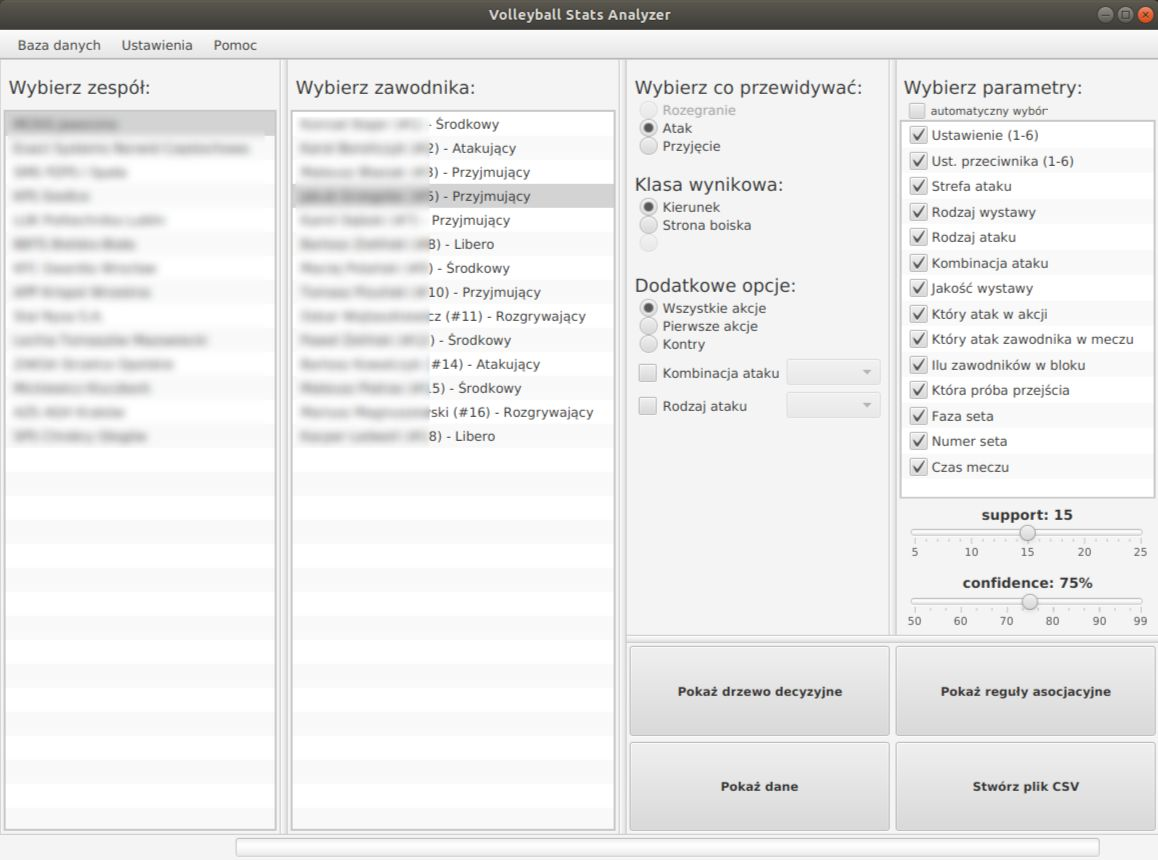
\includegraphics[width=\columnwidth]{interfejs}
\caption{Widok główny interfejsu aplikacji Volleyball Stats Analyzer.}
\label{fig:interfejs}
\end{figure}

Pod trzecią oraz czwartą kolumną znajdują się cztery przyciski wywołujące kolejno działanie metody drzew decyzyjnych, działanie metody reguł asocjacyjnych, wizualizacji danych oraz stworzenie pliku ,,csv'' z~danymi statystycznymi całej drużyny. Wyniki działania obu metod zostały przedstawione w~opisanych w~pracy badaniach, w~rozdziałach \ref{roz:wizDrzewa}, \ref{roz:wizReguly}. Za sprawą wizualizacji danych można zaobserwować natomiast jak wyglądają wzajemne zależności poszczególnych atrybutów. Na rysunku \ref{fig:dane} pokazano przykładową wizualizację danych dotyczących ataków zawodnika. Wybór atrybutów opisujących osie $x$ i~$y$, a~także atrybutu, którego wartości będą określać kolory danych jest dowolny. W~zamieszczonym przykładzie wykres prezentuje zależność kierunku od kombinacji ataku, a~poszczególne kolory punktów określają w~jakiej fazie seta wystąpiły poszczególne zagrania. Jako, że punkty te określone są przez wartości dyskretne i~na rzeczywistym wykresie pokrywałyby się, dzięki parametrowi nazwanemu ,,Jitter'' możliwe jest rozproszenie punktów i~zaobserwowanie w~ten sposób ich zagęszczenia dla poszczególnych wartości.

\begin{figure}
\centering
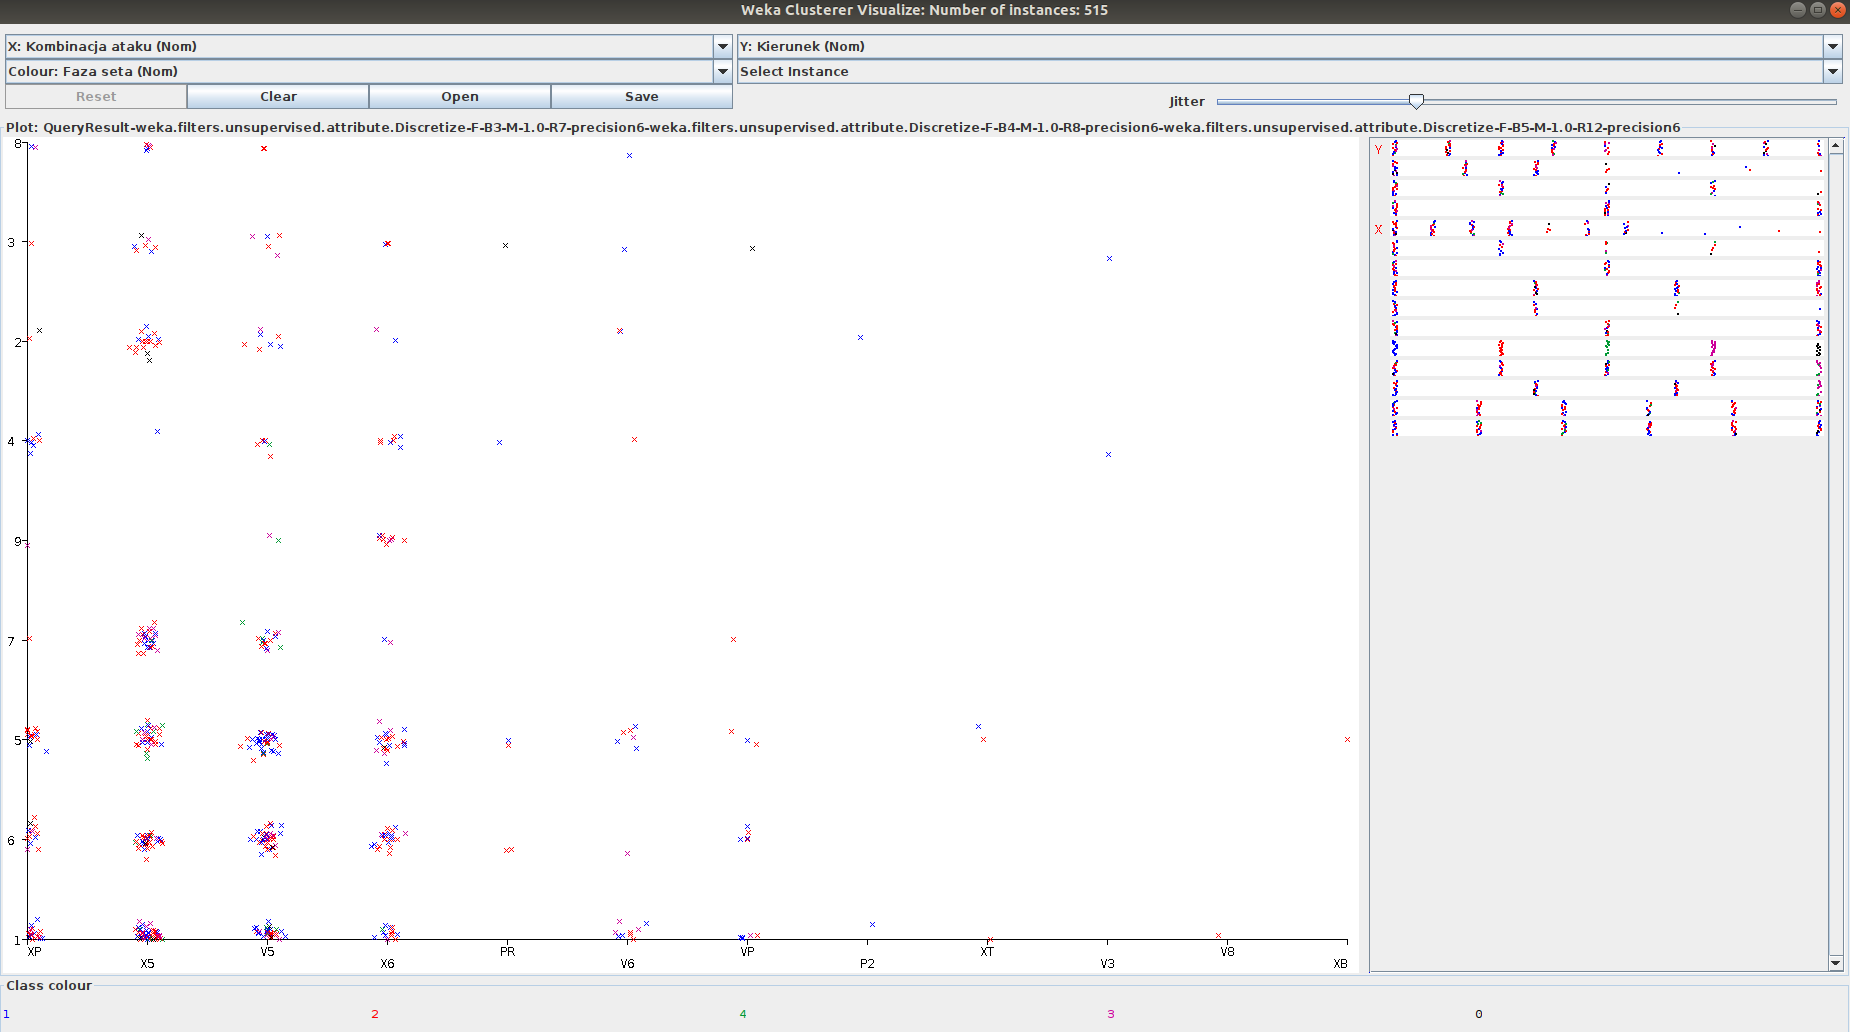
\includegraphics[width=\columnwidth]{dane}
\caption{Wizualizacja danych wybranych do analizy danego zawodnika.}
\label{fig:dane}
\end{figure}

W górnej zakładce programu nazwanej ,,Baza danych'' istnieje również możliwość wczytania oraz usunięcia meczów z~bazy danych, wybrania listy meczów na podstawie których mają zostać wykonane badania, a~także otwarcia innej bazy danych lub stworzenia całkiem nowej, na przykład dotyczącej innych rozgrywek lub innego sezonu. W~zakładce ,,Ustawienia'' istnieje natomiast możliwość zmiany języka. Dostępnymi językami są języki angielski oraz polski.


\chapter*{Spis skrótów i~symboli}

\begin{itemize}
\item[CAR] reguły asocjacyjne dla określonej klasy (ang. \ang{class association rules})
\item[CBA] klasyfikacja na podstawie asocjacji (ang. \ang{classification based on associations})
\item[CF] poziom ufności (ang. \ang{confidence factor})
\item[CRISP-DM] międzybranżowy standardowy proces eksploracji danych (ang. \ang{Cross-Industry Standard Process for Data Mining}) 
\item[$f_p$] liczba obserwacji błędnie przypisanych do analizowanej klasy (ang. \ang{false positive})
\item[$f_n$] liczba obserwacji analizowanej klasy przypisanych błędnie do innej klasy (ang. \ang{false negative})
\item[JDBC] łącze do baz danych w~języku Java (ang. \ang{Java Database Connectivity})
\item[pr] precyzja klasyfikacji (ang. \ang{precision})
\item[re] czułość klasyfikacji (ang. \ang{recall})
\item[SQL] strukturalny język zapytań (ang. \ang{Structured Query Language})
\item[$t_p$] liczba obserwacji dobrze przypisanych do analizowanej klasy (ang. \ang{true positive})
\end{itemize}


 

\chapter*{Zawartość dołączonej płyty}

Do pracy dołączona jest płyta CD z~następującą zawartością:
\begin{itemize}
\item praca w~formacie \texttt{pdf},
\item źródła programu,
\item zbiory danych użyte w~eksperymentach.
\end{itemize}

\listoffigures
\listoftables
	
\end{appendices}


\end{document}


%% Finis coronat opus.
